
%\documentclass[a4paper, titlepage]{report}
\documentclass[ALICE,manyauthors]{cernphprep}

%\usepackage{textcomp}
\usepackage[english]{babel}
\usepackage{fancyhdr}
\usepackage{amsmath}
\usepackage{graphicx}
\usepackage{verbatim}
\usepackage{lineno}
\usepackage{amsfonts}
\usepackage{makeidx}
\usepackage{color}
\pagestyle{headings}
\usepackage{epstopdf}
\usepackage{multirow}
\usepackage{hyperref}   % creates links to references, chapters etc and a separated table of contents in the .pdf file

%%%
%%%  Alias
%%%
\newcommand{\pp}{p-p}
\newcommand{\sqrts}{\sqrt{s}}
\newcommand{\sqrtsNN}{\sqrt{s_{\rm \scriptscriptstyle NN}}}
\newcommand{\lsim}{\,{\buildrel < \over {_\sim}}\,}
\newcommand{\gsim}{\,{\buildrel > \over {_\sim}}\,}
\newcommand{\av}[1]{\left\langle #1 \right\rangle}
\newcommand{\eV}{\mathrm{eV}}
\newcommand{\keV}{\mathrm{keV}}
\newcommand{\MeV}{\mathrm{MeV}}
\newcommand{\GeV}{\mathrm{GeV}}
\newcommand{\TeV}{\mathrm{TeV}}
\newcommand{\ev}{\mathrm{eV}}
\newcommand{\kev}{\mathrm{keV}}
\newcommand{\mev}{\mathrm{MeV}}
\newcommand{\gev}{\mathrm{GeV}}
\newcommand{\tev}{\mathrm{TeV}}
\newcommand{\fm}{\mathrm{fm}}
\newcommand{\mm}{\mathrm{mm}}
\newcommand{\cm}{\mathrm{cm}}
\newcommand{\m}{\mathrm{m}}
\newcommand{\mum}{\mathrm{\mu m}}
\newcommand{\s}{\mathrm{s}}
\renewcommand{\d}{\mathrm{d}}
\newcommand{\ns}{\mathrm{ns}}
\newcommand{\mrad}{\mathrm{mrad}}
\newcommand{\mb}{\mathrm{mb}}
\newcommand{\mub}{\mathrm{\mu b}}
\newcommand{\T}{\mathrm{T}}
\newcommand{\PbPb}{\mbox{Pb--Pb}}
\newcommand{\Npart}{N_{\rm part}}
\newcommand{\Ncoll}{N_{\rm coll}}
\newcommand{\Raa}{R_{\rm AA}}
\newcommand{\RAA}{R_{\rm AA}}
\newcommand{\TAA}{T_{\rm AA}}
\newcommand{\RCP}{R_{\rm CP}}
\newcommand{\pt}{p_{\rm T}}
\newcommand{\dNdy}{{\rm d}N_{ch}/{\rm d}y}
\newcommand{\momwin}{[$p$, $p$+$\Delta$ $p$]}
\newcommand{\DtoKpi}{{\rm D^0\to K^-\pi^+}}
\newcommand{\DtoKpipi}{{\rm D^+\to K^-\pi^+\pi^+}}
\newcommand{\DstartoDpi}{{\rm D^{*+}\to D^0\pi^+}}
\newcommand{\Dzero}{{\rm D^0}}
\newcommand{\Dstar}{{\rm D^{*+}}}
\newcommand{\Dplus}{{\rm D^+}}
\newcommand{\nbinv}{{\rm nb^{-1}}}
\newcommand{\decleng}{{\rm L}_{xyz}}
\newcommand{\dEdx}{{\rm d}E/{\rm d}x}
\newcommand{\mufac}{\mu_{\rm F}}
\newcommand{\muren}{\mu_{\rm R}}
%%%
%%% end Alias
%%%

\begin{document}
\begin{titlepage}


%\PHnumber{ALICE-2011-XYZ}                 % required, obtained from PH
\PHdate{\today}              % required

\title{D-hadron correlations  in p-Pb collisions at $\sqrt{s_\mathrm{NN}}$ = 5.02 TeV}

\Collaboration{F. Colamaria, S. Kumar, M. Mazzilli}%

\ShortAuthor{DRAFT \today, FOR INTERNAL USE ONLY}
\ShortTitle{D-hadron correlations}

\begin{abstract}
In this note, we present the analysis of azimuthal correlations of D mesons and primary charged $\pi$,K,p,e,$\mu$ performed in the ALICE central barrel in p-Pb collisions at $\rm{\sqrt{s_{NN}}}$ = 5.02 TeV, from 2016 data taking. The analysis is performed in an extended $\pt$ range and with additional observables with respect to p-Pb 2013 data analysis. After a description of the analysis strategy, corrections and systematic uncertainties, the results obtained for prompt $\Dzero$, $\Dstar$ and $\Dplus$mesons in different ranges of transverse momentum of the D meson and of the associated particles are presented. The results are then compared to Monte Carlo models and also with published 2013 p-Pb analysis results for the common $\pt$ ranges. %, namely $3<p_{T}^{D}<16$ GeV/$c$, $3<p_{T}^{D}<5$ GeV/$c$, $5<p_{T}^{D}<8$ GeV/$c$, $8<p_{T}^{D}<16$ GeV/$c$, and for the associated particles $p_T^{assoc}>0.3$ GeV/$c$ and $p_T^{assoc}>1$ GeV/$c$.

\end{abstract}


\end{titlepage}

\linenumbers
\tableofcontents

\newpage
\section{Introduction and Motivation}
%Two-particle azimuthal correlations in different kinematic ranges have played a crucial role in the understanding of jet production
%and modification in relativistic heavy-ion collisions, from RHIC to LHC energies.
%The extension of these studies to the heavy-flavour domain at the LHC will probe our understanding of QCD in the perturbative
%regime, accessible in a large kinematic range given the large mass of heavy quarks. Flavour conservation in QCD implies that charm quarks5are always produced as pairs of quarks and anti-quarks. The azimuthal correlations obtained using a meson carrying a heavy quark as trigger particle
%with the other charged particles in the same event give the possibility to study the underlying charm production mechanism in detail. In particular, prompt
%heavy quark pair production leads, at first order in leading-order pQCD, to back-to-back production. Heavy quarks produced by splitting of massless gluons are instead
% produced at small $\Delta\phi$. A third production process, the production
%by flavour excitation leads to a big separation in rapidity and most of the time one of the two quarks is produced in the forward region. \\

%Angular differential measurements of charm production are therefore interesting in their own right in pp collisions to study the structure
%and fragmentation of charm quarks, as well as their production mechanism. Correlations of  prompt charm meson pairs were first measured by Fermilab E791 Collaboration at Tevatron \cite{E791} also later by
%CDF II at Tevatron, showing a fair agreement with Pythia for the overall production, with some disagreement in the collinear and back-to-back production~\cite{CDF}. \\

%Heavy-flavour correlation studies in more complex collisional systems, like Pb-Pb aim to study the modification of the fragmentation of charmed jets due to in-medium (or cold nuclear matter, in case of p-Pb collisions) effects, in a similar fashion as it was done for di-hadron correlation studies in heavy-ion collisions (see for example~\cite{th1,th2}). Furthermore, the recent observation of long range correlations in p-Pb for light flavour hadrons and for heavy-flavour decay electrons %add reference
%points to possible collective effects or effects originating from gluon saturation in the initial state. More information could be extracted by the eventual observation of the same effect with D mesons.\\

%In the following, we describe the analysis strategy for p-Pb in all its steps, and we describe the list of corrections and the estimation of the systematic uncertainties
%done. After a section dedicated to detailed studies performed with Monte Carlo simulations to check the different analysis steps, we present the results of
%$\Delta\phi$ correlations obtained for prompt $D^0$, $D^{+}$ and $D^{*+}$ in different ranges of transverse momentum for the D-meson (trigger particle) and the associated particles.

The study of the azimuthal correlations of heavy-flavour particles and charged particles at the LHC energies provides a way to characterize charm production and fragmentation processes in pp collisions. The measurement also provide a way to probe our understanding of QCD in the perturbative regime, accessible in a large kinematic range given the large mass of heavy quarks. Flavour conservation in QCD implies that charm quarks are always produced as pairs of quarks and anti-quarks. The azimuthal correlations obtained using a meson carrying a heavy quark as trigger particle with the other charged particles in the same event give the possibility to study the underlying charm production mechanism in detail. In particular, prompt charm quark-antiquark pair production is back to back in azimuth at first order in leading-order perturbative-QCD (pQCD). If an hadron from the quark hadronization is taken as trigger particle, a near-side (at $\Delta\varphi = 0$) and an away-side (at $\Delta\varphi = \pi$) peak would appear in the azimuthal correlation distributions, coming from the fragmentation of the quark pair. Heavy quarks produced from the splitting of a massless gluon can be rather collimated and may generate sprays of hadrons at small $\Delta\varphi$. Finally, for hard-scattering topologies classified as ``flavour-excitation", a charm quark undergoes a hard interaction from an initial splitting ($g\to c\bar{c}$), leading to a big separation in rapidity of the hadrons originating from the antiquark (quark) with respect to the trigger D meson and contribute to a rather flat term to the $\Delta\phi$-correlation distribution.

Heavy-flavour correlation studies in more complex collision systems, like Pb-Pb, play a crucial role in studying the modification of the fragmentation of charmed jets due to in-medium (or cold nuclear matter, in case of p-Pb collisions) effects, in a similar way as it was done for di-hadron correlation studies in heavy-ion collisions (see for example). Furthermore, the recent observation of long range correlations in p-Pb for light flavour hadrons (\cite{ALICEv2ppb}, \cite{ALICEv2ppb2}) and for heavy-flavour decay electrons (ALICE preliminary results) points to possible collective effects or effects originating from gluon saturation in the initial state. More information could be extracted by the eventual observation of the same effect with D mesons.\\

In the following note, we first describe the analysis strategy for the p-Pb 2016 data sample in all its steps, followed by the list of analysis corrections and the estimation of systematic uncertainties. Finally the results of $\Delta\varphi$ correlations, and quantitative observable extracted to fits to those distributions, obtained for prompt $\rm{D^0}$, $\rm{D^{+}}$ and $\rm{D^{*+}}$ in different ranges of transverse momentum for the D-meson (trigger particle) and the associated particles are presented.


\newpage
\section{Data/Monte Carlo samples and event selection}
The data samples used for the analyses were the FAST and CENT$\_$woSDD samples from periods LHC16q and LHC16t (AOD samples). The reason for this choice is explained later on, in this section. It was verified, by looking at D-meson and track $\eta$ and $\varphi$ distributions, and at the mixed-event correlation distributions for each subsamples, that no visible differences arose for the four periods, hence it was possible to perform the analysis directly on the merged samples without any bias.

The Monte Carlo productions adopted for this study were:
 \begin{enumerate}
 \item LHC17d2a$\_$fast$\_$new, a HIJING production with enrichment, for each event, of c or b quarks and their decay chains, performed by PYTHIA6 with Perugia2011 tune, and with forced hadronic decays of the charmed hadrons. This production was used for D-meson efficiency evaluation, purity estimation and Monte Carlo closure test.
 \item LHC17a2b$\_$cent$\_$woSDD and LHC17a2b$\_$fast, minimum-bias samples produced with DPMJET generator, used for the evaluation of the tracking efficiencies.
\end{enumerate}

Table 1 shows the list of runs used for the analysis, for each of the data taking periods, and of the Monte Carlo productions used to evaluate the corrections:

% Systematic table
\begin{table}[h]
\begin{tabular}{ p{1.2cm} | p{4.2cm} |  p{7cm} |  p{1.2cm}}
{\normalsize \textbf {Type}} &       {\normalsize \textbf {Production}} &       {\normalsize \textbf {Run list}} & {\normalsize \textbf {nEvents}} \\
\\ \hline
Monte-Carlo & LHC17d2a$\_$fast$\_$new (c/b enriched), LHC17a2b$\_$fast (MB), LHC17a2b$\_$cent$\_$woSDD (MB) &267166, 267165, 267164, 267163, 265525, 265521, 265501, 265500, 265499, 265435, 265427, 265426, 265425, 265424, 265422, 265421, 265420, 265419, 265388, 265387, 265385, 265384, 265383, 265381, 265378, 265377, 265344, 265343, 265342, 265339, 265338, 265336, 265335, 265334, 265332, 265309 = \textbf{[36 runs]} & 50M\\
\\ \hline

\multirow{7}{*}{} Data&LHC16q, pass1$\_$CENT$\_$woSDD & 265525, 265521, 265501, 265500, 265499, 265435, 265427, 265426, 265425, 265424, 265422, 265421, 265420, 265419, 265388, 265387, 265385, 265384, 265383, 265381, 265378, 265377, 265344, 265343, 265342, 265339, 265338, 265336, 265335, 265334, 265332, 265309 = \textbf{[32 runs]}& 261M total\\
                  &LHC16q, pass1$\_$FAST &265525, 265521, 265501, 265500, 265499, 265435, 265427, 265426, 265425, 265424, 265422, 265421, 265420, 265419, 265388, 265387, 265385, 265384, 265383, 265381, 265378, 265377, 265344, 265343, 265342, 265339, 265338, 265336, 265335, 265334, 265332, 265309 = \textbf{[32 runs]} & 260M \\
% \\ \hline
 & LHC16t, pass1$\_$CENT$\_$woSDD & 267166, 267165, 267164, 267163 = \textbf{[4 runs]} & 40M \\
% \\ \hline
  & LHC16t, pass1$\_$FAST & 267166, 267165, 267164, 267163 = \textbf{[4 runs]} & 41M \\
 \hline \hline
\label{tab:Sample}
\end{tabular}
\\
\caption {Data Set and Run list}
\end{table}

The trigger mask request for the event selection is kINT7. Only events with a reconstructed primary vertex within 10 cm from the centre of the detector along the beam line are considered for both pp and p-Pb collisions. This choice maximises the detector coverage of the selected events, considering the longitudinal size of the interaction region, and
the detector pseudorapidity acceptances. For p-Pb collisions, the center-of-mass reference frame of the nucleon-nucleon collision is shifted in rapidity by $y_{\rm NN}$ = 0.465 in the proton direction with respect to the laboratory frame, due to the different per-nucleon energies of the proton and the lead beams.
Beam-gas events are removed by offline selections based on the timing information provided by the V0 and the Zero Degree Calorimeters, and the correlation between the number of hits and track segments in the SPD detector. This is automatically performed in the Physic Selection, a positive outcome of which is required during our event selection.
The minimum-bias trigger efficiency is 100\% for events with D mesons with $\pt > 1$ GeV/c. For the analyzed data samples, the probability of
pile-up from collisions in the same bunch crossing is below 2\% per triggered event (in most of the runs, well below 1\%). Events in which more than one primary interaction vertex is reconstructed with the SPD detector (with minimum of 5 contributors, and a $z$ distance greater than 0.8 cm) are
rejected, which effectively removes the impact of in-bunch pile-up events on the analysis. Out-of-bunch tracks are effectively rejected by the request of at least one point in the SPD, which has a very limited time acquisition window (300 ns). Indeed, though the default associated track selection requires a minimum of 2 points in the ITS, as it will be shown later on full compatibility of the corrected results with 2 and 3 minimum ITS clusters is obtained. For FAST and CENT$\_$woSDD samples, the latter case indirectly forces the presence of a point in the SPD.

Since data collected during p-Pb 2016 data taking are distinguished into two categories - one including SDD detector (CENT$\_$wSDD sample) and a second one without the SDD in the reconstruction, or in the acquisition (CENT$\_$woSDD and FAST samples, repsectively), a study of performance of the D-hadron correlation analysis with respect to the data samples employed has been carried out for $\Dstar$ and $\Dplus$ mesons (more sensitive to the presence of the SDD w.r.t. the $\Dzero$, due to their reconstruction from three decay tracks).

For this reason, the D-hadron correlation distribution has been compared on LHC16q$\_$pass1$\_$CENT$\_$wSDD and LHC16q$\_$pass1$\_$CENT$\_$woSDD and the relative statistical uncertainty has been estimated in order to understand if it was better to perform the analysis separately on the two data sample, applying in this case different corrections, or not.
In particular, it was crucial for the correlation analysis involving the $\Dstar$ meson because the track reconstruction efficiency of the soft pion is $\approx 10\%$ higher employing also the SDD information.
Figure \ref{wSSvswoSDD} shows the normalized azimuthal correlation distribution for low, mid and high $\pt$ for $\Dstar$ meson. Blue points are referred to the woSDD sample while red points represents wSDD data. Figure \ref{wSSvswoSDDuncertainty} shows the relative statistical uncentainty extracted from the azimuthal correlation distributions for the $\Dstar$ in different kinematic ranges.

\begin{figure}[!h]
\centering
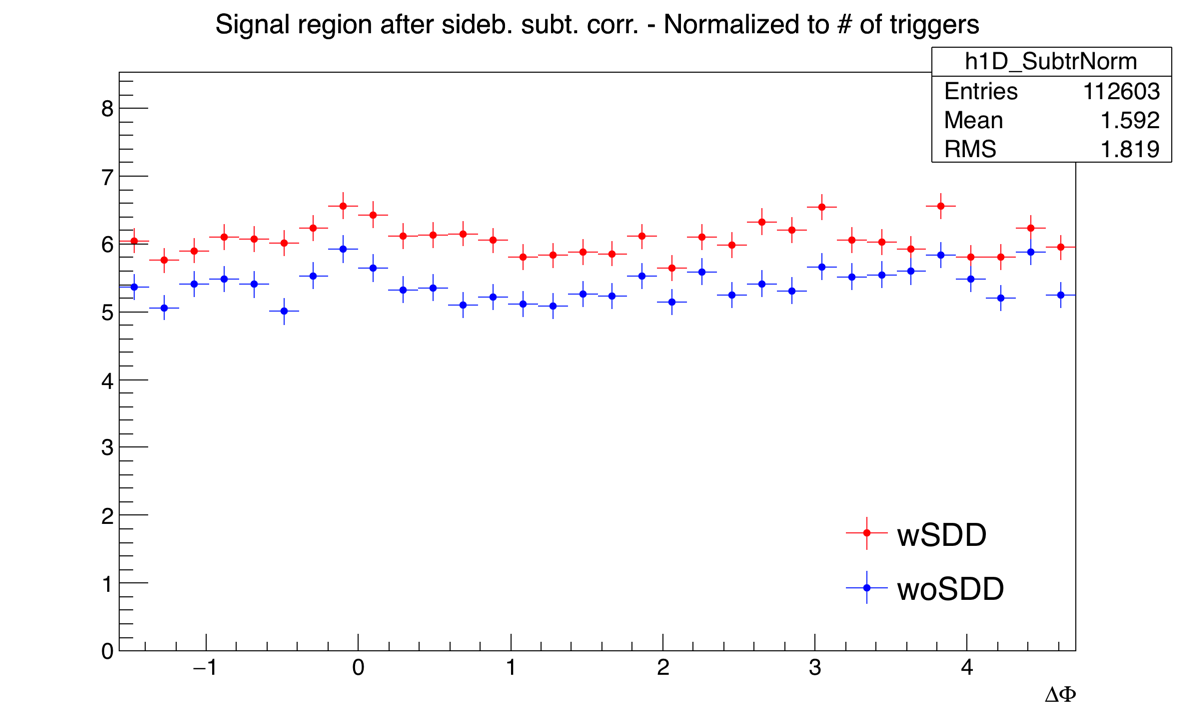
\includegraphics[width=0.8\linewidth, height=6cm]{figures/wSDD_vs_woSDD/AzimCorrDistr_Dstar_Canvas_PtIntBins2to3_PoolInt_thr0dot3to99dot0_Superimp.png}
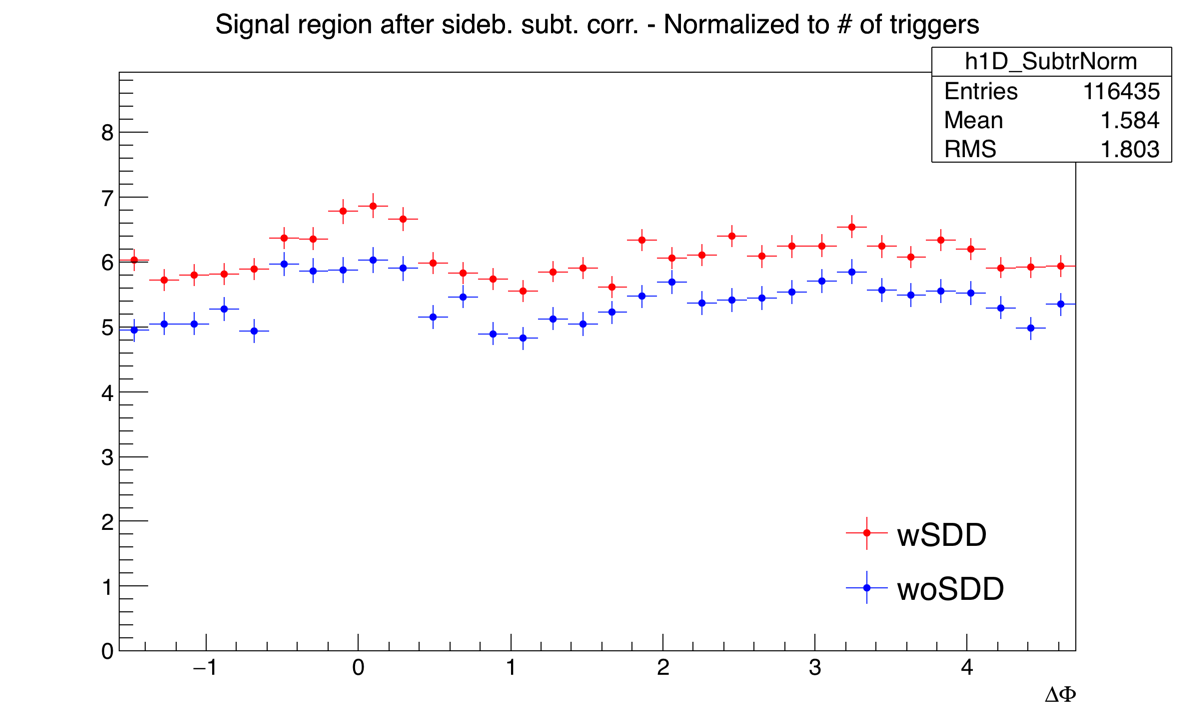
\includegraphics[width=0.8\linewidth, height=6cm]{figures/wSDD_vs_woSDD/AzimCorrDistr_Dstar_Canvas_PtIntBins4to6_PoolInt_thr0dot3to99dot0_Superimp.png}

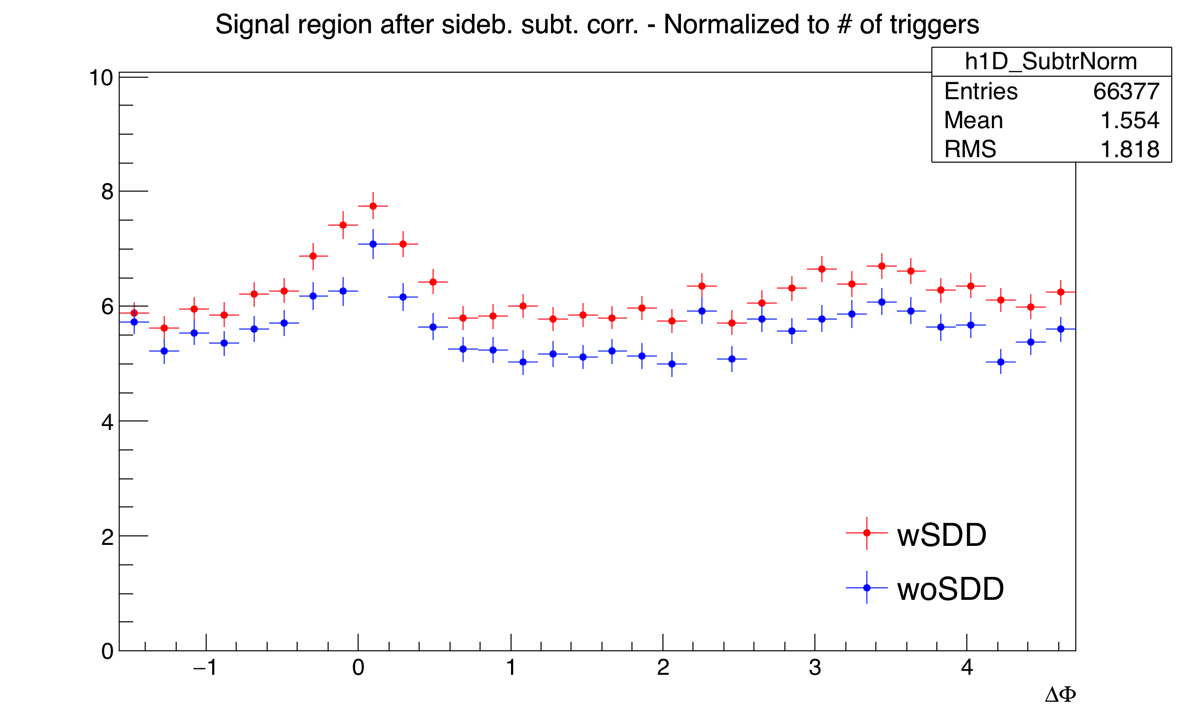
\includegraphics[width=0.8\linewidth, height=6cm]{figures/wSDD_vs_woSDD/AzimCorrDistr_Dstar_Canvas_PtIntBins7to9_PoolInt_thr0dot3to99dot0_Superimp.png}
\caption{Normalized azimuthal correlation distribution of $\Dstar$ for low $\pt$ ($3 < \pt(\Dstar) < 5$ GeV/c) on the top panel, mid $\pt$ ($5 < \pt(\Dstar) < 8$ GeV/c) on the middle panel and high $\pt$ ($8 < \pt(\Dstar) < 16$ GeV/c) on the bottom panel with a $\pt$ threshold for associated tracks of $\pt(assoc) > 0.3$ GeV/c. Blue points are referred to the woSDD sample while red points represent wSDD data.}
\label{wSSvswoSDD}
\end{figure}

\begin{figure}[!h]
\centering
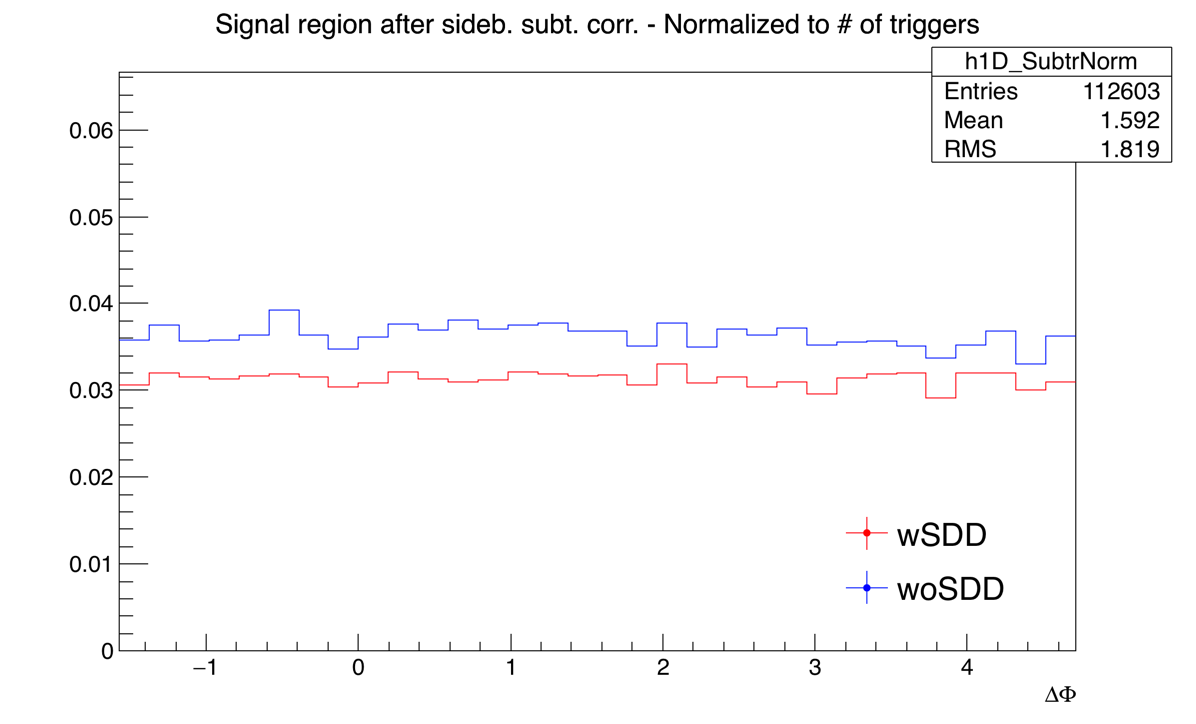
\includegraphics[width=0.8\linewidth, height=6cm]{figures/wSDD_vs_woSDD/Uncertanty_AzimCorrDistr_Dstar_Canvas_PtIntBins2to3_PoolInt_thr0dot3to99dot0.png}
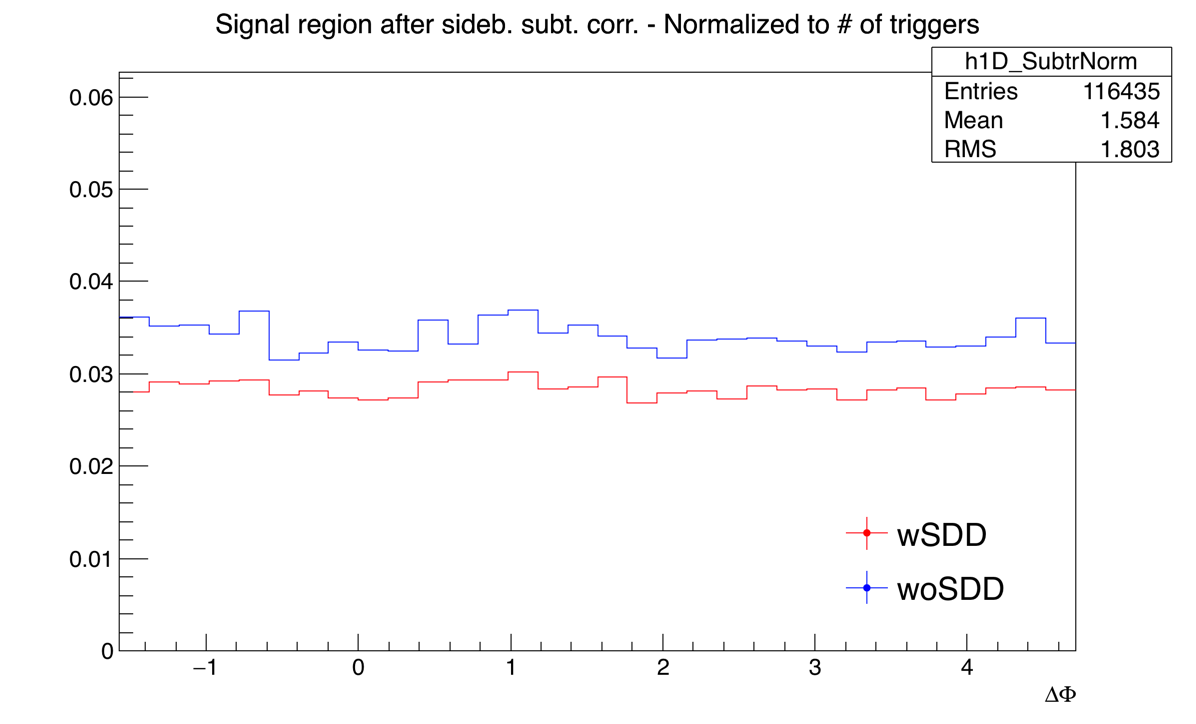
\includegraphics[width=0.8\linewidth, height=6cm]{figures/wSDD_vs_woSDD/Uncertanty_AzimCorrDistr_Dstar_Canvas_PtIntBins4to6_PoolInt_thr0dot3to99dot0.png}

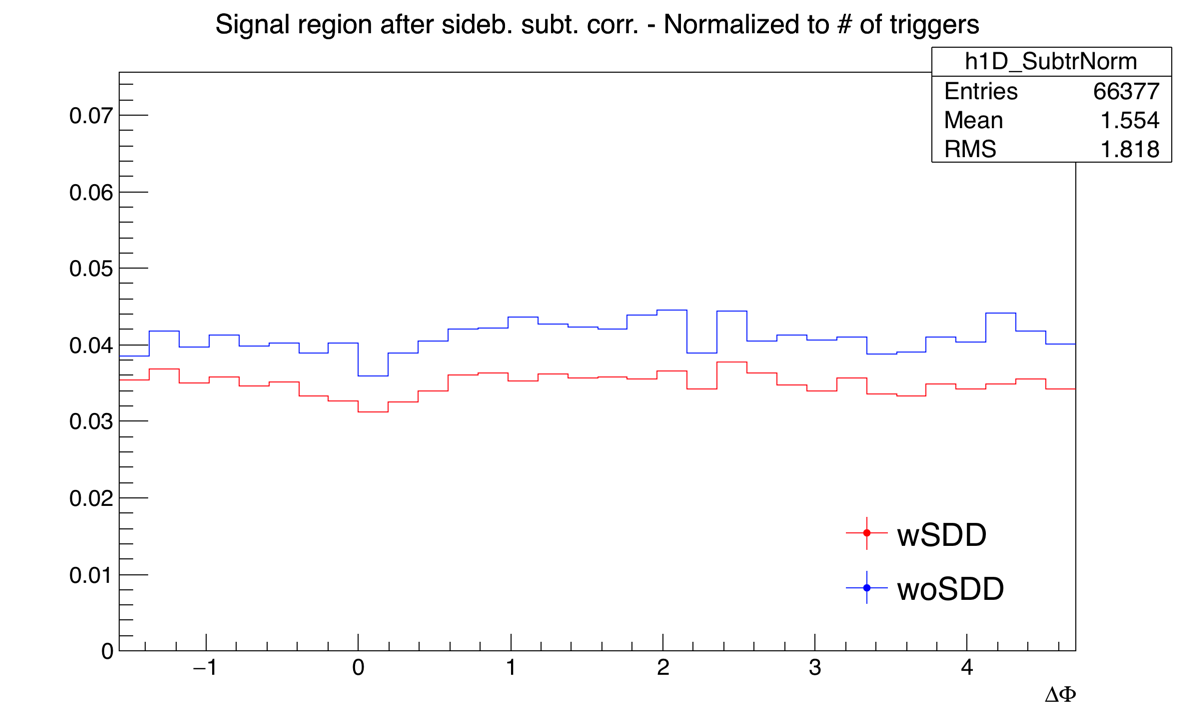
\includegraphics[width=0.8\linewidth, height=6cm]{figures/wSDD_vs_woSDD/Uncertanty_AzimCorrDistr_Dstar_Canvas_PtIntBins7to9_PoolInt_thr0dot3to99dot0.png}
\caption{Statistical uncertainty extracted from the azimuthal correlation distribution of $\Dstar$ with associated charged particles. Top panel: $3 < \pt(\Dstar) < 5$ GeV/c.
Mid panel: $5 < \pt(\Dstar) < 8$ GeV/c. Bottom panel: $8 < \pt(\Dstar) < 16$ GeV/c.
Blue line is referred to the woSDD sample while the red line represents wSDD data.}
\label{wSSvswoSDDuncertainty}
\end{figure}

It can be observed that the data sample that includes the SDD information is characterized by $\approx 10-15\%$ more statistics in each $\pt$ ranges analyzed. This difference is related to the larger efficiency in track reconstruction with the wSDD sample - a larger number of tracks survives to the selection request of 3 points in the ITS, which is part of the selection requests applied on the previous D-h analysis.

As a result, the wSDD sample is also affected by a slightly lower relative statistical uncertainty (about 12-15\%) due to several reasons: the larger tracking efficiency, the major number of signal entries in the invariant mass distributions and a slight increase of S/B, which reflects in a slight decrease of uncertainty from the sideband subtraction.
It has also to be considered that, on the full sample including also the FAST cluster, the increase in performance would be further reduced.
The overall statistical uncertainty difference resulting from the comparison is not enough to justify the implementation of two different analysis and two subsequent different corrections either for $\Dstar$ and $\Dplus$.

Anyway, to cope with the lower tracking efficiency w.r.t. 2013 data sample, after this study it was decided to reduce the ITS request for the associated tracks from 3 (used on 2013 data) to 2 ITS clusters as default selection criterion.




\newpage
\section{Analysis strategy}
The analysis follows the same strategy one used in 2013 p-Pb data sample (see published paper \cite{ALICEDhcorr} and analysis notes \cite{Notepp}, \cite{NotepPb}). Correlation pairs are formed by
trigger particles (D mesons) reconstructed and selected in the following $\pt^{\rm trig}$ ranges: $3<\pt^{\rm trig}<5$ $\gev/c$, $5<\pt^{\rm trig}<8$ $\gev/c$, $8<\pt^{\rm trig}<16$ $\gev/c$, $16<\pt^{\rm trig}<24$ $\gev/c$, and associated particles (charged tracks) for the following $\pt^{\rm assoc}$ regions: $\pt^{\rm assoc}>0.3$ $\gev/c$, $0.3<\pt^{\rm assoc}<1$ $\gev/c$, $1<\pt^{\rm assoc}<2$ $\gev/c$, $2<\pt^{\rm assoc}<3$ $\gev/c$, $\pt^{\rm assoc}>3$ $\gev/c$ (with the addition of $\pt^{\rm assoc}>1$ $\gev/c$ for comparison with p-Pb 2013 results). In this analysis, the particle identification defines the trigger particle rather than a momentum cut and therefore the momentum range of the associated particles is not constrained by that of the trigger particle. Our definition of associated particle includes primary particles of the following species: pion, kaon, proton, electron, muon. The primary particle definition comprises particle coming from the primary vertex of interaction, including those coming from strong and electromagnetic decay of unstable particles, and particles deriving from the decay of hadrons with charm or beauty.
We therefore include any charged $\pi$,K,p,e,$\mu$ except those coming from weak decays of strange particles and particles produced in the interaction with the detector material. This definition corresponds to that used in the method AliAODMCParticle::IsPyhysicalPrimary().
All associated particles surviving the selection cuts and not matching the adopted criterion are considered as a contamination whose contribution has to be corrected for. \\

The analysis is performed through the following steps:

\begin{enumerate}
\item
\underline {\bf D meson selection and signal extraction.}  For each single event, ``trigger" particles
are defined as the selected  D meson candidates ($\Dzero$, $\Dplus$ and $\Dstar$)
within a given $\pt^{\rm trig}$ range. The detection strategy for D mesons at central rapidity is
the same performed for the analyses of the D-meson production at central rapidity~\cite{ALICEDmespp7Tev}, and also applied for the D-h analysis on 2010 pp and 2013 p-Pb samples~\cite{ALICEDhcorr}. It is based on the reconstruction of decay
vertices displayed from the primary vertex by a few hundred $\mu$m and on the identification of the decay-particle species.
The identification of the charged kaon and pion in the TPC and TOF
detectors is also used, to further reduce the background at low $\pt$.  An
invariant-mass analysis is then used to extract the raw signal yield, using
the same fit functions described in~\cite{ALICEDhcorr}.
The D mesons are selected in the rapidity range varying from $|y|<0.5$ at low $\pt$ to $|y|<0.8$ for $\pt>5~\gev/c$. %The final results are corrected to have D mesons within $|y|<0.5$.

\item
\underline{\bf Correlation of D candidates with associated tracks.}
Particle pairs are formed by correlating each trigger particle with
the charged primary particles passing the track selection (excluding those coming from the decay of the D-meson candidate) in a specified $p^{assoc}_{T}$
interval (which can overlap with the $\pt^{\rm trig}$ range) and in the pseudo-rapidity range $|\eta|<0.8$. For the $\Dzero$ meson, also the low-momentum pion tracks from feed-down of $\Dstar$ mesons are removed via 3$\sigma$ invariant mass cut on the $M(K\pi\pi)-M(K\pi)$ difference. This because these soft pion are not related to the charm quark fragmentation chain.
For D meson candidates in the invariant mass signal region, defined by a $\pm$ 2$\sigma$ interval around the D meson mass peak, the azimuthal angle difference $\varphi^{\rm assoc}-\varphi^{\rm trigg}\equiv\Delta\varphi$
and the pseudorapidity difference $\eta^{\rm assoc}-\eta^{\rm trig}\equiv\Delta \eta$ are evaluated and stored to build two-dimensional correlation distribution. % in a multi-dimensional histogram.

\item
\underline{\bf Correction for limited acceptance and detector inhomogeneities with Event Mixing}
The angular correlation distribution may be affected, even for uncorrelated pair of particles, by structures not due to physical effects, but originating from the limited detector acceptance, as well as from angular inhomogeneities in the trigger and track reconstruction efficiencies as a function of $\Delta\varphi$ and $\Delta\eta$.
Effects of this kind are removed using the Event Mixing technique.
In this technique, the analysis is executed on the same data sample of the standard one (called ``same event" analysis, SE), but the trigger particles found in each event are correlated to charged particles reconstructed in different events (``Mixed Events'' analysis, ME) with similar characteristic, in particular concerning the event multiplicity and z position of the primary vertex (see Section \ref{MEsection}). \\

The differential yield of associated particles per trigger particle is obtained by
\begin{linenomath}
  \begin{equation}
    \label{2pcorr_incl}
    \frac{1}{N_\text{trig}}\frac{\d^{2}N^\text{pair}}{\d\Delta\eta\, \d\Delta\varphi}
= B_{ME}(0,0)\times\frac{S(\Delta\eta,\Delta\varphi)}{B_{ME}(\Delta\eta,\Delta\varphi)},
\end{equation}
\end{linenomath}
where $N^\text{pair}$ is the total number of correlated D-hadron
pairs. The functions $S(\Delta\eta,\Delta\varphi)$ and
$B_{ME}(\Delta\eta,\Delta\varphi)$ are the signal and the mixed event
background distributions, respectively. The later is normalized to its value in
$(\Delta\eta,\Delta\varphi)=(0,0)$, i.e. ($B(0,0)$).
Further details on the mixed-event correction are provided in the next section.

\item
\underline{\bf Subtraction of background correlation from signal distribution.}
The invariant mass signal region also includes background D-meson candidates. Their contribution to the
raw correlation distribution is subtracted as follows. For each $\pt$ bin, the mean and the sigma of the
invariant mass spectrum are extracted. For $\Dzero$ and $\Dplus$, a ``background'' region is defined in the sidebands of the mass
distribution as the interval $4 ~ \gev/c^2<|m-m^{\rm pdg}|<8 ~ \gev/c^2$ (for the $\Dstar$ meson, only the right sideband is used). The angular correlation distribution
for background candidates in this region is extracted and normalized with respect to the background in the signal region
estimated from the mass fit. This normalized background correlation distribution is then subtracted from the
raw signal one to obtain the signal correlation distribution. The normalization factor is the ratio of the number of background candidates under the signal peak (obtained by integrating the background of the fit function within the signal region) over the number of background candidates in the sidebands (obtained via bin-counting in the sideband region).
An example of the signal region, sideband and sideband-subtracted 1D correlation distributions (along $\Delta\varphi$ is shown in figure \ref{signReg}, together with the comparison of the three distributions after the normalization to the number of triggers.

\begin{figure}[h]
\centering
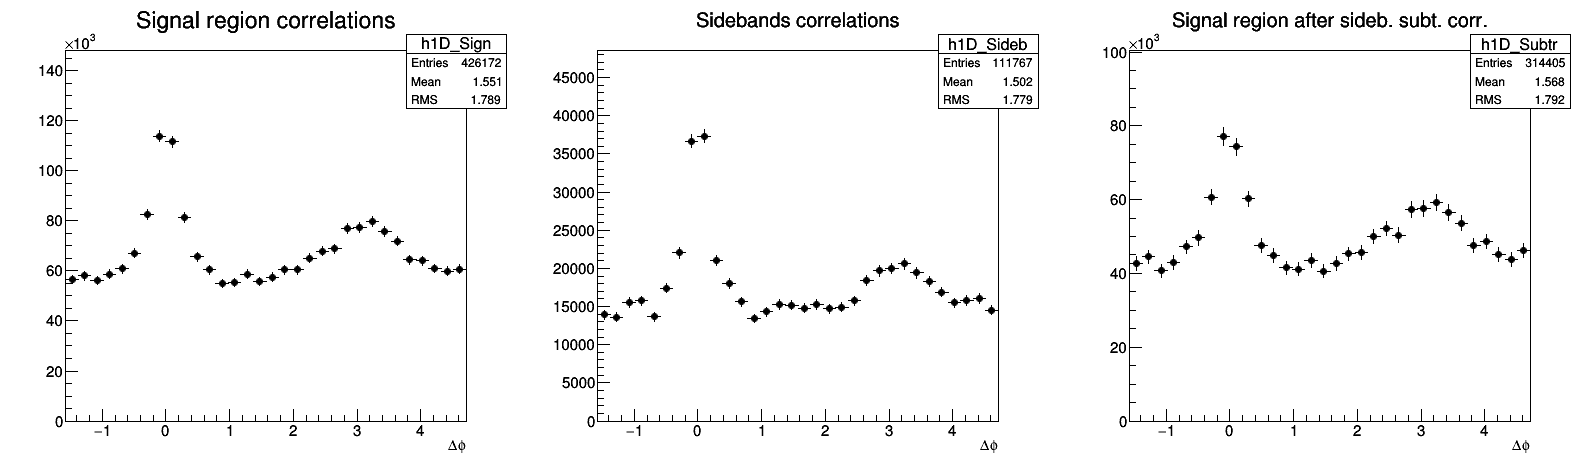
\includegraphics[width=1\linewidth]{{figures/Dzero/h1D_Dzero_Canvas_PtIntBins9to11_PoolInt_thr1dot0to99dot0.png}}
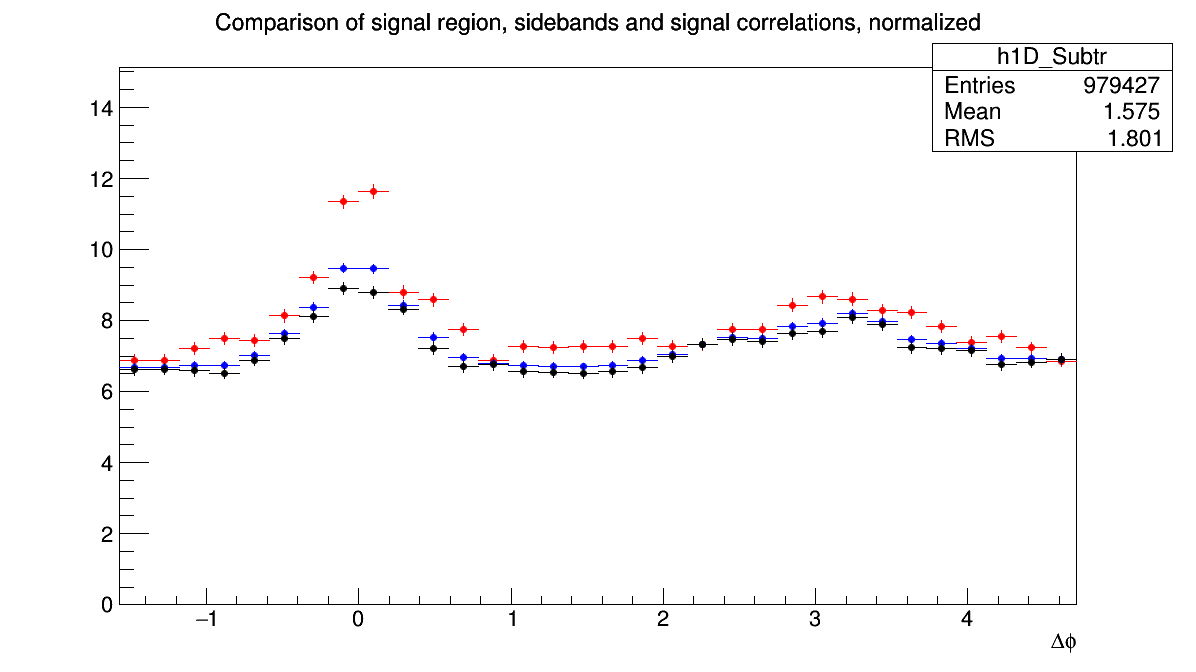
\includegraphics[width=0.8\linewidth]{{figures/Dzero/h1D_Dzero_Canvas_Normalized_PtIntBins9to11_PoolInt_thr0dot3to99dot0.png}}
\caption{Top: Example of $\Dzero$-h signal region (left), sideband (middle), and signal minus sideband (right) correlation distributions. Bottom: signal region per-trigger normalized correlation distribution (blue), sideband region per-trigger normalized correlation distribution (red),
background-subtracted per-trigger normalized correlation distribution (black).}
\label{signReg}
\end{figure}

\item
\underline{\bf Correction for D meson efficiency and associated track efficiency.}
After filling the signal and background correlation distributions, it is necessary to take into account also for the correlations with tracks, those are not reconstructed, or not passing the quality selection due to poor reconstruction. In the same way, the loss of D-mesons which are not reconstructed, or do not pass the selection, impacts the correlation distribution shape. Hence, each pair is weighted by the
inverse of the product of the associated track and D meson reconstruction efficiency, $\epsilon_{trk}$ and $\epsilon_{trig}$. Further details are provided later on in this section.

\item
\underline{\bf Projection in $\Delta\varphi$.}
The limited statistics available does not allow to study the two dimensional
$(\Delta\eta,\Delta\varphi)$ distribution, which is therefore projected to the $\Delta\varphi$ axis by integrating on $|\Delta\eta| <$ 1. Despite, in principle, our maximum $\Delta\eta$ acceptance is of $|\Delta\eta| <$ 1.6, removing the large $|\Delta\eta|$ regions allow us to reject angular regions with very low statistics, where fluctuations would be amplified by a large mixed-event correction, and avoid the so-called wings effect.

As the difference in the azimuthal angle is periodic ($\Delta \varphi = 0 = 2\pi$), the $\Delta\varphi$-range is limited to the essential range of 2$\pi$. The $\Delta \varphi$-limits are chosen to be [$-\pi$/2, 3$\pi$/2] in order to provide a good visibility of the correlation pattern, which peaks around 0 and $\pi$.

\item
\underline{\bf Correction for the contamination of secondary particles}
The DCA to primary vertex cut, applied during the associated track selection, has the role of removing the secondary particles from the associated track sample.
Secondary particles are indeed produced either from long-lived strange hadrons or from interaction of particles with the detector material. A residual contamination from secondary tracks is hence expected in the correlation distributions. This contamination is estimated from Monte Carlo simulation
based on Pythia as described more in detail in the next section. The background-subtracted
event-mixing corrected correlations are multiplied by a purity factor to encounter this contribution.

\item
\underline{\bf Correction for bias on B to D decay topologies}
The presence of the topological cuts for the D-meson selection indirecly induce a bias on the topology of the B to D recay topologies, favouring cases with a small opening angle between the D-meson and the other tracks from the B decay. This affects the feed-down component of the data correlation distributions. This effect is corrected for with a procedure described in the subsection \ref{MCclosure}. Note that this correction is a novelty with respect to the previous analyses, where only a quite conservative systematic uncertainty was applied to take into account this effect.

\item
\underline{\bf Correction for feed-down of D meson from b-hadron decay}
The selection strategy employed for the D meson candidates selection %to increase the signal over the combinatorial background
enhances the fraction of reconstructed D mesons coming from the decay of a b-hadron. Typical values, with the cuts used for the D-meson selection, are of the order of 10\% or less. The correlation distribution of these secondary D mesons will be sensitive to the properties of beauty jets and beauty hadron decay, which in general differ from those relative to charm jets and hadrons. The procedure used to subtract this contribution is described in the next paragraphs of this section.

\item
\underline{\bf Study of correlation properties.}
The properties of the azimuthal correlation distribution are quantified by
fitting the distribution with a function composed of two Gaussian functions, modelling the near and the away side peaks, and
a constant term describing the baseline. The mean of the Gaussian are fixed at
$\Delta\varphi = 0$ and $\Delta\varphi = \pi$. To accomplish the $2\pi$ periodicity
of the $\Delta\varphi$ variable, the Gaussian functions
are ``duplicated'' with mean at $\Delta\varphi = 2\pi$ and $\Delta\varphi = -\pi$.
The fitting procedure is described in details in Section \ref{results}.


%The integral of the near side peak and the away side peak
%is dominated by the central parts of the peaks at
%$\Delta \varphi = 0$ and $\Delta \varphi = \pi$, respectively. Thus, minor
%shape deviations at the side of the peak regions are  acceptable. In
%the following, the fit function is introduced step by step.
%The $\Delta \varphi$ distribution can roughly be approximated by a
%constant and two Gaussian functions with the periodicity condition.
%As the $\Delta \varphi$-distribution is a periodically continuing
%distribution with $\Delta\varphi = 0 = 2\pi$, the fit function has to
%be periodically continuing as well.

\end{enumerate}

\subsection{Mass plots and cut optimization}
The invariant mass distributions of $\Dzero$, $\Dstar$ and $\Dplus$ in the various pt ranges are shown in Figure~\ref{fig:InvMassD0},~\ref{fig:InvMassDs} and~\ref{fig:InvMassDp} respectively. Note that the distributions are weighted by the D-meson selection and reconstruction efficiency, to allow a correct normalization of the correlation distributions, which have also these weights.

\begin{figure}[!htp]
\centering

{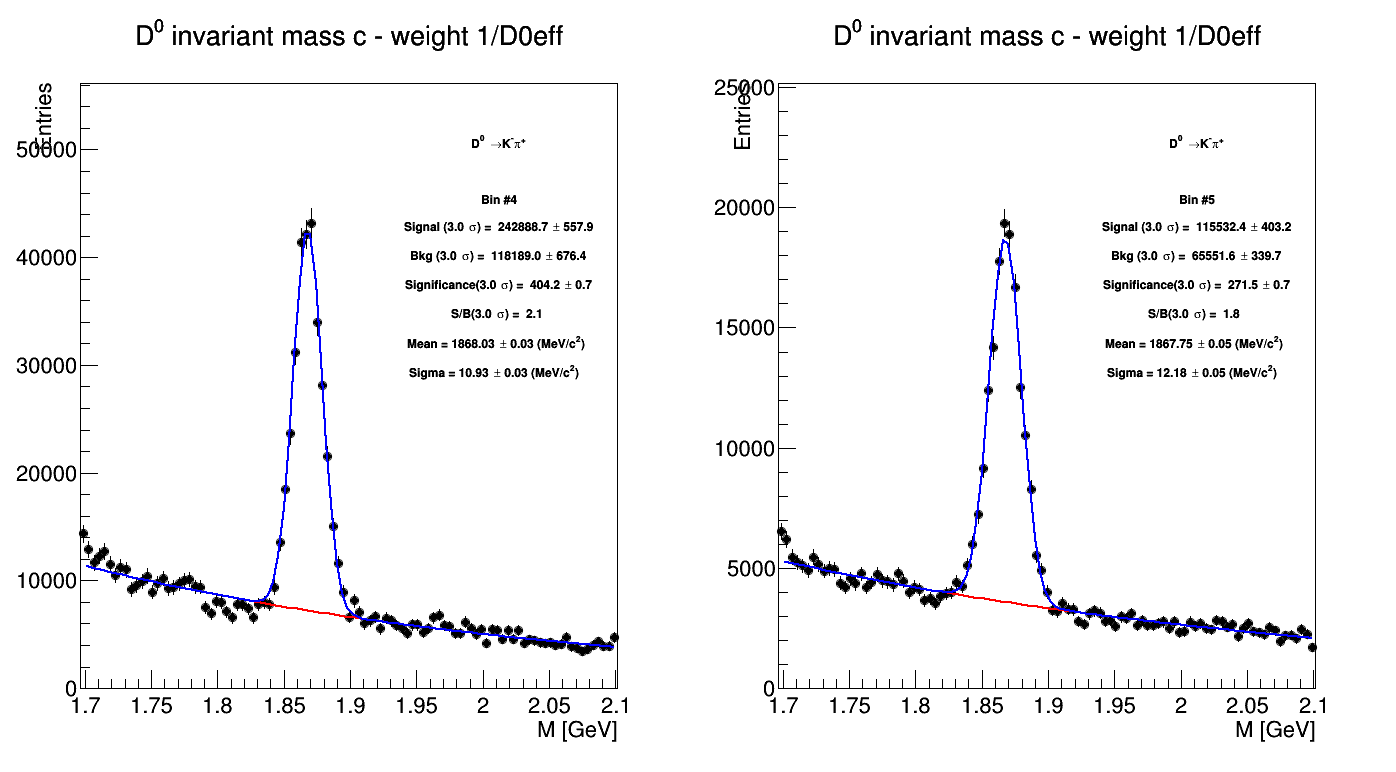
\includegraphics[width=1\linewidth, height=5.6cm]{figures/Dzero/InvMassDistributions_Dzero_Bins4to5.png}}
{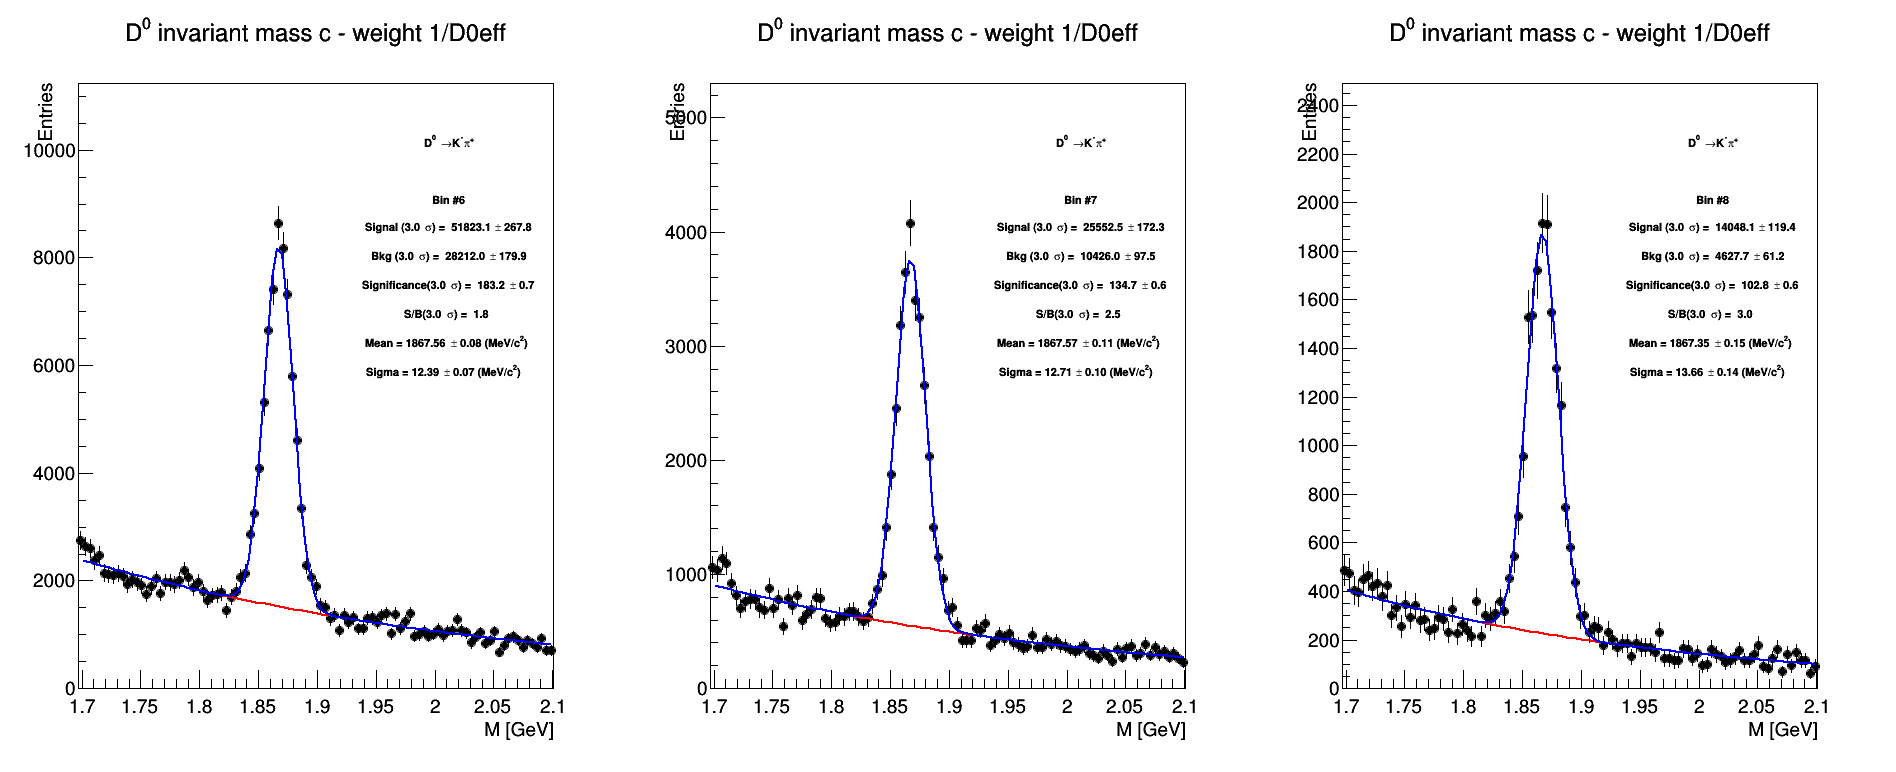
\includegraphics[width=1\linewidth, height=5.6cm]{figures/Dzero/InvMassDistributions_Dzero_Bins6to8.png}}
{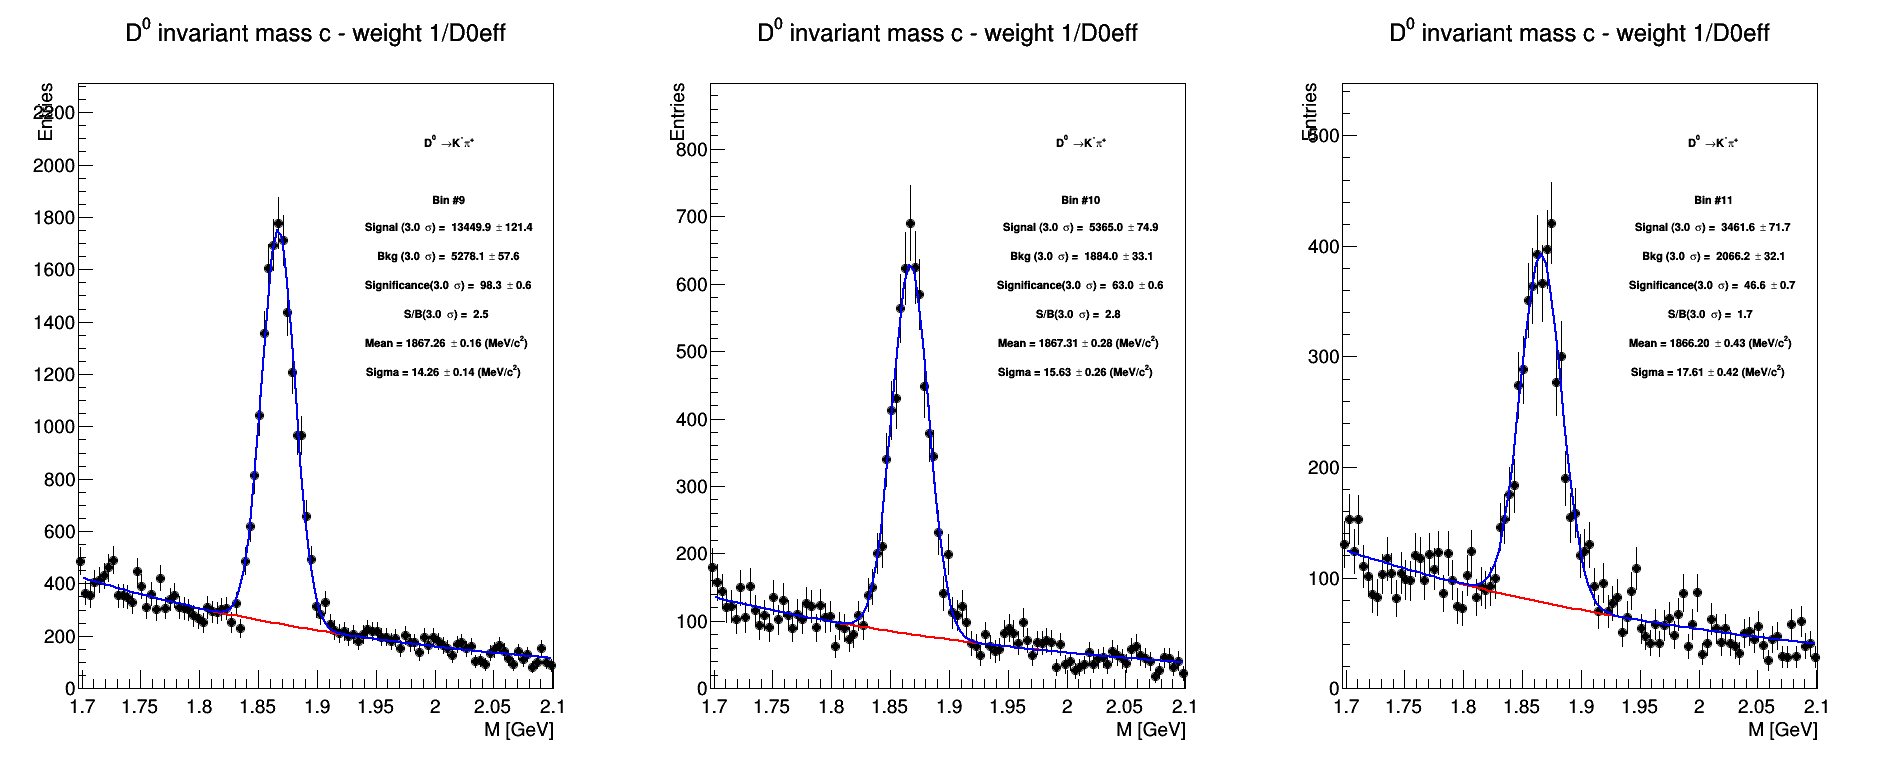
\includegraphics[width=1\linewidth, height=5.6cm]{figures/Dzero/InvMassDistributions_Dzero_Bins9to11.png}}
{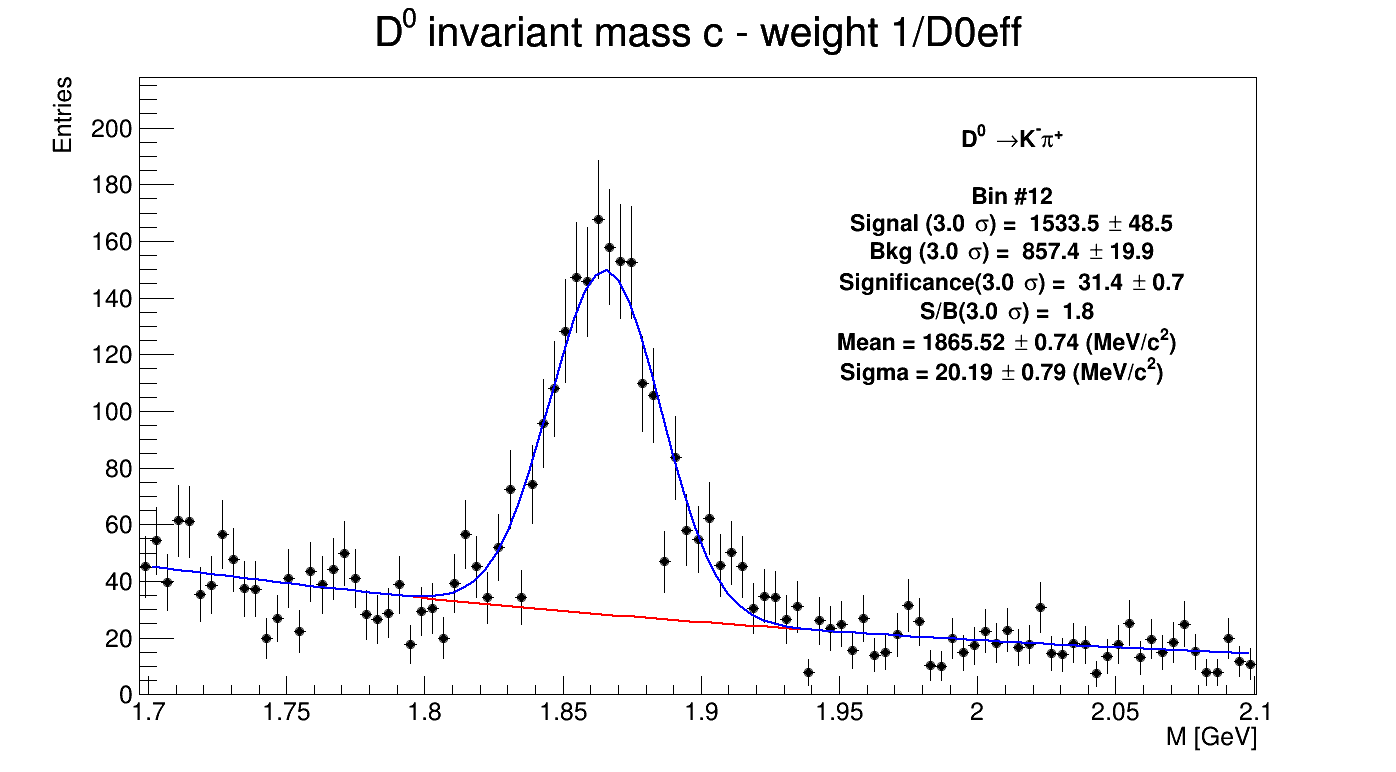
\includegraphics[width=0.6\linewidth, height=5.6cm]{figures/Dzero/InvMassDistributions_Dzero_Bins12to12.png}}

%[width=.32\linewidth]
\caption{Invariant mass distributions of $D^0$ corrected with efficiency in different $\text{p}_T$ regions. Top: $3< p_{T}^{\text{D}}< 4$ $\gev/c$ (left), $4< p_{T}^{\text{D}}< 5$ $\gev/c$ right), Mid 1: $5< p_{T}^{\text{D}}< 6$ $\gev/c$ (left), $6 < p_{T}^{\text{D}} < 7$ $\gev/c$ (middle), $7< p_{T}^{\text{D}}< 8$ $\gev/c$ (right); Mid2: $8< p_{T}^{\text{D}}< 10$ $\gev/c$, $10< p_{T}^{\text{D}}< 12$ $\gev/c$  (middle), $12 < p_{T}^{\text{D}}< 16$ $\gev/c$  (right) and Bottom: $16<p_{T}^{\text{D}}< 24$ $\gev/c$.}
\label{fig:InvMassD0}
\end{figure}

\begin{figure}[!htp]
\centering
{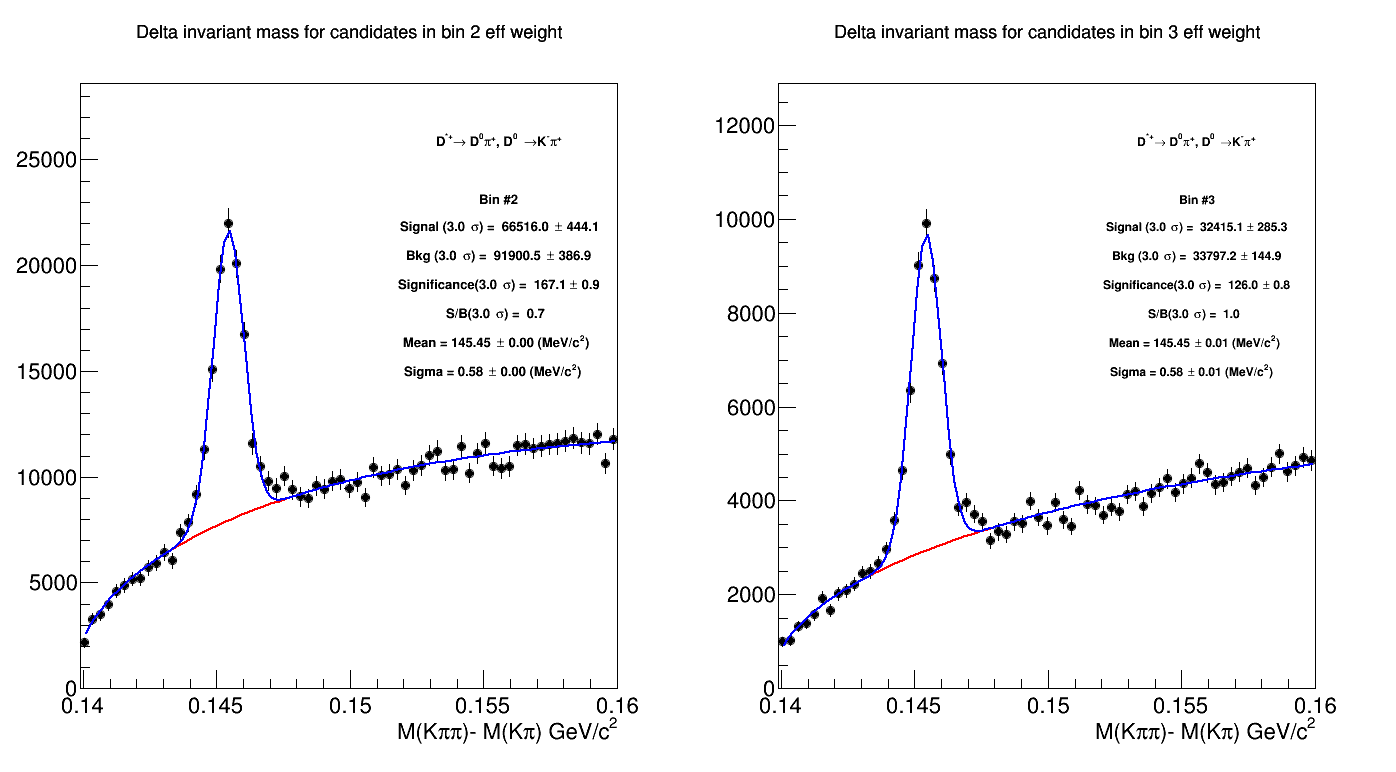
\includegraphics[width=1\linewidth, height=5.6cm]{figures/Dstar_wEFF/InvMassDistributions_Dstar_Bins2to3.png}}
{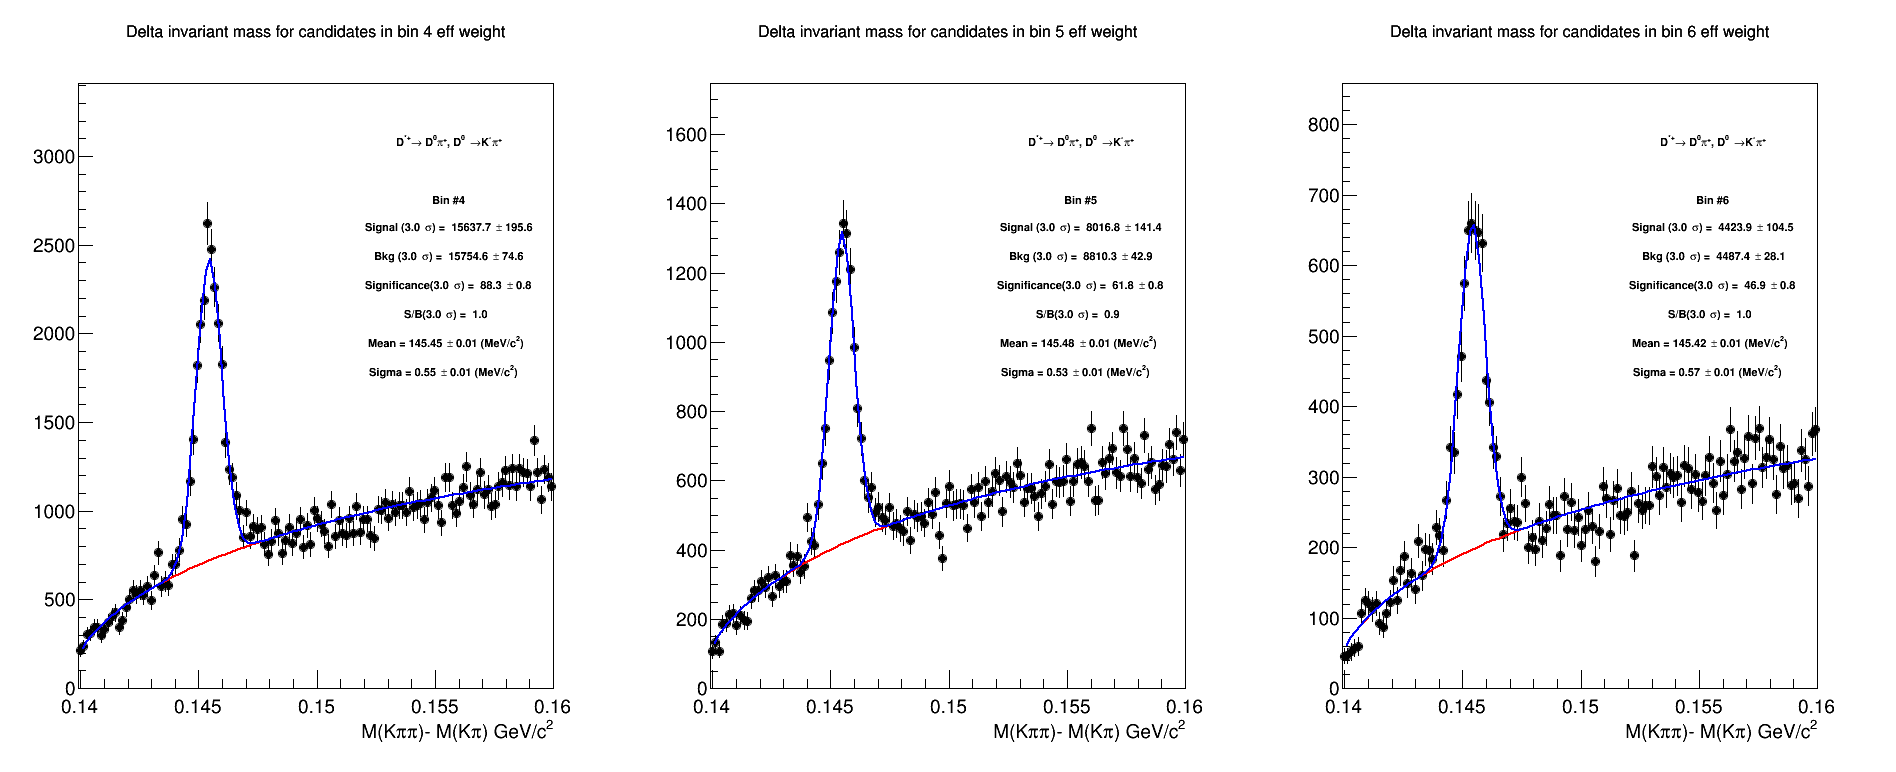
\includegraphics[width=1\linewidth, height=5.6cm]{figures/Dstar_wEFF/InvMassDistributions_Dstar_Bins4to6.png}}
{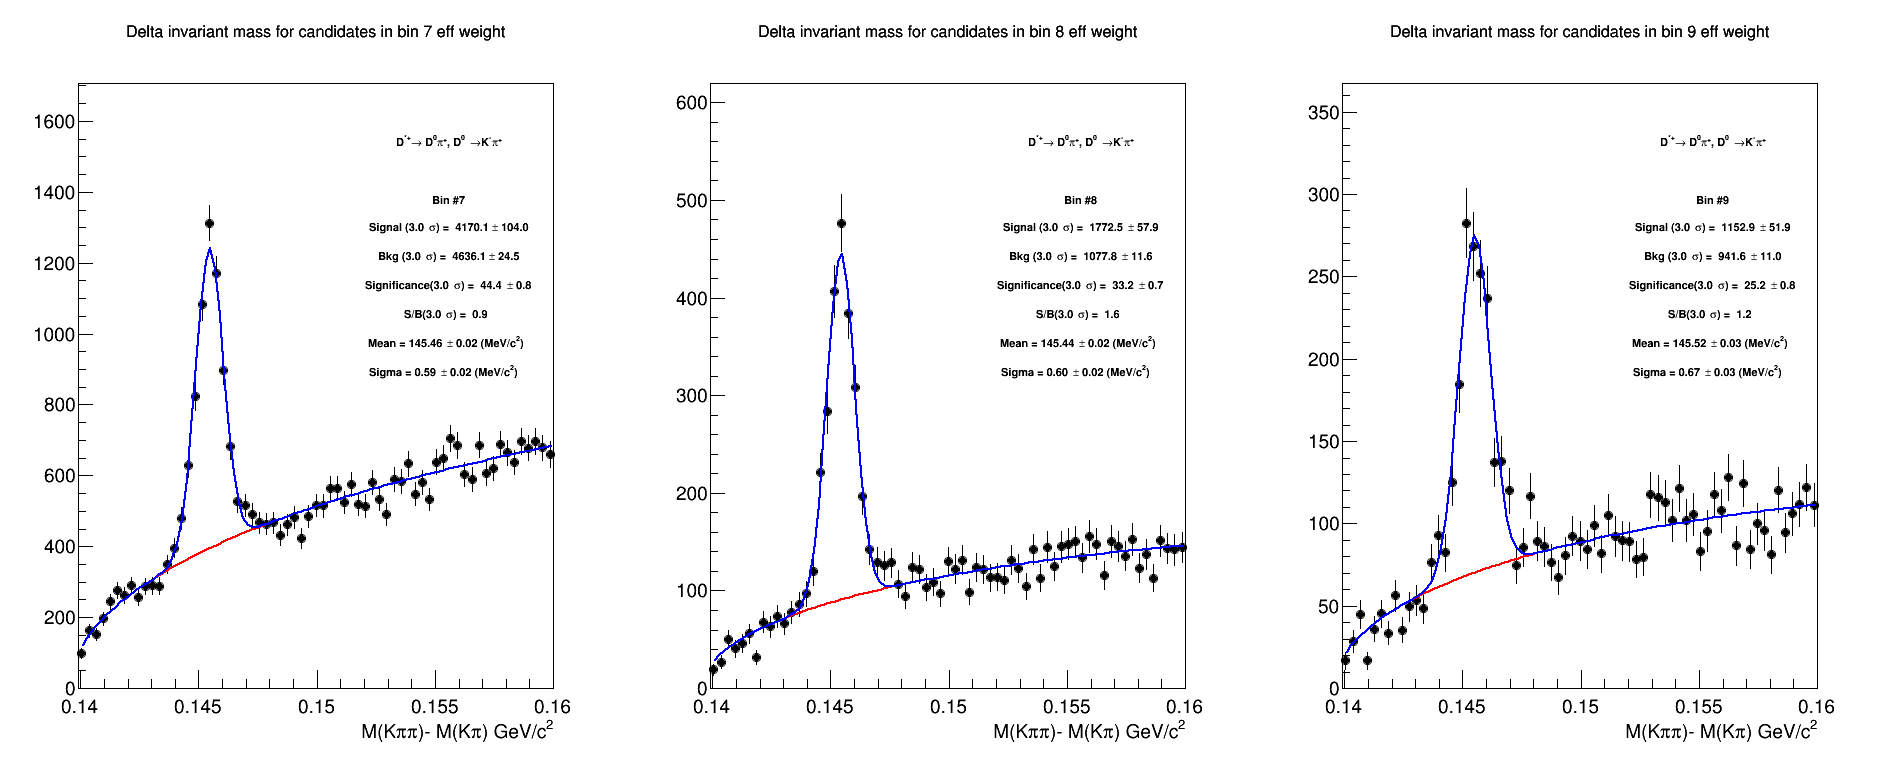
\includegraphics[width=1\linewidth, height=5.6cm]{figures/Dstar_wEFF/InvMassDistributions_Dstar_Bins7to9.png}}
{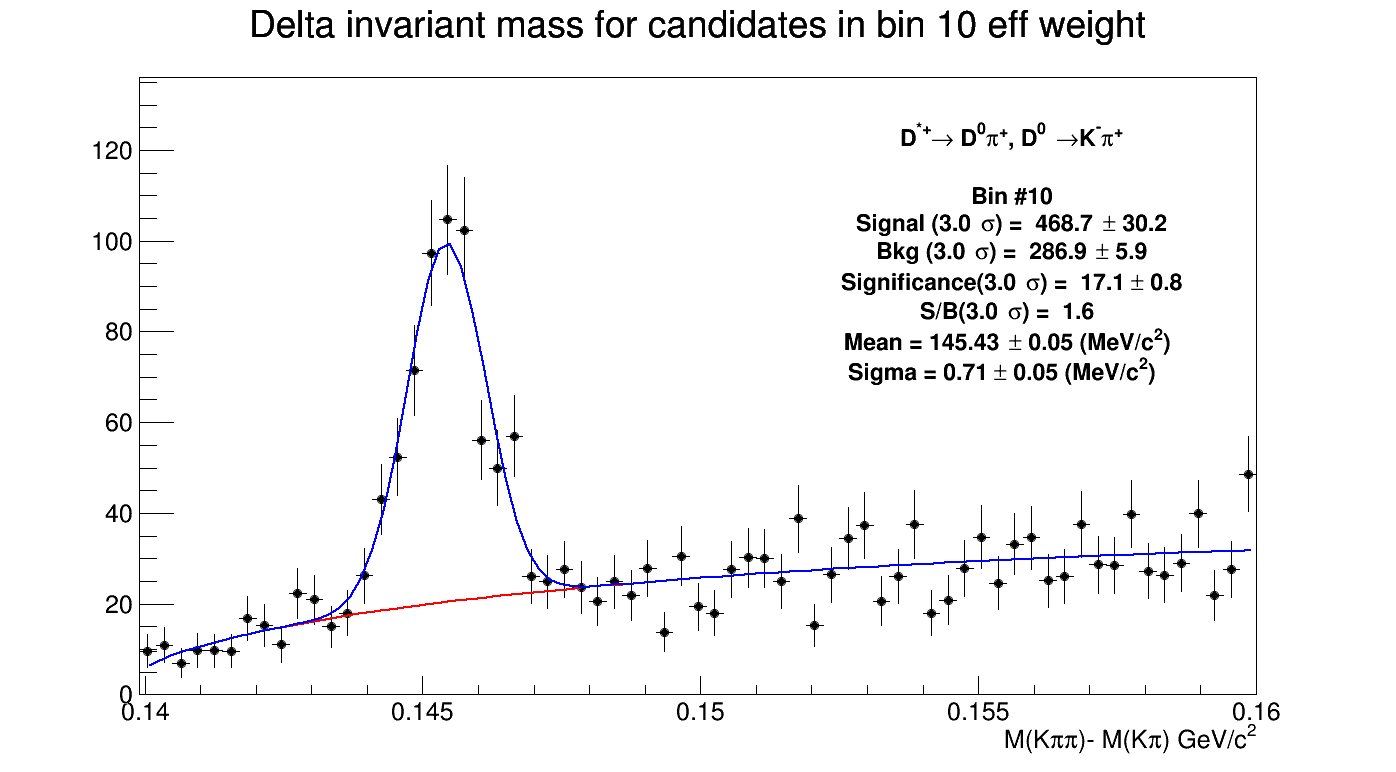
\includegraphics[width=0.6\linewidth, height=5.6cm]{figures/Dstar_wEFF/InvMassDistributions_Dstar_Bins10to10.png}}

\caption{Invariant mass distributions of $\Dstar$ corrected with efficiency in different $\text{p}_T$ regions. Top: $3< p_{T}^{\text{D}}< 4$ $\gev/c$ (left), $4< p_{T}^{\text{D}}< 5$ $\gev/c$ right), Mid 1: $5< p_{T}^{\text{D}}< 6$ $\gev/c$ (left), $6 < p_{T}^{\text{D}} < 7$ $\gev/c$ (middle), $7< p_{T}^{\text{D}}< 8$ $\gev/c$ (right); Mid2: $8< p_{T}^{\text{D}}< 10$ $\gev/c$, $10< p_{T}^{\text{D}}< 12$ $\gev/c$  (middle), $12 < p_{T}^{\text{D}}< 16$ $\gev/c$  (right) and Bottom: $16<p_{T}^{\text{D}}< 24$ $\gev/c$ .}
\label{fig:InvMassDs}
\end{figure}

\begin{figure}[!htp]
\centering
{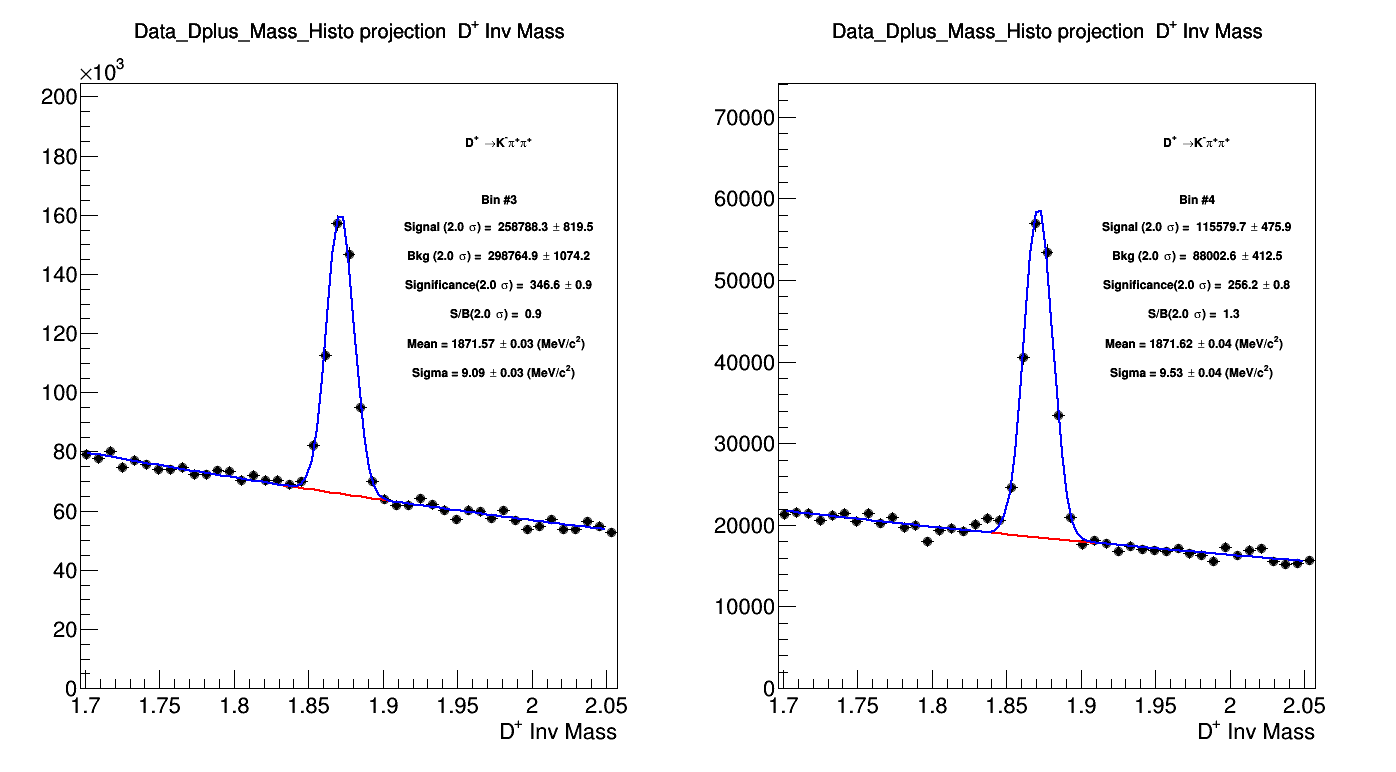
\includegraphics[width=1\linewidth, height=5.6cm]{figures/DplusPlotsweff/InvMassDistributions_Dplus_Bins3to4.png}}
{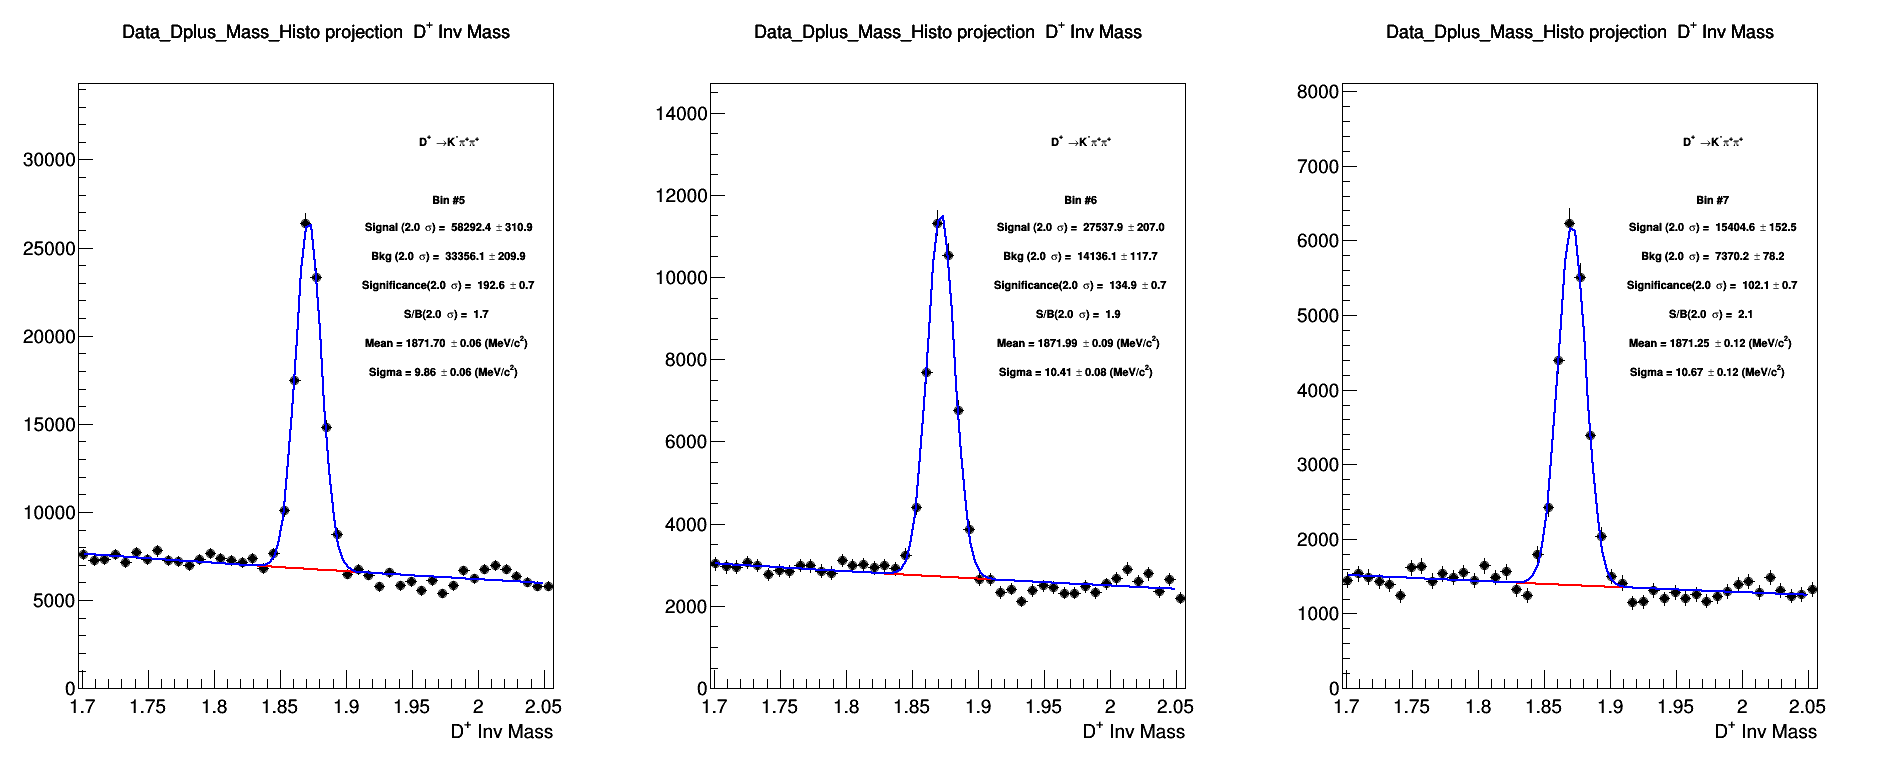
\includegraphics[width=1\linewidth, height=5.6cm]{figures/DplusPlotsweff/InvMassDistributions_Dplus_Bins5to7.png}}
{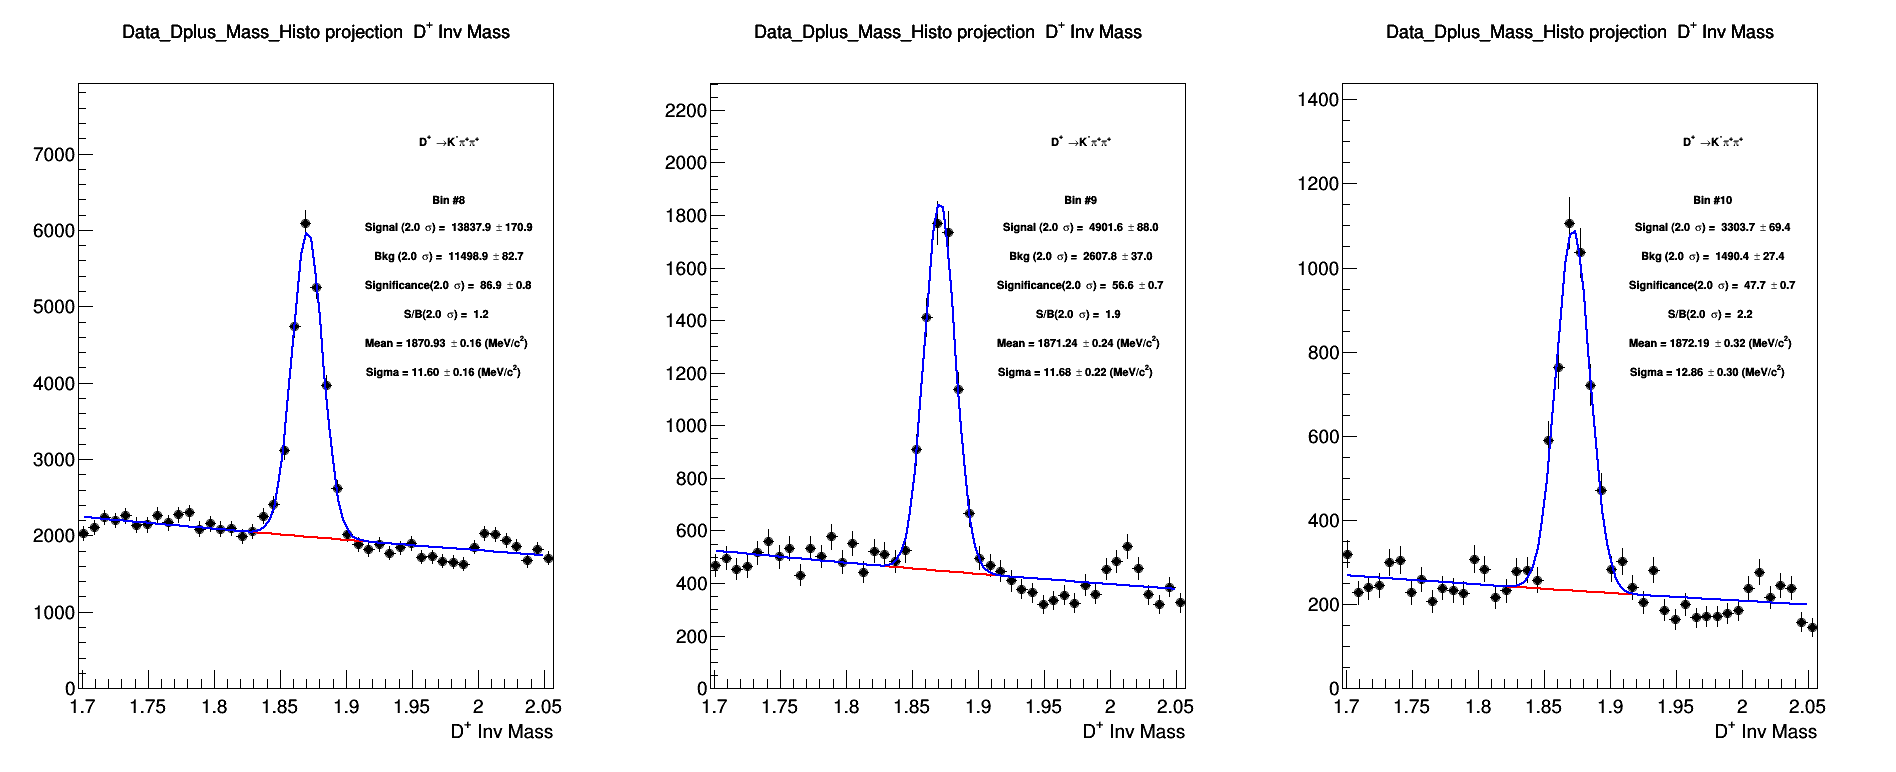
\includegraphics[width=1\linewidth, height=5.6cm]{figures/DplusPlotsweff/InvMassDistributions_Dplus_Bins8to10.png}}
{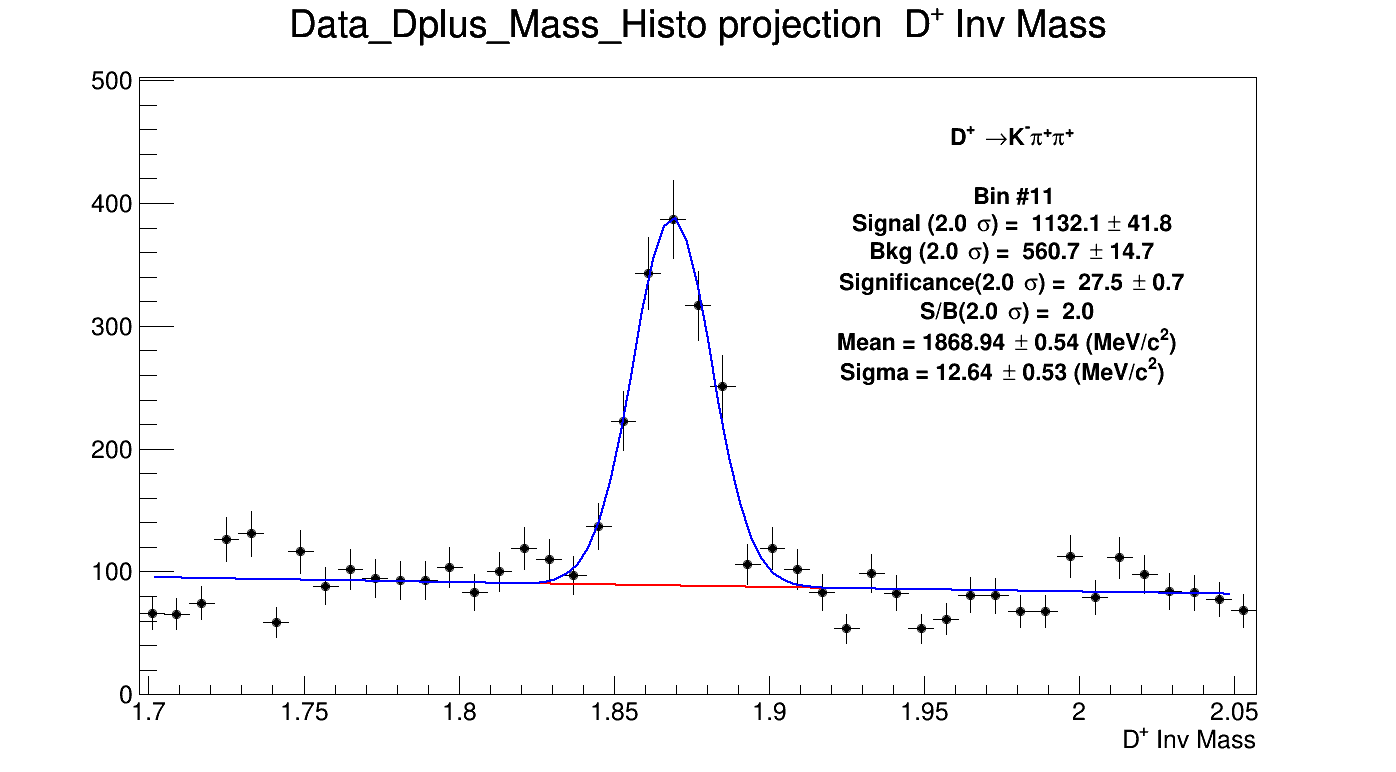
\includegraphics[width=0.6\linewidth, height=5.6cm]{figures/DplusPlotsweff/InvMassDistributions_Dplus_Bins11to11.png}}

\caption{Invariant mass distribution of $\Dplus$ corrected with efficiency in different $\text{p}_T$ regions. Top: $3< p_{T}^{\text{D}}< 4$ $\gev/c$ (left), $4< p_{T}^{\text{D}}< 5$ $\gev/c$ right), Mid 1: $5< p_{T}^{\text{D}}< 6$ $\gev/c$ (left), $6 < p_{T}^{\text{D}} < 7$ $\gev/c$ (middle), $7< p_{T}^{\text{D}}< 8$ $\gev/c$ (right); Mid2: $8< p_{T}^{\text{D}}< 10$ $\gev/c$, $10< p_{T}^{\text{D}}< 12$ $\gev/c$  (middle), $12 < p_{T}^{\text{D}}< 16$ $\gev/c$  (right) and Bottom: $16<p_{T}^{\text{D}}< 24$ $\gev/c$ .}
\label{fig:InvMassDp}
\end{figure}

For $\Dstar$, the standard D2H p-Pb cuts (for the 2013 cross section analysis, \cite{NoteD2HpPb}) were used. The same holds for the $\Dplus$, but with the addition of cuts on the normalized decay length in $xy$ plane and of the normalized difference between measured and expected daughter track impact parameters (topomatic cut).
A particular cut optimization was instead performed for the $\Dzero$ meson. Twelve cut sets were tried, with the goal of increasing the S/B factor, in order to reduce fluctuations induced by the sideband subraction (the limiting factor for the analysis performance).
In Figure \ref{fig:cutoptD0} the $\Dzero$-h correlation distributions are shown for the different cut sets, in exemplary kinematic regions (left column), together with the bin-by-bin relative statistical uncertainty on the data points (right column). The best cut set (option G) was defined from the standard cuts used for the p-Pb 2013 cross section analysis, with a tightened selection on the cosine of the pointing angle, and with the addition of a cut on the normalized decay length in $xy$ plane and of a selection on the normalized difference between measured and expected daughter track impact parameters (topomatic cut).

\begin{figure}[!htp]
\centering
{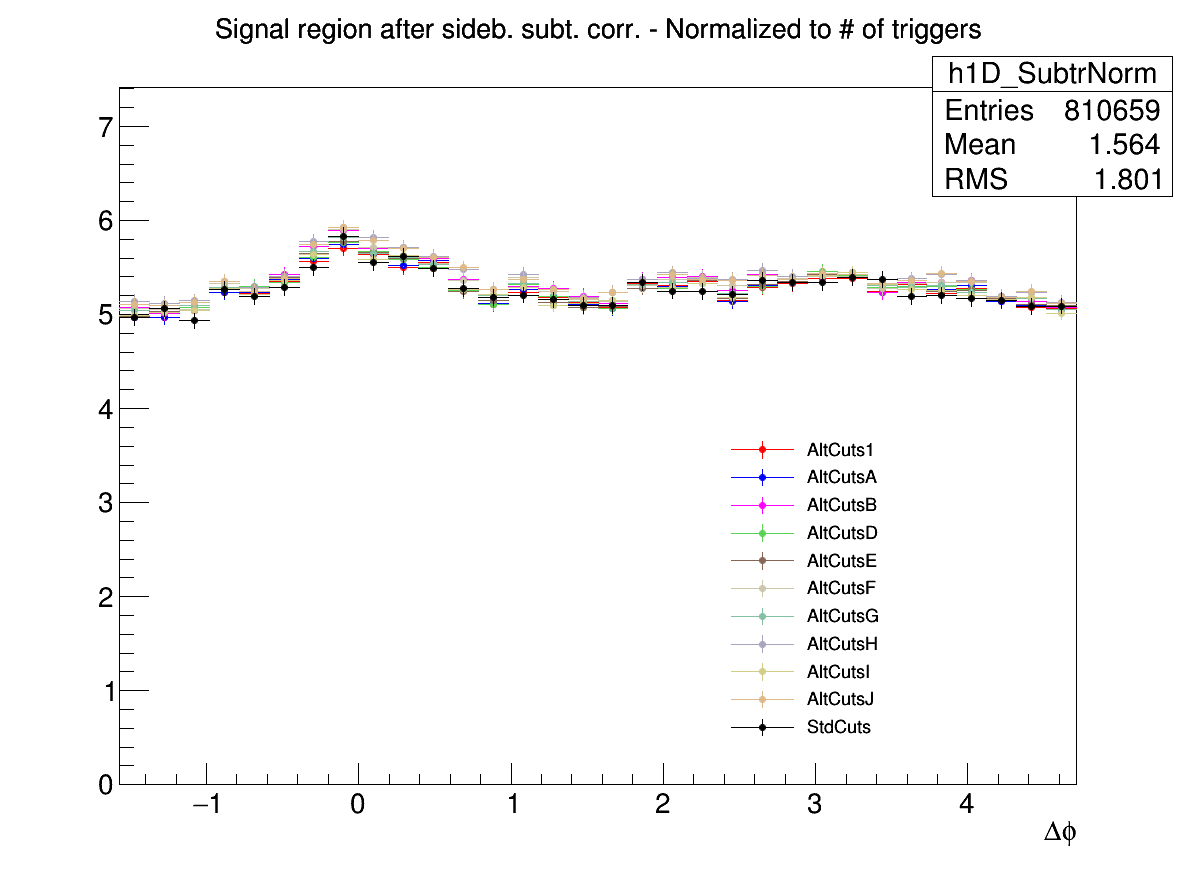
\includegraphics[width=0.47\linewidth, height=5.6cm]{figures/Cut_Optimiz_D0/AzimCorrDistr_Dzero_Canvas_PtIntBins3to5_PoolInt_thr03to99_Superimp.png}}
{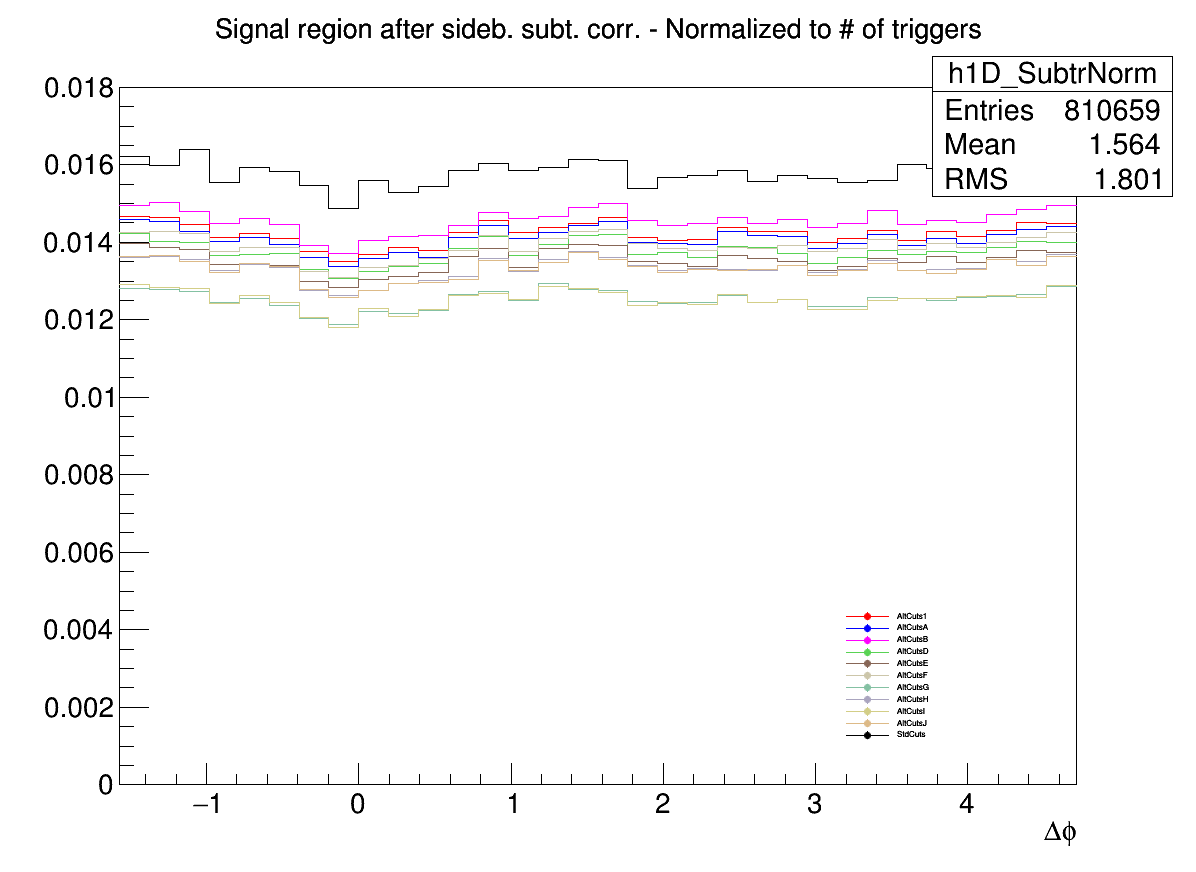
\includegraphics[width=0.47\linewidth, height=5.6cm]{figures/Cut_Optimiz_D0/Uncertanty_AzimCorrDistr_Dzero_Canvas_PtIntBins3to5_PoolInt_thr03to99.png}}
{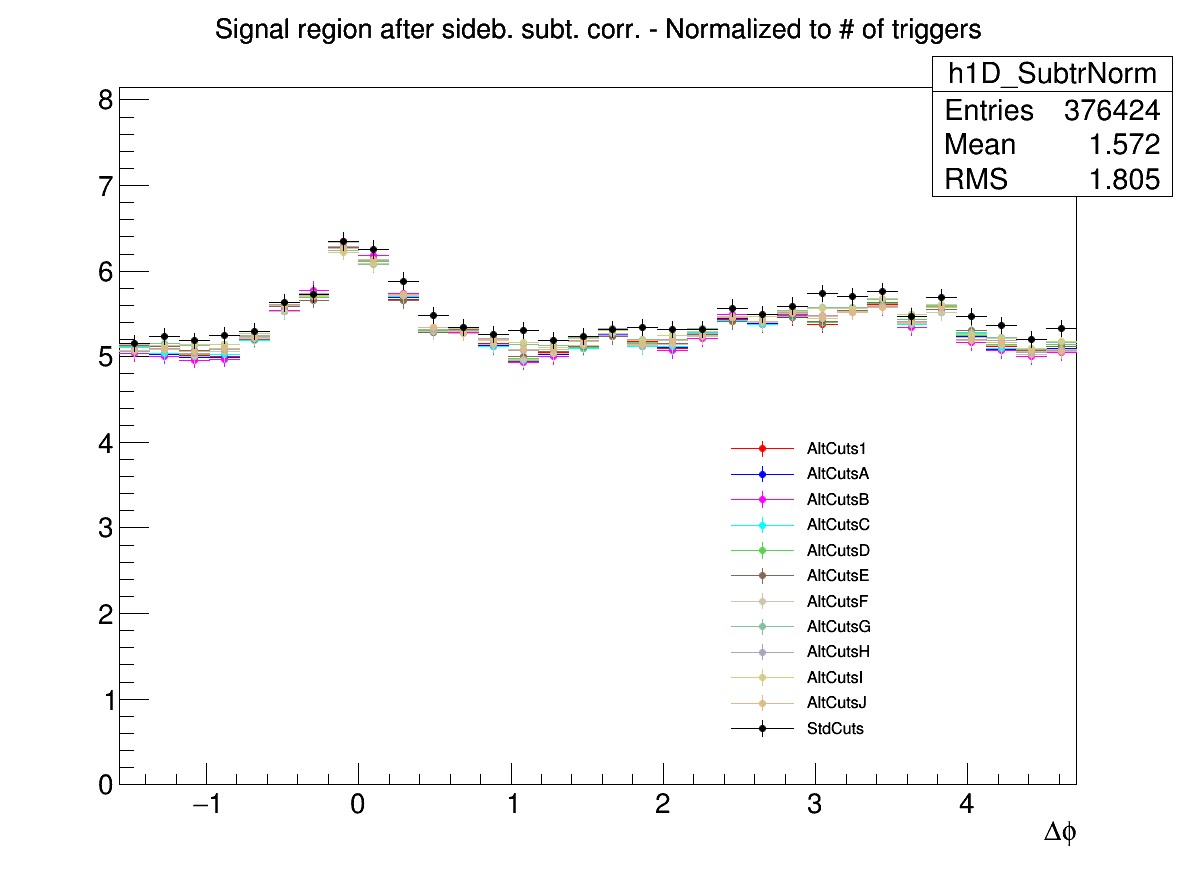
\includegraphics[width=0.47\linewidth, height=5.6cm]{figures/Cut_Optimiz_D0/AzimCorrDistr_Dzero_Canvas_PtIntBins6to8_PoolInt_thr03to99_Superimp.png}}
{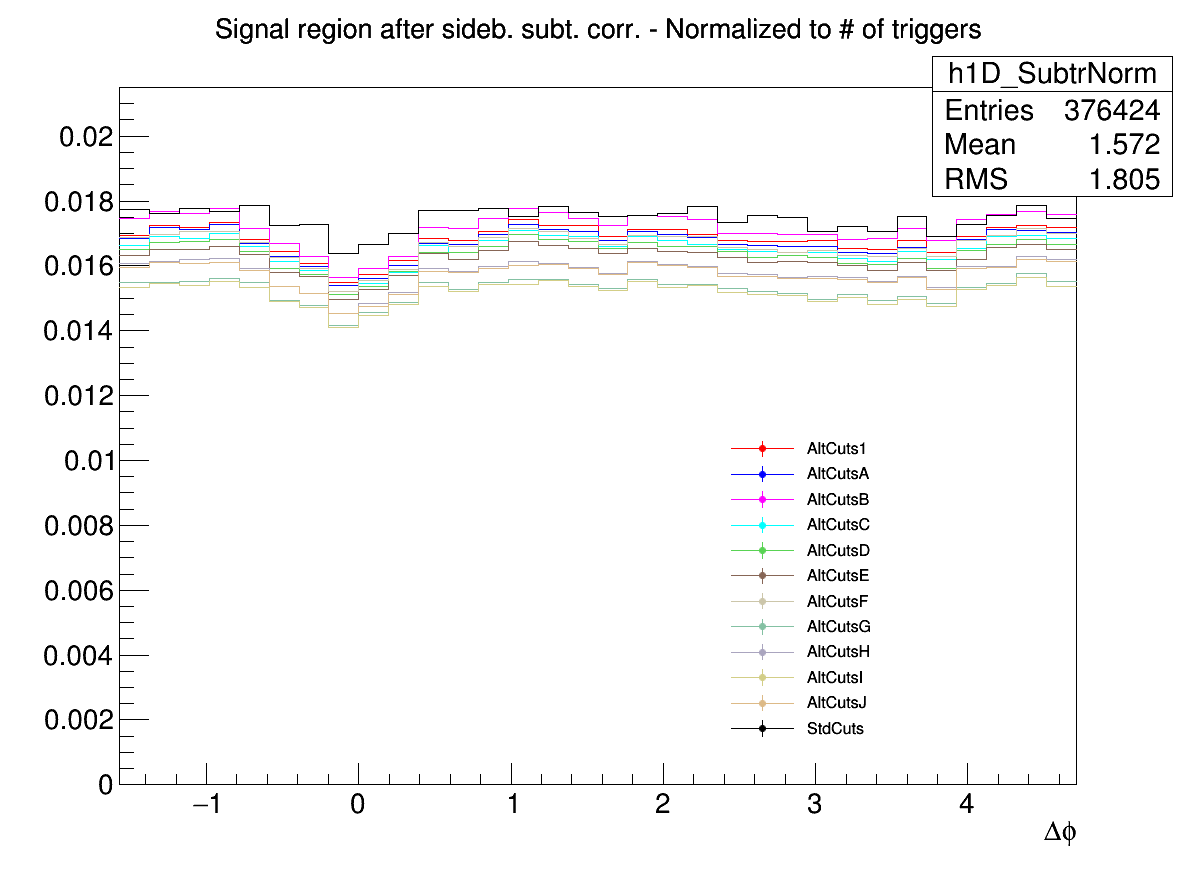
\includegraphics[width=0.47\linewidth, height=5.6cm]{figures/Cut_Optimiz_D0/Uncertanty_AzimCorrDistr_Dzero_Canvas_PtIntBins6to8_PoolInt_thr03to99.png}}
{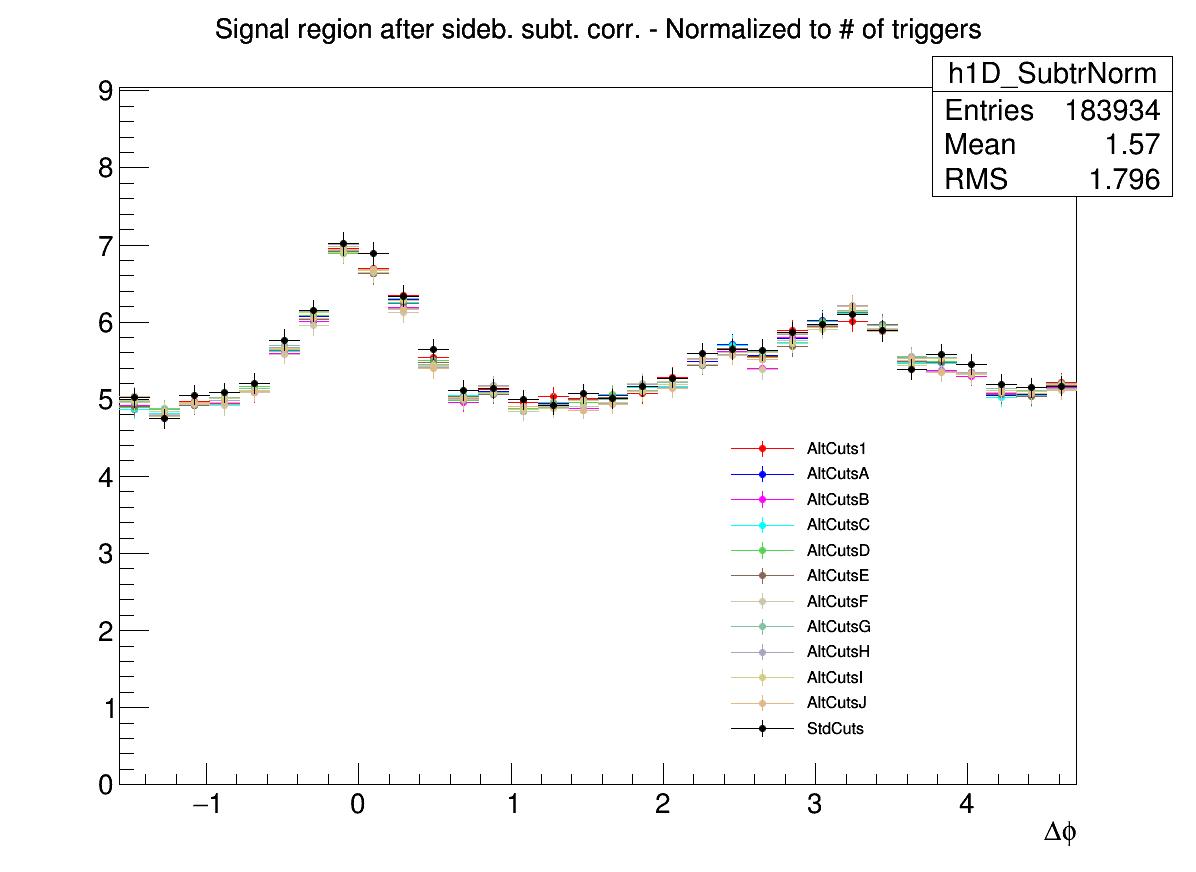
\includegraphics[width=0.47\linewidth, height=5.6cm]{figures/Cut_Optimiz_D0/AzimCorrDistr_Dzero_Canvas_PtIntBins9to10_PoolInt_thr03to99_Superimp.png}}
{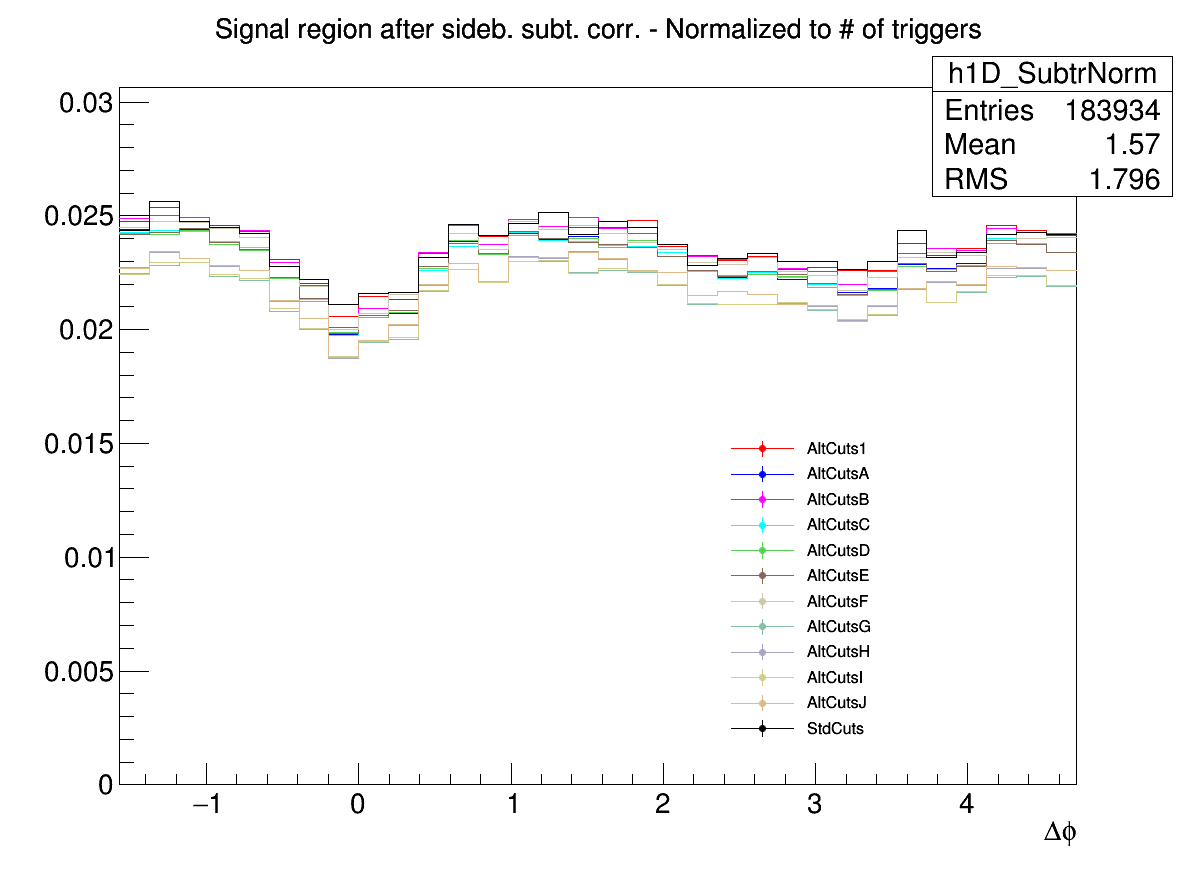
\includegraphics[width=0.47\linewidth, height=5.6cm]{figures/Cut_Optimiz_D0/Uncertanty_AzimCorrDistr_Dzero_Canvas_PtIntBins9to10_PoolInt_thr03to99.png}}

\caption{$\Dzero$-h correlation distributions with different cut options (left) and point-by-point relative statistical uncertainty (right) for $3< p_{T}^{\text{D}}< 5$ $\gev/c$ (top), $5< p_{T}^{\text{D}}< 8$ $\gev/c$ (middle), $8< p_{T}^{\text{D}}< 16$ $\gev/c$ (bottom), in all cases with associated track $\pt$ $> 0.3$ $\gev/c$.}
\label{fig:cutoptD0}
\end{figure}

\subsection{Code used for the analysis}
The code used for D meson-hadron correlation analysis is fully committed in AliPhysics. The analysis classes can be found in
\$ALICE\_ROOT/PWGHF/correlationHF/.  The  D meson specific classes where the aforementioned steps are carried out are
AliAnalysisTaskDStarCorrelations, AliAnalysisTaskSED0Correlations and AliAnalysisTaskDplusCorrelations. The classes which are common to the D meson specific analysis which includes the associated particle cuts and the correlation observables are AliHFAssociatedTrackCuts, AliHFCorrelator, AliHFOfflineCorrelator, AliReducedParticle and AliDhCorrelationExtraction. Several additional classes and macros in the same folder deal with the correction steps.

The final results presented here are extracted are the HFCJ pPb (n. 88) train runs 290-293 (for $\Dzero$ and $\Dplus$) and 286-289 (for $\Dstar$).

\subsection{Further details on corrections}
\subsubsection{Event Mixing}
The event-mixing technique is used for correcting the raw correlation distribution for effects arising
from the detector limited acceptance in rapidity and detector spatial inhomogeneities. The calculation of the Event
Mixing correlation distribution is performed online.%, following the strategy and the code developed for the \textit{PWGCF} correlation analyses. 
An event pool is created, where events preceding the one containing a D candidate are stored based on their properties (position of the vertex along the z axis and multiplicity). 
Each time a D meson candidate is found in an event, only the events contained in the same pool as the event under analysis is used to evaluate the correlations for the event mixing correction.% the correlation analysis on the mixed events is performed if the pool satisfies the conditions defined at its creation, being the same as described for the pp analysis (As well as the conditions for refreshing the pools).

The multiplicity and z vertex position bins for the pools used in the p-Pb analysis are the following:
\begin{itemize}
\item Multiplicity bins: $\left(0,40\right);\left(40,65\right);\left(65,+\infty\right)$
\item Vertex z $(cm)$ = $\left(-10,-2.5\right);\left(-2.5,2.5\right);\left(2.5,10\right)$
\end{itemize}
%(\ref{tab:em})


In an ideal case, the mixed event distribution is expected to have a constant flat distribution as function of $\Delta\phi$ and a triangular shaped distribution in $\Delta\eta$
deriving from the limited $\eta$ acceptance of the detector. The obtained distribution is used as a weight in each correlation bin, i.e, the corrected correlation distribution is calculated as follows:
\begin{equation}
\label{eq:mixing}
\frac{dN^{corr}\left(\Delta\phi \Delta\eta\right)}{d\Delta\phi d\Delta\eta} = \frac{\frac{dN^{SE}\left(\Delta\phi \Delta\eta\right)}{d\Delta\phi d\Delta\eta} }{\frac{dN^{ME}\left(\Delta\phi \Delta\eta\right)}{d\Delta\phi d\Delta\eta} }\frac{dN^{ME}\left(0,  0\right)}{d\Delta\phi d\Delta\eta}
\end{equation}
In the previous equation, the last term stands for the average of the bins in the region $-0.2 < \Delta\eta < 0.2$, $-0.2 < \Delta\phi < 0.2$ (multiple bins are used to minimize the effect of statistical fluctuations on the normalization of the mixed-event plots).

The mixed-event correlation distributions are built in both D meson signal and sideband regions. Both are
corrected with the relative distributions. An example of the mixed event distribution is shown in Fig.~\ref{fig:DplusSEbyMEPlots1} (middle panels). The expected triangular
shape in $\Delta\eta$ addresses the effect of the limited detector pseudo-rapidity acceptance. Note that the mixed-event distribution is limited to
the interval $\left|\Delta\eta\right|<1$: the decision to limit the mixed-event correction, and thus the whole analysis, to this range was taken in
order to avoid the so-called ``wing effect", i.e. the wing-like structures arising in the correlation distribution at large $\Delta\eta$ due to the
limited filling of the correlation bins in that region. The event mixing is calculated in the \textit{AliHFCorrelator} class and is computed in the same way for each D meson.


\begin{comment}
\begin{figure}[!ht]
\centering
%{\includegraphics[width=.95\linewidth]{figures/Dplus_low_dot5_SEbyME.png}}
 \caption{($\Delta \varphi , \Delta \eta$) correlation in the Sidebands and Signal region from Single Event and Mixing Event analysis for low $p_{T}$: $3 < p_{T}^{\text{D}^+} < 5 $\gev/c$$ with associated track $p_{T}$ threshold 0.3 $\gev/c$ }
\label{fig:DplusSEbyMEPlots1}
\end{figure}



\begin{figure}[!ht]
\centering
%Marianna
%{\includegraphics[width=.95\linewidth]{figures/Dplus_mid_dot5_SEbyME.png}}
 \caption{($\Delta \varphi , \Delta \eta$) correlation in the Sidebands and Signal region from Single Event and Mixing Event analysis for mid $p_{T}$: $5< p_{T}^{\text{D}^+}< 8 $\gev/c$$ with associated track $p_{T}$ threshold 0.3 $\gev/c$ }
\label{fig:DplusSEbyMEPlots2}
\end{figure}

\begin{figure}[!ht]
\centering
%{\includegraphics[width=.95\linewidth]{figures/Dplus_high_dot5_SEbyME.png}}
 \caption{($\Delta \varphi , \Delta \eta$) correlation in the Sidebands and Signal region from Single Event and Mixing Event analysis for high $p_{T}$: $8< p_{T}^{\text{D}^+}< 16 $\gev/c$$ with associcated track $p_{T}$ threshold 0.3 $\gev/c$ }
\label{fig:DplusSEbyMEPlots3}
\end{figure}

Figures \ref{fig:DplusSEbyMEPlots1}, \ref{fig:DplusSEbyMEPlots2}, \ref{fig:DplusSEbyMEPlots3} show the 2D correlation in Sideband Region and Signal region from SE and ME analysis for $D^+$ meson in different $p_{T}$ region.

\end{comment}

\newpage
\subsubsection{Tracking and D-meson trigger efficiency}

{\bf \normalsize (i) Tracking efficiency}: is calculated by obtaining the ratio between the yield at the reconstructed level and generated level, for a defined ``type" of particles (in our case non-identified particles) and it is estimated differentially in p$_T$, $\eta$, and z$_{vtx}$ of the event.\\
{\bf Implementation }: tracking efficiency maps are produced as TH3D histograms (p$_T$, $\eta$, z$_{vtx}$) obtained from MC analysis on the minimum-bias samples LHC17a2b$\_$fast and LHC17a2b$\_$cent$\_$woSDD, and applying at reconstructed level the track selections (summarized in Table.~\ref{table:effCuts}). These efficiency maps are used in the analysis tasks to extract single track efficiencies; each correlation pairs found in the data analysis is inserted in correlation plots with a weight of {\bf 1/efficiency value}. Example plots of the tracking efficiencies as a function of p$_T$ are shown in Fig.~\ref{fig:trackeff}.


%\begin{figure}[h]
%	\centering
%	\includegraphics[scale=0.35]{figures/pPb_STE_1D_pT_all_DCA.png}
%	\caption{Charged particle $p_T$ efficiency for different DCA values.}
%	\label{fig:trackeff}	
%\end{figure}


\begin{figure}[h]
	\centering
	%\includegraphics[scale=0.35]{figures/pPb_efficiencyVsspeicies.png}
	\caption{$p_T$ efficiency for standard track selection.}
	\label{fig:trackeffvsspecies}	
\end{figure}

\newpage
Details of cuts at event level and particle selection at different steps are listed in Table.~\ref{table:effCuts} . \\
\begin{table}[h]
\small
\centering % used for centering table

\begin{tabular}{  p{5cm} |  p{8.5cm} }
 \\
  \multirow{1}{*}{\large \textbf {MC Generated }} \\
\hline
\\
     Stages         &              Cuts \\
\hline\hline & \\		            	
  1.MC Part with Generated Cuts         &    {\textbf {After Event Selection}}\\
																		   & Charge\\
																		    & PDG Code\\
														  				  & Physical Primary \\

   2. MC Part with Kine Cuts         &              {\textbf {Kinematics Cuts }}\\
															    & -0.8$\textless \eta \textless  0.8$\\
															    & pT $\textgreater$ 0.3 (GeV/$c$)\\

&		\\            	


\multirow{1}{*}{\large \textbf {MC Reconstructed }} & \\
\hline


\hline & \\		            	                        	
4. Reco tracks        &                             {\textbf {After Event Selection}}\\
															   & Physical Primary \\
															
															
5. Reco tracks with Kine Cuts         &               {\textbf  {Kinematics Cuts }}\\
															    & -0.8$\textless \eta \textless  0.8$\\
															    & pT $\textgreater$ 0.3 (GeV/$c$)\\



6. MC true with Quality Cuts         &      			      {\textbf  {Quality Cuts }} \\
																	&SetRequireSigmaToVertex(kFALSE) \\
																	&SetDCAToVertex2D(kFALSE) \\
																	&SetMinNCrossedRowsTPC(70)\\
																	&SetMinRatioCrossedRowsOverFindableClustersTPC(0.8)\\
																	&SetMinNClustersITS(3)\\
																	&SetMaxChi2PerClusterTPC(4)\\
																	&SetMaxDCAToVertexZ(1) \\
																	&SetMaxDCAToVertexXY(0.25) \\
																	&SetRequireTPCRefit(TRUE) \\
																	&SetRequireITSRefit(FALSE) \\

7. Reco tracks with Quality Cuts         &             {\textbf  {Same as step 6}} \\

 &\\		            	            		

 \hline \hline
 \\
\end{tabular}
\caption{\large {Single Track Efficiency cuts detail}} % title of Table
\label{table:effCuts}	
\end{table}


{\bf \large (ii) D Meson efficiency} - Due to limited statistics, the correlation analysis is performed in quite wide p$_\mathrm{T}$ bins and in each of them the reconstruction and selection efficiency of D mesons is not flat (Fig.~\ref{fig:dpluseff},~\ref{fig:d0eff}), in particular in the lower $\pt$ region. We correct for the p$_\mathrm{T}$ dependence of the trigger efficiency within each p$_\mathrm{T}$-bin.
This correction is applied online, by using a map of D meson efficiency as a function of p$_\mathrm{T}$ and event multiplicity (in terms of SPD tracklets in $|\eta|<1$) extracted from the enriched Monte Carlo sample LHC17d2a$\_$fast$\_$new.
While running the analysis, each correlation entry is weighted by {\bf 1/trigger efficiency}. It was observed that multiplicity dependence of the efficiency does not bias the extraction of the signal yield from the invariant mass distributions (which, as anticipated, are also weighted in the same manner). Efficiency plots for $\Dzero$, $\Dplus$ and $\Dstar$ mesons are shown in Fig.~\ref{fig:doeff}, Fig.~\ref{fig:dpluseff} and ~\ref{fig:dstareff}.

\begin{figure}[!htp]
	\centering
%Marianna
	%\includegraphics[width=.48\linewidth]{figures/D0Eff_From_c_wLimAcc_2D_pPb.png}  % by Fabio
	%\includegraphics[width=.48\linewidth]{figures/D0Eff_From_c_wLimAcc_1D_pPb.png} \\
	%\includegraphics[width=.30\linewidth]{figures/D0Eff_ProjMult_3to4GeV.png}
	%\includegraphics[width=.30\linewidth]{figures/D0Eff_ProjMult_5to6GeV.png}
	%\includegraphics[width=.30\linewidth]{figures/D0Eff_ProjMult_8to12GeV.png}
\caption{Top panel: (p$_\mathrm{T}$, multiplicity) dependence (left) and p$_T$ dependence (right) of prompt $D^0$ meson efficiency. Bottom panels: multiplicity dependence of $D^0$ meson efficiency for three $D^0$ p$_\mathrm{T}$ ranges: 3-4 GeV/$c$ (left), 5-6 GeV/$c$ (center), 8-12 GeV/$c$ (right). For tracklet multiplicity$>$ 120, due to the limited statistics, the efficiency value is fixed to the one obtained for 90$<$tracklet multiplicity$<$120.	
	\label{fig:d0eff}	
\end{figure}

\begin{figure}[h]
	\centering
	%Marianna
	%\includegraphics[width=.50\linewidth]{figures/Efficiency_Dplus_Corrected_Central.png} \\% by Jitendra
	%\includegraphics[width=.30\linewidth]{figures/Dplus_3_5Multplicty_eff.png}
	%\includegraphics[width=.30\linewidth]{figures/Dplus_5_8Multplicty_eff.png}
	%\includegraphics[width=.30\linewidth]{figures/Dplus_8_16Multplicty_eff.png}
	\caption{Top panel: (p$_T$, multiplicity) dependence of $D^+$ meson efficiency. Bottom panels: $D^+$ meson efficiency in multiplicity for three $D^+$ p$_\mathrm{T}$ranges: 3-5 GeV/$c$ (left), 5-8 GeV/$c$ (center), 8-16 GeV/$c$ (right).}
	\label{fig:dpluseff}	
\end{figure}

\begin{figure}[!htp]
	\centering
%Marianna
	%\includegraphics[width=.48\linewidth]{figures/D0Eff_From_c_wLimAcc_2D_pPb.png}  % by Fabio
	%\includegraphics[width=.48\linewidth]{figures/D0Eff_From_c_wLimAcc_1D_pPb.png} \\
	%\includegraphics[width=.30\linewidth]{figures/D0Eff_ProjMult_3to4GeV.png}
	%\includegraphics[width=.30\linewidth]{figures/D0Eff_ProjMult_5to6GeV.png}
	%\includegraphics[width=.30\linewidth]{figures/D0Eff_ProjMult_8to12GeV.png}
\caption{Top panel: (p$_\mathrm{T}$, multiplicity) dependence (left) and p$_T$ dependence (right) of prompt $\Dstar$ meson efficiency. Bottom panels: multiplicity dependence of $\Dstar$ meson efficiency for three $\Dstar$ p$_\mathrm{T}$ ranges: 3-4 GeV/$c$ (left), 5-6 GeV/$c$ (center), 8-12 GeV/$c$ (right). For tracklet multiplicity$>$ 120, due to the limited statistics, the efficiency value is fixed to the one obtained for 90$<$tracklet multiplicity$<$120.}
	\label{fig:dstareff}	
\end{figure}
\newpage 

\subsubsection{Correction for bias on B to D decay topologies}
\label{MCclosure}
To verify the consistency of the analysis chain and of the corrections applied to the  correlation distributions extracted from data, a Monte Carlo closure test was developed and tried on the $\Dzero$-h analysis.

On the Monte Carlo enriched with charm and beauty quarks (LHC17d2a$\_$fast$\_$new), the correlation analysis was performed both at kinematic level and at reconstructed level. At kinematic level, only acceptance cuts were applied on the D mesons and the associated particles, using the Monte Carlo information for the identification of the D mesons and the hadrons in the event and rejecting the non-primary particles. At reconstructed level, the analysis was performed as if it were executed on data, applying the event selection, the acceptance cuts for D mesons and the associated particles, selecting the D meson candidates with filtering cuts on their daughters, topological cuts and PID selection, and then keeping only the true D mesons by looking at the Monte Carlo truth; non-primary particles were rejected by means of the DCA selection. Event mixing correction was applied both at reconstructed and at kinematic level, where it takes into account just the effects of the acceptance cuts. In addition, at reconstructed level also tracking efficiency and trigger efficiency correction were applied.

Examples of correlation plots at both steps are shown in Figure~\ref{fig:MC_Kine} and~\ref{fig:MC_Reco}, separating the contribution of associated tracks and D mesons from different origins to the correlation distribution, as described in the legend of the plots.

\clearpage
\begin{figure}
{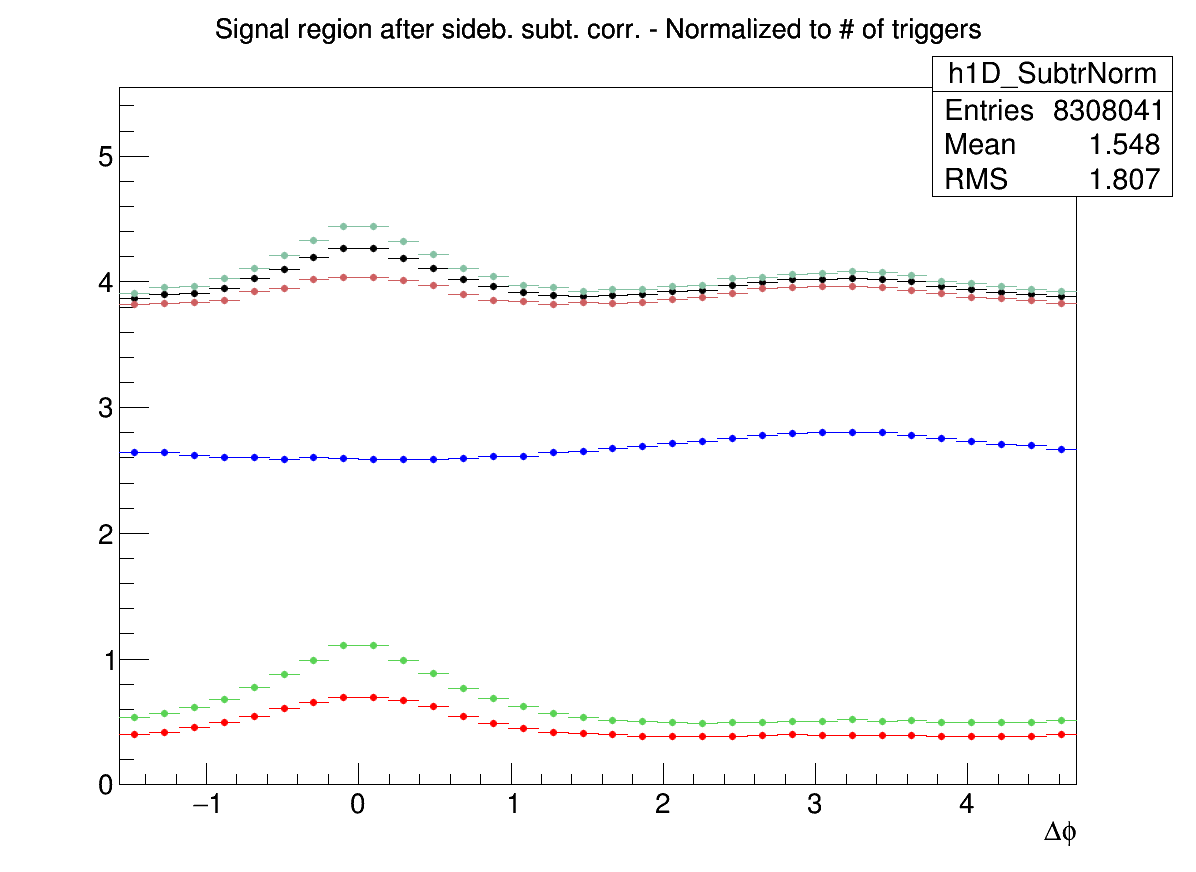
\includegraphics[width=.48\linewidth]{figures/MC_closure/AzimCorrDistr_Dzero_Canvas_PtIntBins4to5_PoolInt_thr03to1_Superimposed_Kine.png}}
{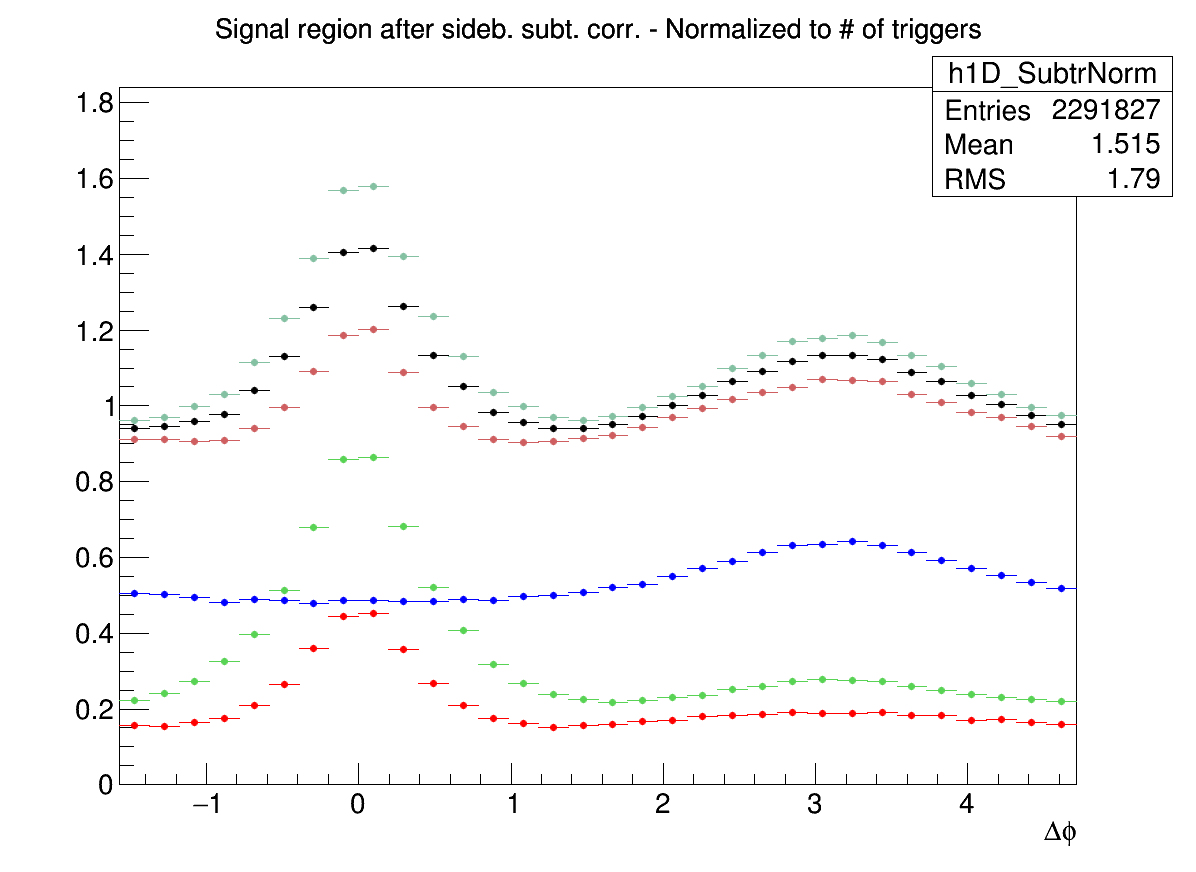
\includegraphics[width=.48\linewidth]{figures/MC_closure/AzimCorrDistr_Dzero_Canvas_PtIntBins4to5_PoolInt_thr1to99_Superimposed_Kine.png}} \\
{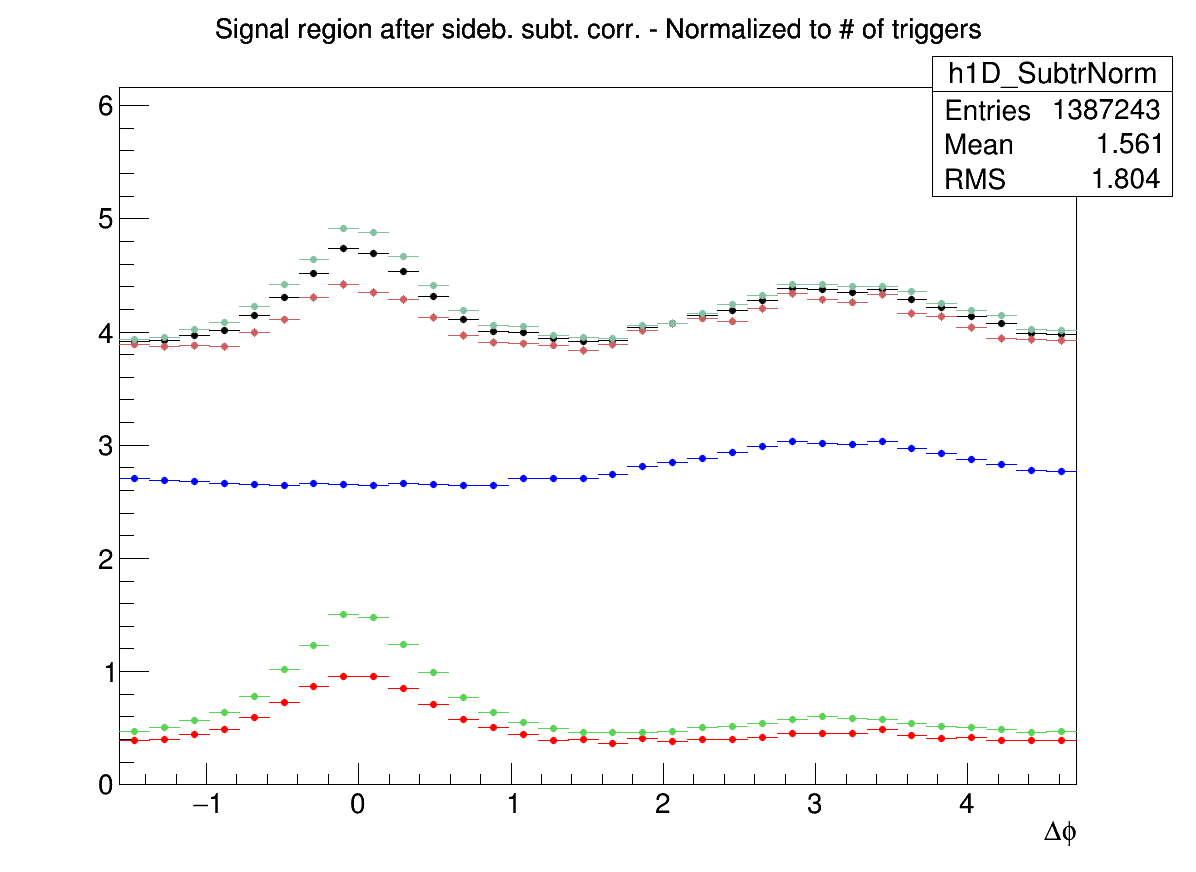
\includegraphics[width=.48\linewidth]{figures/MC_closure/AzimCorrDistr_Dzero_Canvas_PtIntBins9to10_PoolInt_thr03to1_Superimposed_Kine.png}}
{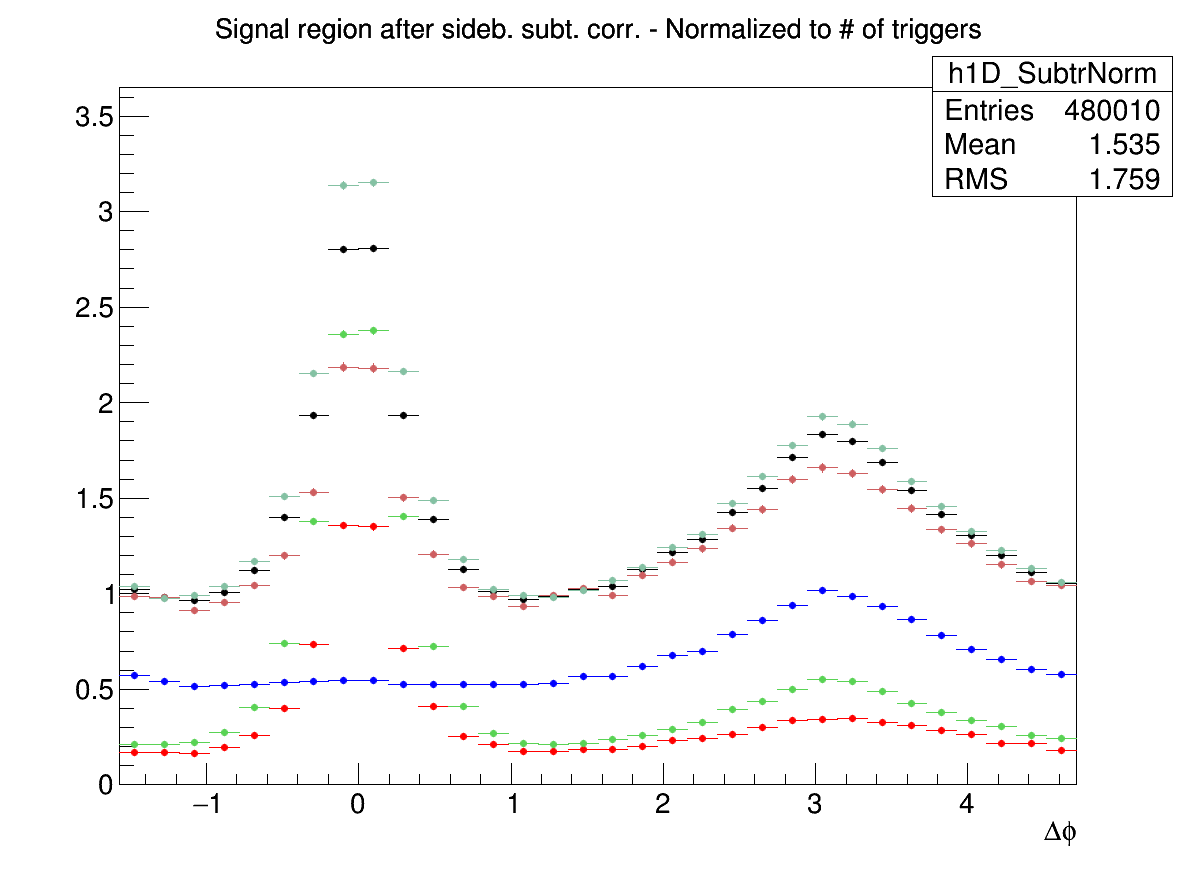
\includegraphics[width=.48\linewidth]{figures/MC_closure/AzimCorrDistr_Dzero_Canvas_PtIntBins9to10_PoolInt_thr1to99_Superimposed_Kine.png}}
\caption{$D^0$-hadrons azimuthal correlation distribution obtained from Monte Carlo, at kinematic step. Black points: All $D^0$-all hadrons, normalized by all $D^0$ triggers; light red points: $D^0$ from c-hadrons from c, normalized by c-$D^0$ triggers; dark red points: $D^0$ from c-all hadrons, normalized by c-$D^0$ triggers; light green points: $D^0$ from b-hadrons from b, normalized by b-$D^0$ triggers; dark green points: $D^0$ from b-all hadrons, normalized by b-$D^0$ triggers; blue points: All $D^0$-hadrons from light quarks, normalized by all $D^0$ triggers.
The panels show the ranges: $3 < \pt$(D)$ < 5$ GeV/c, $0.3 < \pt$(assoc)$ < 1$ GeV/c (top-left); $3 < \pt$(D)$ < 5$ GeV/c, $\pt$(assoc)$ > 1$ GeV/c (top-right); $8 < \pt$(D)$ < 16$ GeV/c, $0.3 < \pt$(assoc)$ < 1$ GeV/c (bottom-left); $8 < \pt$(D)$ < 16$ GeV/c, $\pt$(assoc)$ > 1$ GeV/c (bottom-right).}
\label{fig:MC_Kine}
\end{figure}

\begin{figure}
{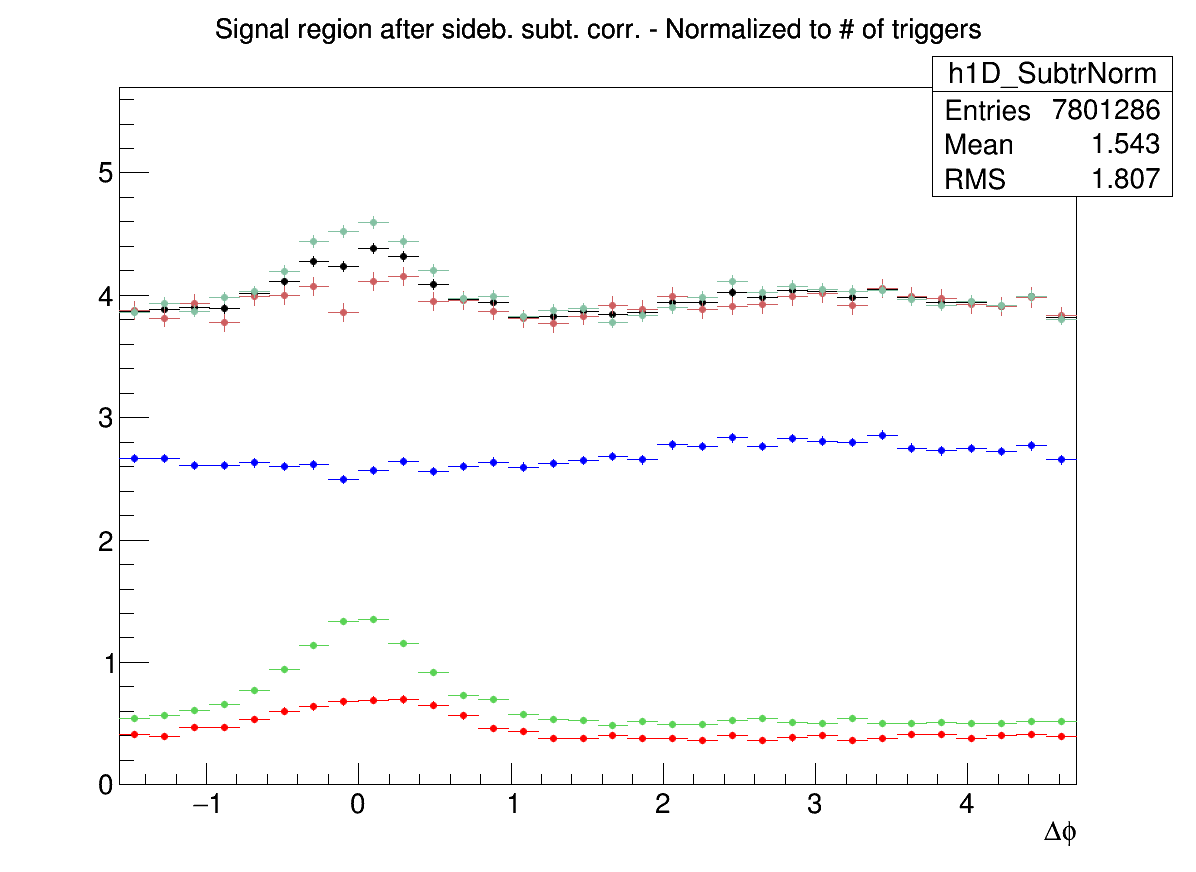
\includegraphics[width=.48\linewidth]{figures/MC_closure/AzimCorrDistr_Dzero_Canvas_PtIntBins4to5_PoolInt_thr03to1_Superimposed_Reco.png}}
{\includegraphics[width=.48\linewidth]{figures/MC_closure/AzimCorrDistr_Dzero_Canvas_PtIntBins4to5_PoolInt_thr1to99_Superimposed_Reco.png}} \\
{\includegraphics[width=.48\linewidth]{figures/MC_closure/AzimCorrDistr_Dzero_Canvas_PtIntBins9to10_PoolInt_thr03to1_Superimposed_Reco.png}}
{\includegraphics[width=.48\linewidth]{figures/MC_closure/AzimCorrDistr_Dzero_Canvas_PtIntBins9to10_PoolInt_thr1to99_Superimposed_Reco.png}}
\caption{$D^0$-hadrons azimuthal correlation distribution obtained from Monte Carlo, at reconstructed step. Black points: All $D^0$-all hadrons, normalized by all $D^0$ triggers; light red points: $D^0$ from c-hadrons from c, normalized by c-$D^0$ triggers; dark red points: $D^0$ from c-all hadrons, normalized by c-$D^0$ triggers; light green points: $D^0$ from b-hadrons from b, normalized by b-$D^0$ triggers; dark green points: $D^0$ from b-all hadrons, normalized by b-$D^0$ triggers; blue points: All $D^0$-hadrons from light quarks, normalized by all $D^0$ triggers.
The panels show the ranges: $3 < \pt$(D)$ < 5$ GeV/c, $0.3 < \pt$(assoc)$ < 1$ GeV/c (top-left); $3 < \pt$(D)$ < 5$ GeV/c, $\pt$(assoc)$ > 1$ GeV/c (top-right); $8 < \pt$(D)$ < 16$ GeV/c, $0.3 < \pt$(assoc)$ < 1$ GeV/c (bottom-left); $8 < \pt$(D)$ < 16$ GeV/c, $\pt$(assoc)$ > 1$ GeV/c (bottom-right).}
\label{fig:MC_Reco}
\end{figure}

The consistency check we performed was to verify whether, after having applied all the corrections to the azimuthal correlation plots at reconstructed level, the results were compatible with the ones at kinematic level. Hence, the ratios of fully corrected reconstructed plots over kinematic plots were evaluated in all the $D^0$ $p_\text{T}$ bins and for the various $p_\text{T}$ thresholds for the associated tracks, separating the contributions for the different origins of particles and triggers. The ratios, shown in Figure~\ref{fig:MC_Ratios}, denote a good compatibility with 1, within the uncertainties, apart from {\bf slight divergencies of the average value of the ratio at higher associated track $\pt$ ranges, of about 3\% (value introduced as a systematic uncertainty flat in $\Delta\phi$), and} some structures in the near side region for the beauty origin case.
These structures were already found in the pp 2010 and p-Pb 2013 analysis, and it was verified that they are induced our topological selection for the D mesons. Indeed, in cases in which the D meson triggers come from B hadrons, applying the topological cuts (especially the cosine of the pointing angle) tends to favour cases with a small angular opening between the products of the B hadron decay (i.e. the D meson trigger itself and other particles), with respect to cases where the B decay particles are less collinear.

\begin{figure}
\centering
{\includegraphics[width=.48\linewidth]{figures/MC_closure/MCClosure_Dzero_Canvas_PtIntBins4to5_PoolInt_thr03to1.png}}
{\includegraphics[width=.48\linewidth]{figures/MC_closure/MCClosure_Dzero_Canvas_PtIntBins4to5_PoolInt_thr1to99.png}} \\
{\includegraphics[width=.48\linewidth]{figures/MC_closure/MCClosure_Dzero_Canvas_PtIntBins9to10_PoolInt_thr03to1.png}}
{\includegraphics[width=.48\linewidth]{figures/MC_closure/MCClosure_Dzero_Canvas_PtIntBins9to10_PoolInt_thr1to99.png}}
\caption{Ratios of fully corrected azimuthal correlation plots at reconstructed level over azimuthal correlation plots at kinematic level, in the two $D^0$ $p_\text{T}$ bins, for the different associated $p_\text{T}$ ranges. Black points: All $D^0$-all hadrons, normalized by all $D^0$ triggers; light red points: $D^0$ from c-hadrons from c, normalized by c-$D^0$ triggers; dark red points: $D^0$ from c-all hadrons, normalized by c-$D^0$ triggers; light green points: $D^0$ from b-hadrons from b, normalized by b-$D^0$ triggers; dark green points: $D^0$ from b-all hadrons, normalized by b-$D^0$ triggers; blue points: All $D^0$-hadrons from light quarks, normalized by all $D^0$ triggers.
The panels show the ranges: $3 < \pt$(D)$ < 5$ GeV/c, $0.3 < \pt$(assoc)$ < 1$ GeV/c (top-left); $3 < \pt$(D)$ < 5$ GeV/c, $\pt$(assoc)$ > 1$ GeV/c (top-right); $8 < \pt$(D)$ < 16$ GeV/c, $0.3 < \pt$(assoc)$ < 1$ GeV/c (bottom-left); $8 < \pt$(D)$ < 16$ GeV/c, $\pt$(assoc)$ > 1$ GeV/c (bottom-right).}
\label{fig:MC_Ratios}
\end{figure}

In the Monte Carlo closure test, this situation is reflected in the correlation distributions at reconstructed level, where the topological selection is applied, while it does not occur at kinematic level. Hence, in the reconstructed/kinematic ratio, the distribution would show an excess for $\Delta\varphi = 0$ (due to the favoured decays with small opening angle), which is then compensated by a depletion for larger values of $\Delta\varphi = 0$ (corresponding to B decays with larger angles, which are disfavoured).
These structures are prominent at low $D^0$ $p_\text{T}$, where the topological cuts are tighter, and tend to disappear at higher $\pt$, where the selections are released. They are also larger in the higher associated track $\pt$ ranges, where the fraction of B-hadron decay tracks dominate the overall correlation distributions.

The data correlation distribution need to be corrected for this bias, and in particular for the enhancement of b-origin correlation pairs at the centre of the near side region, which would influence the near-side peak features.
In order to do this, the amount of the b-origin excess is evaluated from the Reco/Kine ratio, by considering the b-$\Dzero$-all tracks case (dark green points). The excess at Reco level (affecting data) is quantified as a $\Delta\phi$ modulation for the three points an each side of the $\Delta\phi = 0$ value. This is done separately in each $\pt$ range.
Then, the correction is done by applying this modulation to the data correlation distributions, but taking into account that only the correlation entries from B$\rightarrow$D are affected, while the c$\rightarrow$D correlations need to be left unaltered.
On data, the B$\rightarrow$D correlation pairs are a fraction (1-$\fprompt$) of the total.
In addition, the amplitude of B$\rightarrow$D correlation pattern with respect to the overall correlation distributions is:
\begin{equation}
\frac{{\rm B}\rightarrow{\rm D}_{\rm amplitude}}{({\rm B+c})\rightarrow{\rm D}_{\rm amplitude}} = \frac{{\rm B}\rightarrow{\rm D}_{\rm amplitude}}{{\rm B}\rightarrow{\rm D}_{\rm amplitude} \cdot (1-\fprompt) + {\rm c}\rightarrow{\rm D}_{\rm amplitude} \cdot \fprompt}
\end{equation}
where the two amplitudes are evaluated from the Monte Carlo distributions of Figure \ref{fig:MC_Reco}, and $\fprompt$ with the procedure described in \ref{feeddown}
To account for these features, and have the correction applied only on the B$\rightarrow$D correlations, the modulations extracted by the Reco/Kine ratios are thus rescaled by the factor:
\begin{equation}
(1 - \fprompt) \cdot \frac{{\rm B}\rightarrow{\rm D}_{\rm amplitude}}{{\rm B}\rightarrow{\rm D}_{\rm amplitude} \cdot (1-\fprompt) + {\rm c}\rightarrow{\rm D}_{\rm amplitude} \cdot \fprompt}
\end{equation}
before being applied to the data points. The effect of the correction is a downward shift of the data points in the near-side region. The maximum value of the shift is of 8\%, at the centre of the near-side peak, for the lowest D-meson $\pt$ range ($5 < \pt < 8$ GeV/c) and the highest associated track $\pt$ range ($\pt > 3$ GeV/c). The typical values are instead of a couple of percentage points. The correction is zero in the highest D-meson $\pt$ range.
To take into account for possible inaccuracies in the definition of the modulations, or in their rescaling, a systematic uncertainty is  applied on the corrected data points (as described in the related section).

\clearpage
%\end{document}


\subsubsection{Secondary track contamination}
\label{secondaries}
The secondary tracks inside the associated track sample, due to interaction of primary track with the detector material or to decays of strange hadrons, are mostly removed by the DCA cuts applied during the cut selection pahse (DCA($xy$)<1 cm, DCA($z$)<1 cm).
Anyway, a small fraction of secondary tracks survives this cut, and the data correlation distributions have to be corrected for this residual contamination.
The fraction of surviving secondary tracks is evaluated via a study on the LHC17d2a$\_$fast$\_$new sample, by counting the number of tracks accepted by the selection whose corresponding generated-level track doesn't satisfy the IsPhysicalPrimary() call, and dividing this number by the total numner of accepted tracks.
The outcome of the check is reported in Figure \ref{fig:secnumber}. As it's visible, no more than 5\% secondary tracks pass the selection. Moreover, the fraction of residual secondary tracks is flat along the $\Delta\phi$ axis, as shown, for exemplary $\pt$ regions, in Figure \ref{fig:secdPhi}, where the inhomogeneities are always below 1\%.
For this reason, it is possible to directly scale the data correlation distributions by their purity fraction (i.e. 1 - secondary contamination). This is done with an associated $\pt$ dependence, due to the increase of the purity with the track $\pt$, while the purity fraction is taken flat versus the D-meson $\pt$.

\begin{figure}[h]   %da B
	\centering
	%Marianna
		  % by Fabio
	\includegraphics[width=.48\linewidth]{figures/SecTracks/FractOfSecOverTotal_3to5.png}
	\includegraphics[width=.48\linewidth]{figures/SecTracks/FractOfSecOverTotal_5to8.png}
    \includegraphics[width=.48\linewidth]{figures/SecTracks/FractOfSecOverTotal_8to16.png}
    \includegraphics[width=.48\linewidth]{figures/SecTracks/FractOfSecOverTotal_16to24.png}
	\caption{Fraction of secondary tracks over total amount of tracks which pass the DCA selection. The four panel show the fractions for the D-meson $\pt$ ranges: 3-5, 5-8, 8-16, 16-24, respectively. Inside each panel, the associated track $\pt$ ranges are shown on the $x$-axis.}
	\label{fig:secnumber}	
\end{figure}

\begin{figure}[h]   %da B
	\centering
	%Marianna
		  % by Fabio
	\includegraphics[width=.48\linewidth]{figures/SecTracks/DeltaPhi_3to5_03to99_RatioSecOverAll.png}
	\includegraphics[width=.48\linewidth]{figures/SecTracks/DeltaPhi_5to8_03to99_RatioSecOverAll.png}
    \includegraphics[width=.48\linewidth]{figures/SecTracks/DeltaPhi_8to16_03to99_RatioSecOverAll.png}
    \includegraphics[width=.48\linewidth]{figures/SecTracks/DeltaPhi_16to24_03to99_RatioSecOverAll.png}
	\caption{$\Delta\phi$ dependence of the fraction of secondary tracks in the $\Dzero$-h correlation distributions. The four panel show the fractions for the D-meson $\pt$ ranges: 3-5, 5-8, 8-16, 16-24, respectively. The associated track $\pt$ ranges is the integrated one, i.e. $\pt > 0.3$ GeV/c.}
	\label{fig:secdPhi}	
\end{figure}

It was also verified with the same Monte Carlo study that applying the DCA selection rejects less than 0.2\% primary tracks (tagged as false positives) from the associated track sample, again with a flat azimuthal distribution, inducing hence a fully negligible bias on the data correlation distributions. This is shown in Figure \ref{fig:primRej}. This was also verified for specific charm-origin and beauty-origin tracks, due to their larger DCA with respect to primary tracks from light quarks. In this case, the fraction of rejected charm and beauty tracks stays below 1\% in all the kinematic ranges apart from the associated track $\pt$ regions 0.3-1 and $<0.3$, where the rejection can be as high as 2\%. In these kinematic ranges, though, the data correlation distributions are dominated by non-heavy-flavour tracks, as it was verified from the simulations, hence the overall bias is still contained below 1\%, thus negligible.

\begin{figure}[h]   %da B
	\centering
			  % by Fabio
	\includegraphics[width=.48\linewidth]{figures/SecTracks/FractOfPrimAccepted_3to5.png}
	\includegraphics[width=.48\linewidth]{figures/SecTracks/FractOfPrimAccepted_5to8.png}
    \includegraphics[width=.48\linewidth]{figures/SecTracks/FractOfPrimAccepted_8to16.png}
    \includegraphics[width=.48\linewidth]{figures/SecTracks/FractOfPrimAccepted_16to24.png}
	\caption{Fraction of primary tracks rejected by the DCA selection. The four panel show the fractions for the D-meson $\pt$ ranges: 3-5, 5-8, 8-16, 16-24, respectively. Inside each panel, the associated track $\pt$ ranges are shown on the $x$-axis.}
		\label{fig:primRej}	
\end{figure}

These studies were performed on an enriched Monte Carlo sample, which could not fully reproduce the relative abundancies of the species. Anyway, for events with a reconstructed D-meson, this bias is expected to be minor, and only these events are used in the data analysis. In any case, the percentages obtained from the study were found to be consistent within 1\% with the outcome of the studies for the p-Pb 2013 analysis, which reassures us on the full validity of these results.

\clearpage
%\end{document}


\subsubsection{Beauty feed-down}
\begin{comment}
\begin{figure}
\centering
%\includegraphics[width=.49\linewidth]{figures/xxxxxxx}
%\includegraphics[width=.49\linewidth]{figures/xxxxxxx}
%\includegraphics[width=.49\linewidth]{figures/xxxxxxx}
 \caption{Top left: azimuthal correlation distribution between D meson from b-hadron decay and charged particles obtained from a Monte Carlo simulation
based on Pythia (Perugia-0 tune) fitted with a 2+1 Gaussian + constant function. The violet histogram is the template obtained by scaling the baseline
in order to match that measured in data. Top right: data correlation distributions obtained after the subtraction of the feed-down component, using 3 different values of $f_{\rm prompt}$ resulting
from the variation of the charm and beauty quark masses and factorization and renormalization scales employed in the FONLL calculation. Bottom: ratios between the azimuthal
distribution obtained with the maximum and minimum $f_{\rm prompt}$ values and that obtained with the central $f_{\rm prompt}$ value.}
 \label{fig:feeddownDescription}
\end{figure}
\end{comment}
%
%
The contribution of correlations of D meson from b-hadron decay is subtracted from the data correlation distributions as:
\begin{equation}
\tilde{C}_{\rm prompt~D}(\Delta\phi)=\frac{1}{f_{\rm prompt}}\left(\tilde{C}_{\rm inclusive}(\Delta\phi)-(1-f_{\rm prompt})\tilde{C}_{\rm feed-down}^{\rm MC~templ}(\Delta\phi) \right).
\label{eqFeedDown}
\end{equation}
In the above equation, $\tilde{C}_{\rm inclusive}(\Delta\phi)$ and $\tilde{C}_{\rm prompt~D}(\Delta\phi)$ are per-trigger azimuthal correlation distributions before and after
feed-down contribution subtraction, $f_{\rm prompt}$ is the fraction of prompt D meson and $\tilde{C}_{\rm feed-down}^{\rm MC~templ}$ is a template
of the azimuthal correlation distribution for the feed-down component obtained from home-made Monte Carlo simulation at generated level, using PYTHIA6 with Perugia2011 tune.
In order to avoid biases related to the different event multiplicity in real and simulated events, the correlation distribution was shifted to have its minimum coinciding with the baseline of the data azimuthal-correlation distribution before feed-down subtraction. %[THIS HELD FOR pp...]A difference smaller than 8\% was observed in the simulation between the baseline values of the azimuthal-correlation distributions for prompt and feed-down D mesons. Considering the typical values of $f_{\rm prompt}$, this difference results in a shift of the baseline of $\tilde{C}_{\rm prompt~D}(\Delta\phi$ of less than 1\%, negligible with respect to the other uncertainties affecting the measurement.
The value of $f_{\rm prompt}$, which depends on D-meson species and varies as a function of the $\pt$, is estimated on the basis of FONLL predictions for the production of feed-down D mesons at central rapidity, in pp collisions at $\sqrt(s) = 5$ TeV, and using the reconstruction efficiency of prompt and feed-down D mesons, following the so-called $N_{\rm b}$ approach defined in~\cite{ALICEDmespp7Tev}. Typical values ranges are about 8-10\% for the
$\Dzero$, about 5\% for the $\Dplus$ and {\bf XXXX} percent for the $\Dstar$. The procedure adopted is the same as what done in pp: however, in p--Pb, in order to consider a possible non-zero $v_{2}$-like modulation of the baseline, a range of $0<v_{2}<0.2$ values for tracks and for secondary D mesons is considered for the systematic uncerainty evaluation (using an hypothesis of 0 for both cases for central values).

SOME TEMPLATE PLOTS HAVE TO BE ADDED HERE

 %The green histogram in figure~\ref{fig:feeddownDescription}, top left panel, represents
%the azimuthal correlation distribution between D meson from b-hadron decay and charged particles obtained from a Monte Carlo simulation
%based on Pythia (Perugia-0 tune). This distribution is
%fitted with a function composed of 2 Gaussian, modeling the near-side peak, 1 Gaussian modeling the away-side peak and a constant term modeling
%the baseline. A second template (violet histogram) is obtained after rescaling the baseline to the value obtained from a fit to the data distribution. In the top right panel
%the data correlation distributions obtained after the subtraction of the feed-down component, using 3 different values of $f_{\rm prompt}$ resulting
%from the variation of the charm and beauty quark masses and factorization and renormalization scales employed in the FONLL calculation, are compared
%to the uncorrected one. As clearly visible the difference is minimal, within few percent. In the bottom panel of the same figure the ratios between the azimuthal
%distribution obtained with the maximum and minimum $f_{\rm prompt}$ values  and that obtained with the central $f_{\rm prompt}$ value show that the uncertainty
%on the feed-down subtraction arising from the uncertainty on the FONLL calculation is contained within 2-3\%. {\bf THE ESTIMATE OF THE UNCERTAINTY DERIVING
%FROM THE MONTE CARLO SIMULATION FROM WHICH THE TEMPLATE IS OBTAINED IS BEING STUDIED.}.

\newpage % always start next (sub)section with new page to avoid disarrangement. 


\newpage
\section{Systematic uncertainties and checks of analysis consistency}
%\subsection{Uncertainty on S and B extraction}
The systematic uncertainty for the D meson yield extraction was determined separately for the three mesons. It was obtained by evaluating the value of the signal from the invariant mass spectra with the following differences with respect to the standard approach:
\begin{itemize}
    \item Changing the background fit function, for $\Dzero$ and $\Dplus$ (tried with polynomials of 1st and 2nd order) and for $\Dstar$ (tried with polynomials of 2nd order and a power function);
    \item Changing the range in which the signal is extracted from the Gaussian fit;
    \item Reducing the range of invariant mass axis in which the signal region is defined (and S and B are extracted);
    \item Rebinning the invariant mass distributions before the fit for $\Dzero$ and $\Dplus$
    \item Extracting S and B via integral of the fit functions or B via bin counting and S via integral of the Gaussian function.
\end{itemize}

Both the value of the yield and the sidebands correlations normalization factor are affected by changing the yield extraction approach, while the rest of the procedure to extract the azimuthal correlation distribution is the same as in the standard analysis. The fully corrected azimuthal correlation plots were evaluated, for each of these approaches, in the various $\pt$ bins and for each value of associated tracks $\pt$ threshold.
The ratios of the correlation distributions obtained with the standard yield extraction procedure and by differentiating the approach were evaluated. From the average of these ratios, which are found to be flat versus $\Delta\varphi$, a systematic uncertainty can be extracted, which was taken of 1\% for $3 < \pt(D) < 16$ GeV/c for $\Dzero$ and $\Dstar$ and of 3\% and 2\% in $16 < \pt(D) < 24$ GeV/c for $\Dzero$ and $\Dstar$, respectively. No dependence versus the associated track $\pt$ was assumed, since from a physics point of view we don't expect a modification of the signal and sideband values to have a dependence of this kind.
Figures~\ref{fig:Syst_D0Yield} shows the ratios obtained by the above mentioned procedure for exemplary $\pt$ ranges, which anyway span over the full kinematic ranges analyzed.

\begin{figure}
\centering
{\includegraphics[width=0.31\linewidth]{figures/Systematics/Dzero/Yield/Ratio_AzimCorrDistr_Dzero_Canvas_PtIntBins4to5_PoolInt_thr03to1.png}}
{\includegraphics[width=0.31\linewidth]{figures/Systematics/Dzero/Yield/Ratio_AzimCorrDistr_Dzero_Canvas_PtIntBins4to5_PoolInt_thr1to2.png}}
{\includegraphics[width=0.31\linewidth]{figures/Systematics/Dzero/Yield/Ratio_AzimCorrDistr_Dzero_Canvas_PtIntBins4to5_PoolInt_thr3to99.png}}
{\includegraphics[width=0.31\linewidth]{figures/Systematics/Dzero/Yield/Ratio_AzimCorrDistr_Dzero_Canvas_PtIntBins6to8_PoolInt_thr03to1.png}}
{\includegraphics[width=0.31\linewidth]{figures/Systematics/Dzero/Yield/Ratio_AzimCorrDistr_Dzero_Canvas_PtIntBins6to8_PoolInt_thr1to2.png}}
{\includegraphics[width=0.31\linewidth]{figures/Systematics/Dzero/Yield/Ratio_AzimCorrDistr_Dzero_Canvas_PtIntBins6to8_PoolInt_thr3to99.png}}
{\includegraphics[width=0.31\linewidth]{figures/Systematics/Dzero/Yield/Ratio_AzimCorrDistr_Dzero_Canvas_PtIntBins9to11_PoolInt_thr03to1.png}}
{\includegraphics[width=0.31\linewidth]{figures/Systematics/Dzero/Yield/Ratio_AzimCorrDistr_Dzero_Canvas_PtIntBins9to11_PoolInt_thr1to2.png}}
{\includegraphics[width=0.31\linewidth]{figures/Systematics/Dzero/Yield/Ratio_AzimCorrDistr_Dzero_Canvas_PtIntBins9to11_PoolInt_thr3to99.png}}
{\includegraphics[width=0.31\linewidth]{figures/Systematics/Dzero/Yield/Ratio_AzimCorrDistr_Dzero_Canvas_PtIntBins12to12_PoolInt_thr03to1.png}}
{\includegraphics[width=0.31\linewidth]{figures/Systematics/Dzero/Yield/Ratio_AzimCorrDistr_Dzero_Canvas_PtIntBins12to12_PoolInt_thr1to2.png}}
{\includegraphics[width=0.31\linewidth]{figures/Systematics/Dzero/Yield/Ratio_AzimCorrDistr_Dzero_Canvas_PtIntBins12to12_PoolInt_thr3to99.png}}
 \caption{Ratios of $\Dzero$-h correlation plots obtained changing S and B extraction procedure over those obtained with standard yield extraction procedure. Rows: $\pt$($\Dzero$) 3-5, 5-8, 8-16, 16-24 GeV/c. In each row, the panels show the associated track $\pt$ ranges 0.3-1, 1-2, $>$3 GeV/c, respectively.} \label{fig:Syst_D0Yield}
\end{figure}

Figures~\ref{fig:Syst_DStarYield} shows the ratios obtained by the above mentioned procedure for exemplary $\pt$ ranges, over the full kinematic ranges analyzed.
\begin{figure}
\centering
{\includegraphics[width=0.31\linewidth]{figures/Systematics/Dstar/Yield/Ratio_AzimCorrDistr_Dstar_Canvas_PtIntBins2to3_PoolInt_thr03to1.png}}
{\includegraphics[width=0.31\linewidth]{figures/Systematics/Dstar/Yield/Ratio_AzimCorrDistr_Dstar_Canvas_PtIntBins2to3_PoolInt_thr03to99.png}}
{\includegraphics[width=0.31\linewidth]{figures/Systematics/Dstar/Yield/Ratio_AzimCorrDistr_Dstar_Canvas_PtIntBins2to3_PoolInt_thr1to99.png}}
{\includegraphics[width=0.31\linewidth]{figures/Systematics/Dstar/Yield/Ratio_AzimCorrDistr_Dstar_Canvas_PtIntBins4to6_PoolInt_thr03to1.png}}
{\includegraphics[width=0.31\linewidth]{figures/Systematics/Dstar/Yield/Ratio_AzimCorrDistr_Dstar_Canvas_PtIntBins4to6_PoolInt_thr03to99.png}}
{\includegraphics[width=0.31\linewidth]{figures/Systematics/Dstar/Yield/Ratio_AzimCorrDistr_Dstar_Canvas_PtIntBins4to6_PoolInt_thr1to99.png}}
{\includegraphics[width=0.31\linewidth]{figures/Systematics/Dstar/Yield/Ratio_AzimCorrDistr_Dstar_Canvas_PtIntBins7to9_PoolInt_thr03to1.png}}
{\includegraphics[width=0.31\linewidth]{figures/Systematics/Dstar/Yield/Ratio_AzimCorrDistr_Dstar_Canvas_PtIntBins7to9_PoolInt_thr03to99.png}}
{\includegraphics[width=0.31\linewidth]{figures/Systematics/Dstar/Yield/Ratio_AzimCorrDistr_Dstar_Canvas_PtIntBins7to9_PoolInt_thr1to99.png}}
{\includegraphics[width=0.31\linewidth]{figures/Systematics/Dstar/Yield/Ratio_AzimCorrDistr_Dstar_Canvas_PtIntBins10to10_PoolInt_thr03to1.png}}
{\includegraphics[width=0.31\linewidth]{figures/Systematics/Dstar/Yield/Ratio_AzimCorrDistr_Dstar_Canvas_PtIntBins10to10_PoolInt_thr03to99.png}}
{\includegraphics[width=0.31\linewidth]{figures/Systematics/Dstar/Yield/Ratio_AzimCorrDistr_Dstar_Canvas_PtIntBins10to10_PoolInt_thr1to99.png}}

 \caption{Ratios of $\Dstar$-h correlation plots obtained changing S and B extraction procedure over those obtained with standard yield extraction procedure. Rows: $\pt$($\Dstar$) 3-5, 5-8, 8-16, 16-24 GeV/c. In each row, the panels show the associated track $\pt$ ranges $>$3 GeV/c, 0.3-1 GeV/c and $>$1 GeV/c, respectively.} \label{fig:Syst_DstarYield}
\end{figure}

\begin{figure}
\centering
{\includegraphics[width=0.31\linewidth]{figures/Systematics/Dplus/Yield/Ratio_AzimCorrDistr_Dplus_Canvas_PtIntBins3to4_PoolInt_thrdot3to1dot.png}}
{\includegraphics[width=0.31\linewidth]{figures/Systematics/Dplus/Yield/Ratio_AzimCorrDistr_Dplus_Canvas_PtIntBins3to4_PoolInt_thrdot3to99dot.png}}
{\includegraphics[width=0.31\linewidth]{figures/Systematics/Dplus/Yield/Ratio_AzimCorrDistr_Dplus_Canvas_PtIntBins3to4_PoolInt_thr1dotto99dot.png}}
{\includegraphics[width=0.31\linewidth]{figures/Systematics/Dplus/Yield/Ratio_AzimCorrDistr_Dplus_Canvas_PtIntBins5to7_PoolInt_thrdot3to1dot.png}}
{\includegraphics[width=0.31\linewidth]{figures/Systematics/Dplus/Yield/Ratio_AzimCorrDistr_Dplus_Canvas_PtIntBins5to7_PoolInt_thrdot3to99dot.png}}
{\includegraphics[width=0.31\linewidth]{figures/Systematics/Dplus/Yield/Ratio_AzimCorrDistr_Dplus_Canvas_PtIntBins5to7_PoolInt_thr1dotto99dot.png}}
{\includegraphics[width=0.31\linewidth]{figures/Systematics/Dplus/Yield/Ratio_AzimCorrDistr_Dplus_Canvas_PtIntBins8to10_PoolInt_thrdot3to1dot.png}}
{\includegraphics[width=0.31\linewidth]{figures/Systematics/Dplus/Yield/Ratio_AzimCorrDistr_Dplus_Canvas_PtIntBins8to10_PoolInt_thrdot3to99dot.png}}
{\includegraphics[width=0.31\linewidth]{figures/Systematics/Dplus/Yield/Ratio_AzimCorrDistr_Dplus_Canvas_PtIntBins8to10_PoolInt_thr1dotto99dot.png}}
{\includegraphics[width=0.31\linewidth]{figures/Systematics/Dplus/Yield/Ratio_AzimCorrDistr_Dplus_Canvas_PtIntBins11to11_PoolInt_thrdot3to1dot.png}}
{\includegraphics[width=0.31\linewidth]{figures/Systematics/Dplus/Yield/Ratio_AzimCorrDistr_Dplus_Canvas_PtIntBins11to11_PoolInt_thrdot3to99dot.png}}
{\includegraphics[width=0.31\linewidth]{figures/Systematics/Dplus/Yield/Ratio_AzimCorrDistr_Dplus_Canvas_PtIntBins11to11_PoolInt_thr1dotto99dot.png}}

 \caption{Ratios of $\Dplus$-h correlation plots obtained changing S and B extraction procedure over those obtained with standard yield extraction procedure. Rows: $\pt$($\Dplus$) 3-5, 5-8, 8-16, 16-24 GeV/c. In each row, the panels show the associated track $\pt$ ranges $>$3 GeV/c, 0.3-1 GeV/c and $>$1 GeV/c, respectively.} \label{fig:Syst_DplusYield}
\end{figure}



\subsection{Uncertainty on background correlation shape}
The systematic uncertainty for the subtraction of the background correlations includes the effects due to a potentially biased description of the background correlation shape, which is evaluated from of the sidebands correlations. In particular, the background correlation shape could present some hidden invariant mass dependence. To estimate this uncertainty, the invariant mass range of the sidebands definitions was varied with respect to the default values. For the $D^0$ meson, the usual range of the sidebands is $4$ to $8$ $\sigma$ from the centre of the peak of the Gaussian fit of the invariant mass spectra, and it was modified, for both sidebands to:
\begin{itemize}
    \item inner half ($4$ to $6$ $\sigma$ from the centre of the peak);
    \item outer half ($6$ to $8$ $\sigma$ from the centre of the peak)
    \item extended to $4$ to $10$ $\sigma$ (in case this is possible without exceeding the fitting range of the mass plots)
\end{itemize}

For the $\Dstar$ meson, the usual range of the sidebands is $5$ to $10$ $\sigma$ (only on the right side) from the centre of the peak of the Gaussian fit of the invariant mass spectra,  and it was modified to:
\begin{itemize}
    \item inner half ($5$ to $8$ $\sigma$ from the centre of the peak);
    \item outer half ($8$ to $13$ $\sigma$ from the centre of the peak);
    \item extended to $5$ to $13$ $\sigma$ from the centre of the peak);
     \item extended to $6$ to $16$ $\sigma$ from the centre of the peak).
\end{itemize}

The rest of the procedure for the azimuthal correlations distribution was unchanged, and the ratios of the fully corrected azimuthal correlation plots obtained with the standard sidebands range and the correlation plots extracted with different sidebands definitions, were evaluated for each D-meson $p_\text{T}$ bin and associated tracks $p_\text{T}$ threshold. Results of this check are shown in Figure~\ref{fig:Syst_D0Bkg} and in Figure~\ref{fig:Syst_DstarBkg} for exemplary $\pt$ ranges, spanning over the full kinematic regions analysis. From the values of the ratios extracted from the checks, which do not show any azimuthal dependence a systematic uncertainty for the background subtraction can be evaluated. Also no dependence versus the associated track $\pt$ was assumed also in this case. The uncertainty was hence taken of 1\% for $3 < \pt(D) < 16$ GeV/c and 3\% for $16 < \pt(D) < 24$ GeV/c either for $\Dstar$ and $\Dzero$.

\begin{figure}
\centering
{\includegraphics[width=0.31\linewidth]{figures/Systematics/Dzero/Bkg/Ratio_AzimCorrDistr_Dzero_Canvas_PtIntBins4to5_PoolInt_thr03to1.png}}
{\includegraphics[width=0.31\linewidth]{figures/Systematics/Dzero/Bkg/Ratio_AzimCorrDistr_Dzero_Canvas_PtIntBins4to5_PoolInt_thr1to2.png}}
{\includegraphics[width=0.31\linewidth]{figures/Systematics/Dzero/Bkg/Ratio_AzimCorrDistr_Dzero_Canvas_PtIntBins4to5_PoolInt_thr3to99.png}}
{\includegraphics[width=0.31\linewidth]{figures/Systematics/Dzero/Bkg/Ratio_AzimCorrDistr_Dzero_Canvas_PtIntBins6to8_PoolInt_thr03to1.png}}
{\includegraphics[width=0.31\linewidth]{figures/Systematics/Dzero/Bkg/Ratio_AzimCorrDistr_Dzero_Canvas_PtIntBins6to8_PoolInt_thr1to2.png}}
{\includegraphics[width=0.31\linewidth]{figures/Systematics/Dzero/Bkg/Ratio_AzimCorrDistr_Dzero_Canvas_PtIntBins6to8_PoolInt_thr3to99.png}}
{\includegraphics[width=0.31\linewidth]{figures/Systematics/Dzero/Bkg/Ratio_AzimCorrDistr_Dzero_Canvas_PtIntBins9to11_PoolInt_thr03to1.png}}
{\includegraphics[width=0.31\linewidth]{figures/Systematics/Dzero/Bkg/Ratio_AzimCorrDistr_Dzero_Canvas_PtIntBins9to11_PoolInt_thr1to2.png}}
{\includegraphics[width=0.31\linewidth]{figures/Systematics/Dzero/Bkg/Ratio_AzimCorrDistr_Dzero_Canvas_PtIntBins9to11_PoolInt_thr3to99.png}}
{\includegraphics[width=0.31\linewidth]{figures/Systematics/Dzero/Bkg/Ratio_AzimCorrDistr_Dzero_Canvas_PtIntBins12to12_PoolInt_thr03to1.png}}
{\includegraphics[width=0.31\linewidth]{figures/Systematics/Dzero/Bkg/Ratio_AzimCorrDistr_Dzero_Canvas_PtIntBins12to12_PoolInt_thr1to2.png}}
{\includegraphics[width=0.31\linewidth]{figures/Systematics/Dzero/Bkg/Ratio_AzimCorrDistr_Dzero_Canvas_PtIntBins12to12_PoolInt_thr3to99.png}}
 \caption{Ratios of $\Dzero$-h correlation plots obtained changing the sideband ranges over those obtained with standard ranges. Rows: $\pt$($\Dzero$) 3-5, 5-8, 8-16, 16-24 GeV/c. In each row, the panels show the associated track $\pt$ ranges 0.3-1, 1-2, $>$3 GeV/c, respectively.} \label{fig:Syst_D0Bkg}
\end{figure}



\begin{figure}
\centering
{\includegraphics[width=0.31\linewidth]{figures/Systematics/Dstar/Bkg/Ratio_AzimCorrDistr_Dstar_Canvas_PtIntBins2to3_PoolInt_thr03to1.png}}
{\includegraphics[width=0.31\linewidth]{figures/Systematics/Dstar/Bkg/Ratio_AzimCorrDistr_Dstar_Canvas_PtIntBins2to3_PoolInt_thr03to99.png}}
{\includegraphics[width=0.31\linewidth]{figures/Systematics/Dstar/Bkg/Ratio_AzimCorrDistr_Dstar_Canvas_PtIntBins2to3_PoolInt_thr1to99.png}}
{\includegraphics[width=0.31\linewidth]{figures/Systematics/Dstar/Bkg/Ratio_AzimCorrDistr_Dstar_Canvas_PtIntBins4to6_PoolInt_thr03to1.png}}
{\includegraphics[width=0.31\linewidth]{figures/Systematics/Dstar/Bkg/Ratio_AzimCorrDistr_Dstar_Canvas_PtIntBins4to6_PoolInt_thr03to99.png}}
{\includegraphics[width=0.31\linewidth]{figures/Systematics/Dstar/Bkg/Ratio_AzimCorrDistr_Dstar_Canvas_PtIntBins4to6_PoolInt_thr1to99.png}}
{\includegraphics[width=0.31\linewidth]{figures/Systematics/Dstar/Bkg/Ratio_AzimCorrDistr_Dstar_Canvas_PtIntBins7to9_PoolInt_thr03to1.png}}
{\includegraphics[width=0.31\linewidth]{figures/Systematics/Dstar/Bkg/Ratio_AzimCorrDistr_Dstar_Canvas_PtIntBins7to9_PoolInt_thr03to99.png}}
{\includegraphics[width=0.31\linewidth]{figures/Systematics/Dstar/Bkg/Ratio_AzimCorrDistr_Dstar_Canvas_PtIntBins7to9_PoolInt_thr1to99.png}}
{\includegraphics[width=0.31\linewidth]{figures/Systematics/Dstar/Bkg/Ratio_AzimCorrDistr_Dstar_Canvas_PtIntBins10to10_PoolInt_thr03to1.png}}
{\includegraphics[width=0.31\linewidth]{figures/Systematics/Dstar/Bkg/Ratio_AzimCorrDistr_Dstar_Canvas_PtIntBins10to10_PoolInt_thr03to99.png}}
{\includegraphics[width=0.31\linewidth]{figures/Systematics/Dstar/Bkg/Ratio_AzimCorrDistr_Dstar_Canvas_PtIntBins10to10_PoolInt_thr1to99.png}}

 \caption{Ratios of $\Dstar$-h correlation plots obtained changing the sideband ranges over those obtained with standard ranges. Rows: $\pt$($\Dstar$) 3-5, 5-8, 8-16, 16-24 GeV/c. In each row, the panels show the associated track $\pt$ ranges 0.3-1, $>$3 GeV/c and $>$1 GeV/c, respectively.} \label{fig:Syst_DstarBkg}
\end{figure}

\begin{figure}
\centering
{\includegraphics[width=0.31\linewidth]{figures/Systematics/Dplus/Bkg/Ratio_AzimCorrDistr_Dplus_Canvas_PtIntBins3to4_PoolInt_thrdot3to1dot.png}}
{\includegraphics[width=0.31\linewidth]{figures/Systematics/Dplus/Bkg/Ratio_AzimCorrDistr_Dplus_Canvas_PtIntBins3to4_PoolInt_thrdot3to99dot.png}}
{\includegraphics[width=0.31\linewidth]{figures/Systematics/Dplus/Bkg/Ratio_AzimCorrDistr_Dplus_Canvas_PtIntBins3to4_PoolInt_thr1dotto99dot.png}}
{\includegraphics[width=0.31\linewidth]{figures/Systematics/Dplus/Bkg/Ratio_AzimCorrDistr_Dplus_Canvas_PtIntBins5to7_PoolInt_thrdot3to1dot.png}}
{\includegraphics[width=0.31\linewidth]{figures/Systematics/Dplus/Bkg/Ratio_AzimCorrDistr_Dplus_Canvas_PtIntBins5to7_PoolInt_thrdot3to99dot.png}}
{\includegraphics[width=0.31\linewidth]{figures/Systematics/Dplus/Bkg/Ratio_AzimCorrDistr_Dplus_Canvas_PtIntBins5to7_PoolInt_thr1dotto99dot.png}}
{\includegraphics[width=0.31\linewidth]{figures/Systematics/Dplus/Bkg/Ratio_AzimCorrDistr_Dplus_Canvas_PtIntBins8to10_PoolInt_thrdot3to1dot.png}}
{\includegraphics[width=0.31\linewidth]{figures/Systematics/Dplus/Bkg/Ratio_AzimCorrDistr_Dplus_Canvas_PtIntBins8to10_PoolInt_thrdot3to99dot.png}}
{\includegraphics[width=0.31\linewidth]{figures/Systematics/Dplus/Bkg/Ratio_AzimCorrDistr_Dplus_Canvas_PtIntBins8to10_PoolInt_thr1dotto99dot.png}}
{\includegraphics[width=0.31\linewidth]{figures/Systematics/Dplus/Bkg/Ratio_AzimCorrDistr_Dplus_Canvas_PtIntBins11to11_PoolInt_thrdot3to1dot.png}}
{\includegraphics[width=0.31\linewidth]{figures/Systematics/Dplus/Bkg/Ratio_AzimCorrDistr_Dplus_Canvas_PtIntBins11to11_PoolInt_thrdot3to99dot.png}}
{\includegraphics[width=0.31\linewidth]{figures/Systematics/Dplus/Bkg/Ratio_AzimCorrDistr_Dplus_Canvas_PtIntBins11to11_PoolInt_thr1dotto99dot.png}}
 \caption{Ratios of $\Dplus$-h correlation plots obtained changing the sideband ranges over those obtained with standard ranges. Rows: $\pt$($\Dplus$) 3-5, 5-8, 8-16, 16-24 GeV/c. In each row, the panels show the associated track $\pt$ ranges 0.3-1, $>$3 GeV/c and $>$1 GeV/c, respectively.} \label{fig:Syst_DplusBkg}
\end{figure}

\subsection{Uncertainty on D-meson cut stability}
To study the systematics due to the topological selections on the D meson, the cut variation approach was used. For each D-meson, alternate sets of released and tightened selection cuts were applied to extract the correlation distribution, varying in particular the cosine of the pointing angle, the maximum DCA among the daughter tracks and the product of the daughter track impact parameters. For each set of cuts a new efficiency map was computed.
In Figure \ref{fig:D0effVars} and in Figure \ref{fig:DstareffVars} (for $\Dzero$ and $\Dstar$, respectively) the ratio of the different 1D efficiencies with the alternate cuts with respect to the default cut selection is chosen, to highlight how the different selections effectively varied the efficiency values, especially at low $\pt$, where cuts are more effective.

\begin{figure}[h]
\centering
{\includegraphics[width=.7\linewidth]{figures/Systematics/Dzero/CutVar/RatioPromptEff1DMap.png}}
\caption{Ratio of $\Dzero$ efficiencies with alternate variations w.r.t. the standard cut used for the analysis.}
\label{fig:D0effVars}
\end{figure}

\begin{figure}[h]
\centering
{\includegraphics[width=.7\linewidth]{figures/Systematics/Dstar/CutVar/RatioPromptEff1DMap.png}}
\caption{Ratio of $\Dstar$ efficiencies with alternate variations w.r.t. the standard cut used for the analysis.}
\label{fig:DstareffVars}
\end{figure}

\begin{figure}[!htbp]
\centering
{\includegraphics[width=0.70\linewidth, height=0.43\linewidth]{figures/Systematics/Dplus/Eff/EffcmpratioDplus.png}}
\caption{Ratio of $\Dplus$ efficiencies with alternate variations w.r.t. the standard cut used for the analysis.}
\label{fig:DpluseffVars}
\end{figure}

Figure \ref{fig:Syst_D0CutVar} and in Figure \ref{fig:Syst_DstarCutVar} shows the ratio of the correlation distributions with alternate cut sets over those with the standard approach, for exemplary $\pt$ ranges covering the full kinematic region of interest for the analyses. The ratios are reasonably flat in $\Delta\varphi$, hence a flat systematic was evaluated as systematic uncertainty from D-meson the cut variations. For the $\Dzero$, the uncertainty was assumed of 2\% for all the $\pt$ ranges of trigger and tracks analyzed. For the $\Dstar$, the uncertainty was assumed of 1.5\% for $3 < \pt(D) < 8$ GeV/c and of 1\% for $8 < \pt(D) < 25$ GeV/c.

\begin{figure}
\centering
{\includegraphics[width=0.31\linewidth]{figures/Systematics/Dzero/CutVar/Ratio_AzimCorrDistr_Dzero_Canvas_PtIntBins4to5_PoolInt_thr03to1.png}}
{\includegraphics[width=0.31\linewidth]{figures/Systematics/Dzero/CutVar/Ratio_AzimCorrDistr_Dzero_Canvas_PtIntBins4to5_PoolInt_thr1to2.png}}
{\includegraphics[width=0.31\linewidth]{figures/Systematics/Dzero/CutVar/Ratio_AzimCorrDistr_Dzero_Canvas_PtIntBins4to5_PoolInt_thr2to3.png}}
{\includegraphics[width=0.31\linewidth]{figures/Systematics/Dzero/CutVar/Ratio_AzimCorrDistr_Dzero_Canvas_PtIntBins6to8_PoolInt_thr03to1.png}}
{\includegraphics[width=0.31\linewidth]{figures/Systematics/Dzero/CutVar/Ratio_AzimCorrDistr_Dzero_Canvas_PtIntBins6to8_PoolInt_thr1to2.png}}
{\includegraphics[width=0.31\linewidth]{figures/Systematics/Dzero/CutVar/Ratio_AzimCorrDistr_Dzero_Canvas_PtIntBins6to8_PoolInt_thr2to3.png}}
{\includegraphics[width=0.31\linewidth]{figures/Systematics/Dzero/CutVar/Ratio_AzimCorrDistr_Dzero_Canvas_PtIntBins9to10_PoolInt_thr03to1.png}}
{\includegraphics[width=0.31\linewidth]{figures/Systematics/Dzero/CutVar/Ratio_AzimCorrDistr_Dzero_Canvas_PtIntBins9to10_PoolInt_thr1to2.png}}
{\includegraphics[width=0.31\linewidth]{figures/Systematics/Dzero/CutVar/Ratio_AzimCorrDistr_Dzero_Canvas_PtIntBins9to10_PoolInt_thr2to3.png}}
{\includegraphics[width=0.31\linewidth]{figures/Systematics/Dzero/CutVar/Ratio_AzimCorrDistr_Dzero_Canvas_PtIntBins11to12_PoolInt_thr03to1.png}}
{\includegraphics[width=0.31\linewidth]{figures/Systematics/Dzero/CutVar/Ratio_AzimCorrDistr_Dzero_Canvas_PtIntBins11to12_PoolInt_thr1to2.png}}
{\includegraphics[width=0.31\linewidth]{figures/Systematics/Dzero/CutVar/Ratio_AzimCorrDistr_Dzero_Canvas_PtIntBins11to12_PoolInt_thr2to3.png}}
 \caption{Ratios of $\Dzero$-h correlation plots obtained with alternate D-meson cut sets over those obtained with standard selection. Rows: $\pt$($\Dzero$) 3-5, 5-8, 8-16, 16-24 GeV/c. In each row, the panels show the associated track $\pt$ ranges 0.3-1, 1-2, 2-3 GeV/c, respectively.} \label{fig:Syst_D0CutVar}
\end{figure}

\begin{figure}
\centering
{\includegraphics[width=0.31\linewidth]{figures/Systematics/Dstar/CutVar/Ratio_AzimCorrDistr_Dstar_Canvas_PtIntBins2to3_PoolInt_thr03to1.png}}
{\includegraphics[width=0.31\linewidth]{figures/Systematics/Dstar/CutVar/Ratio_AzimCorrDistr_Dstar_Canvas_PtIntBins2to3_PoolInt_thr03to99.png}}
{\includegraphics[width=0.31\linewidth]{figures/Systematics/Dstar/CutVar/Ratio_AzimCorrDistr_Dstar_Canvas_PtIntBins2to3_PoolInt_thr1to99.png}}
{\includegraphics[width=0.31\linewidth]{figures/Systematics/Dstar/CutVar/Ratio_AzimCorrDistr_Dstar_Canvas_PtIntBins4to6_PoolInt_thr03to1.png}}
{\includegraphics[width=0.31\linewidth]{figures/Systematics/Dstar/CutVar/Ratio_AzimCorrDistr_Dstar_Canvas_PtIntBins4to6_PoolInt_thr03to99.png}}
{\includegraphics[width=0.31\linewidth]{figures/Systematics/Dstar/CutVar/Ratio_AzimCorrDistr_Dstar_Canvas_PtIntBins4to6_PoolInt_thr1to99.png}}
{\includegraphics[width=0.31\linewidth]{figures/Systematics/Dstar/CutVar/Ratio_AzimCorrDistr_Dstar_Canvas_PtIntBins7to9_PoolInt_thr03to1.png}}
{\includegraphics[width=0.31\linewidth]{figures/Systematics/Dstar/CutVar/Ratio_AzimCorrDistr_Dstar_Canvas_PtIntBins7to9_PoolInt_thr03to99.png}}
{\includegraphics[width=0.31\linewidth]{figures/Systematics/Dstar/CutVar/Ratio_AzimCorrDistr_Dstar_Canvas_PtIntBins7to9_PoolInt_thr1to99.png}}
{\includegraphics[width=0.31\linewidth]{figures/Systematics/Dstar/CutVar/Ratio_AzimCorrDistr_Dstar_Canvas_PtIntBins10to10_PoolInt_thr03to1.png}}
{\includegraphics[width=0.31\linewidth]{figures/Systematics/Dstar/CutVar/Ratio_AzimCorrDistr_Dstar_Canvas_PtIntBins10to10_PoolInt_thr03to99.png}}
{\includegraphics[width=0.31\linewidth]{figures/Systematics/Dstar/CutVar/Ratio_AzimCorrDistr_Dstar_Canvas_PtIntBins10to10_PoolInt_thr1to99.png}}
 \caption{Ratios of $\Dstar$-h correlation plots obtained with alternate D-meson cut sets over those obtained with standard selection. Rows: $\pt$($\Dstar$) 3-5, 5-8, 8-16, 16-24 GeV/c. In each row, the panels show the associated track $\pt$ ranges 0.3-1, $>$0.3 GeV/c,  $>$1 GeV/c, respectively.} \label{fig:Syst_DstarCutVar}
\end{figure}

\begin{figure}
\centering
{\includegraphics[width=0.31\linewidth]{figures/Systematics/Dplus/CutVar/Ratio_AzimCorrDistr_Dplus_Canvas_PtIntBins3to4_PoolInt_thrdot3to1dot.png}}
{\includegraphics[width=0.31\linewidth]{figures/Systematics/Dplus/CutVar/Ratio_AzimCorrDistr_Dplus_Canvas_PtIntBins3to4_PoolInt_thrdot3to99dot.png}}
{\includegraphics[width=0.31\linewidth]{figures/Systematics/Dplus/CutVar/Ratio_AzimCorrDistr_Dplus_Canvas_PtIntBins3to4_PoolInt_thr1dotto99dot.png}}
{\includegraphics[width=0.31\linewidth]{figures/Systematics/Dplus/CutVar/Ratio_AzimCorrDistr_Dplus_Canvas_PtIntBins5to7_PoolInt_thrdot3to1dot.png}}
{\includegraphics[width=0.31\linewidth]{figures/Systematics/Dplus/CutVar/Ratio_AzimCorrDistr_Dplus_Canvas_PtIntBins5to7_PoolInt_thrdot3to99dot.png}}
{\includegraphics[width=0.31\linewidth]{figures/Systematics/Dplus/CutVar/Ratio_AzimCorrDistr_Dplus_Canvas_PtIntBins5to7_PoolInt_thr1dotto99dot.png}}
{\includegraphics[width=0.31\linewidth]{figures/Systematics/Dplus/CutVar/Ratio_AzimCorrDistr_Dplus_Canvas_PtIntBins8to10_PoolInt_thrdot3to1dot.png}}
{\includegraphics[width=0.31\linewidth]{figures/Systematics/Dplus/CutVar/Ratio_AzimCorrDistr_Dplus_Canvas_PtIntBins8to10_PoolInt_thrdot3to99dot.png}}
{\includegraphics[width=0.31\linewidth]{figures/Systematics/Dplus/CutVar/Ratio_AzimCorrDistr_Dplus_Canvas_PtIntBins8to10_PoolInt_thr1dotto99dot.png}}
{\includegraphics[width=0.31\linewidth]{figures/Systematics/Dplus/CutVar/Ratio_AzimCorrDistr_Dplus_Canvas_PtIntBins11to11_PoolInt_thrdot3to1dot.png}}
{\includegraphics[width=0.31\linewidth]{figures/Systematics/Dplus/CutVar/Ratio_AzimCorrDistr_Dplus_Canvas_PtIntBins11to11_PoolInt_thrdot3to99dot.png}}
{\includegraphics[width=0.31\linewidth]{figures/Systematics/Dplus/CutVar/Ratio_AzimCorrDistr_Dplus_Canvas_PtIntBins11to11_PoolInt_thr1dotto99dot.png}}
 \caption{Ratios of $\Dplus$-h correlation plots obtained with alternate D-meson cut sets over those obtained with standard selection. Rows: $\pt$($\Dplus$) 3-5, 5-8, 8-16, 16-24 GeV/c. In each row, the panels show the associated track $\pt$ ranges 0.3-1, $>$0.3 GeV/c,  $>$1 GeV/c, respectively.} \label{fig:Syst_DplusCutVar}
\end{figure}


\subsection{Uncertainty on tracking efficiency evaluation}
The systematic uncertainty for the tracking efficiency includes the effects related to the set of filtering cuts defined for the associated tracks selection (mainly requests on the quality of reconstructed tracks for the TPC and ITS detectors). This uncertainty was determined by repeating the full analysis using different selections for the cuts on the associated tracks with respect to the usual selection (TPC only tracks with at least 2 points in the ITS). The alternative selections were: pure 'TPConly' selection, meaning TPC tracks with no requests on the number of hits in the ITS, and 'TPC+ITS' selection, which requires filterbit 4 with, in addition, at least 3 points in the ITS, ITS refit and a hit in at least an SPD layer. The ratios of the azimuthal correlation distributions with different tracks selection over distributions with standard selection were evaluated, and are shown in Figures~\ref{fig:Syst_EffTrack} and ~\ref{fig:Syst_EffTrack2} for $\Dzero$-h correlations. Their values were used to determine a systematic uncertainty, which as the previous ones could be assigned flat in $\Delta\varphi$, and which was estimated of 3\% in all the ranges of $\pt$ analyzed.

\begin{figure}[h]
\centering
\resizebox{0.32\textwidth}{!}{\includegraphics[width=.30\linewidth]{figures/Systematics/Common/TrackEff/Ratio_AzimCorrDistr_Dzero_Canvas_PtIntBins4to5_PoolInt_thr03to99.png}}
\resizebox{0.32\textwidth}{!}{\includegraphics[width=.30\linewidth]{figures/Systematics/Common/TrackEff/Ratio_AzimCorrDistr_Dzero_Canvas_PtIntBins4to5_PoolInt_thr03to1.png}}
\resizebox{0.32\textwidth}{!}{\includegraphics[width=.30\linewidth]{figures/Systematics/Common/TrackEff/Ratio_AzimCorrDistr_Dzero_Canvas_PtIntBins4to5_PoolInt_thr1to99.png}} \\
\resizebox{0.32\textwidth}{!}{\includegraphics[width=.30\linewidth]{figures/Systematics/Common/TrackEff/Ratio_AzimCorrDistr_Dzero_Canvas_PtIntBins4to5_PoolInt_thr1to2.png}}
\resizebox{0.32\textwidth}{!}{\includegraphics[width=.30\linewidth]{figures/Systematics/Common/TrackEff/Ratio_AzimCorrDistr_Dzero_Canvas_PtIntBins4to5_PoolInt_thr2to3.png}}
\resizebox{0.32\textwidth}{!}{\includegraphics[width=.30\linewidth]{figures/Systematics/Common/TrackEff/Ratio_AzimCorrDistr_Dzero_Canvas_PtIntBins4to5_PoolInt_thr3to99.png}} \\
\resizebox{0.32\textwidth}{!}{\includegraphics[width=.30\linewidth]{figures/Systematics/Common/TrackEff/Ratio_AzimCorrDistr_Dzero_Canvas_PtIntBins6to8_PoolInt_thr03to99.png}}
\resizebox{0.32\textwidth}{!}{\includegraphics[width=.30\linewidth]{figures/Systematics/Common/TrackEff/Ratio_AzimCorrDistr_Dzero_Canvas_PtIntBins6to8_PoolInt_thr03to1.png}}
\resizebox{0.32\textwidth}{!}{\includegraphics[width=.30\linewidth]{figures/Systematics/Common/TrackEff/Ratio_AzimCorrDistr_Dzero_Canvas_PtIntBins6to8_PoolInt_thr1to99.png}} \\
\resizebox{0.32\textwidth}{!}{\includegraphics[width=.30\linewidth]{figures/Systematics/Common/TrackEff/Ratio_AzimCorrDistr_Dzero_Canvas_PtIntBins6to8_PoolInt_thr1to2.png}}
\resizebox{0.32\textwidth}{!}{\includegraphics[width=.30\linewidth]{figures/Systematics/Common/TrackEff/Ratio_AzimCorrDistr_Dzero_Canvas_PtIntBins6to8_PoolInt_thr2to3.png}}
\resizebox{0.32\textwidth}{!}{\includegraphics[width=.30\linewidth]{figures/Systematics/Common/TrackEff/Ratio_AzimCorrDistr_Dzero_Canvas_PtIntBins6to8_PoolInt_thr3to99.png}} \\
 \caption{Ratios of correlation plots obtained with different associated tracks filtering selections. First 6 plots: $\pt$(D) 3-5 GeV/c, next 6 plots: $\pt$(D) 5-8 GeV/c. Each bunch of 6 plots has $\pt$(assoc) of $>$0.3, 0.3-1, $>$1, 1-2, 2-3, $<$3 GeV/c, respectively.}
 \label{fig:Syst_EffTrack}
\end{figure}

\begin{figure}[h]
\centering
\resizebox{0.32\textwidth}{!}{\includegraphics[width=.30\linewidth]{figures/Systematics/Common/TrackEff/Ratio_AzimCorrDistr_Dzero_Canvas_PtIntBins9to11_PoolInt_thr03to99.png}}
\resizebox{0.32\textwidth}{!}{\includegraphics[width=.30\linewidth]{figures/Systematics/Common/TrackEff/Ratio_AzimCorrDistr_Dzero_Canvas_PtIntBins9to11_PoolInt_thr03to1.png}}
\resizebox{0.32\textwidth}{!}{\includegraphics[width=.30\linewidth]{figures/Systematics/Common/TrackEff/Ratio_AzimCorrDistr_Dzero_Canvas_PtIntBins9to11_PoolInt_thr1to99.png}} \\
\resizebox{0.32\textwidth}{!}{\includegraphics[width=.30\linewidth]{figures/Systematics/Common/TrackEff/Ratio_AzimCorrDistr_Dzero_Canvas_PtIntBins9to11_PoolInt_thr1to2.png}}
\resizebox{0.32\textwidth}{!}{\includegraphics[width=.30\linewidth]{figures/Systematics/Common/TrackEff/Ratio_AzimCorrDistr_Dzero_Canvas_PtIntBins9to11_PoolInt_thr2to3.png}}
\resizebox{0.32\textwidth}{!}{\includegraphics[width=.30\linewidth]{figures/Systematics/Common/TrackEff/Ratio_AzimCorrDistr_Dzero_Canvas_PtIntBins9to11_PoolInt_thr3to99.png}} \\
\resizebox{0.32\textwidth}{!}{\includegraphics[width=.30\linewidth]{figures/Systematics/Common/TrackEff/Ratio_AzimCorrDistr_Dzero_Canvas_PtIntBins12to12_PoolInt_thr03to99.png}}
\resizebox{0.32\textwidth}{!}{\includegraphics[width=.30\linewidth]{figures/Systematics/Common/TrackEff/Ratio_AzimCorrDistr_Dzero_Canvas_PtIntBins12to12_PoolInt_thr03to1.png}}
\resizebox{0.32\textwidth}{!}{\includegraphics[width=.30\linewidth]{figures/Systematics/Common/TrackEff/Ratio_AzimCorrDistr_Dzero_Canvas_PtIntBins12to12_PoolInt_thr1to99.png}} \\
\resizebox{0.32\textwidth}{!}{\includegraphics[width=.30\linewidth]{figures/Systematics/Common/TrackEff/Ratio_AzimCorrDistr_Dzero_Canvas_PtIntBins12to12_PoolInt_thr1to2.png}}
\resizebox{0.32\textwidth}{!}{\includegraphics[width=.30\linewidth]{figures/Systematics/Common/TrackEff/Ratio_AzimCorrDistr_Dzero_Canvas_PtIntBins12to12_PoolInt_thr2to3.png}}
\resizebox{0.32\textwidth}{!}{\includegraphics[width=.30\linewidth]{figures/Systematics/Common/TrackEff/Ratio_AzimCorrDistr_Dzero_Canvas_PtIntBins12to12_PoolInt_thr3to99.png}} \\
 \caption{Ratios of correlation plots obtained with different associated tracks filtering selections. First 6 plots: $\pt$(D) 8-16 GeV/c, next 6 plots: $\pt$(D) 16-24 GeV/c. Each bunch of 6 plots has $\pt$(assoc) of $>$0.3, 0.3-1, $>$1, 1-2, 2-3, $<$3 GeV/c, respectively.}
 \label{fig:Syst_EffTrack2}
\end{figure}

\subsection{Uncertainty on secondary particle contamination}
Secondary particles, i.e. particles coming from strange hadrons decays or particles produced in interactions with the material, are expected to be tagged and removed by means of a distance of closest approach (DCA) from primary vertex cut. The uncertainty arising from the residual contamination of secondary tracks can be estimated from a Monte Carlo study, at reconstructed level. The number of primary/secondary tracks which are accepted/rejected from the DCA cut was determined for different values of the DCA selection, and the azimuthal distribution of the correlations for the various cases were evaluated. The variations were done in the $xy$ direction, where the DCA resolution is better, and the following cases were tried (in addition to the default 1 cm cut): 0.1 cm, 0.25 cm, 0.5 cm, filtering DCA cut (i.e. 2.4 cm).

Figure~\ref{fig:DCAvar} shows the amount of secondary tracks which are accepted by the DCA cut, over the total number of tracks (primary and secondary) accepted by the selection, for the various DCA selections that were tried. This is shown for the exemplary case of $5 < \pt < 8$ GeV/c (there's no $pt$(D) dependence) and as a function of the associated track $\pt$ ranges. This quantity is, hance, the residual contamination of secondary tracks in our reconstructed track sample. From these values, the corresponding primary track purities (1-contamination) were extracted, in each of the momentum ranges.
It was also verified that, for all the cut selections, the $Delta\phi$ distributions of the residual contaminations were flat within 1\%.

\begin{figure}[h]
\centering
\resizebox{0.47\textwidth}{!}{\includegraphics[width=.47\linewidth]{figures/Systematics/Common/Purity/FractOfSecOverTotal_5to8_240.png}}
\resizebox{0.47\textwidth}{!}{\includegraphics[width=.47\linewidth]{figures/Systematics/Common/Purity/FractOfSecOverTotal_5to8_100.png}} \\
\resizebox{0.47\textwidth}{!}{\includegraphics[width=.47\linewidth]{figures/Systematics/Common/Purity/FractOfSecOverTotal_5to8_050.png}}
\resizebox{0.47\textwidth}{!}{\includegraphics[width=.47\linewidth]{figures/Systematics/Common/Purity/FractOfSecOverTotal_5to8_025.png}} \\
\resizebox{0.47\textwidth}{!}{\includegraphics[width=.47\linewidth]{figures/Systematics/Common/Purity/FractOfSecOverTotal_5to8_010.png}}
 \caption{Secondary track contamination as a funciton of the associated track $\pt$, for the various DCA selections tried. The plots are ordered from the loosest to the tightest selection, i.e.: DCA($xy$) $<$2.4 cm, $<$1 cm, $<$0.5 cm, $<$0.25 cm, $<$0.1 cm.}
 \label{fig:DCAvar}
\end{figure}

As a second step of the procedure to verity the DCA cut stability, the $\Dzero$-h data analysis was performed with all the different DCA selection (each time with the proper tracking efficiency map). After having extracted the correlation distributions, these were rescaled for the corresponding purities and compared with the purity-corrected correlation distributions obtained with the standard DCA selection.
The ratios of the alternate selections over the standard selection, after the purity correction of both, are shown in Figures~\ref{fig:DCAvarData} and~\ref{fig:DCAvarData2} .

The ratios show a flat trend along the $\Delta\phi$ axis and, in general, a discrepancy from the value of 1 of no more than 3\% (the worst case being the 0.3-1 GeV/c range for the associated track). Hence, a flat and symmetric 3\% systematical uncertainty on the evaluation of the secondary contamination was assigned on the base of this check in 0.3-1 GeV/c, reduced to 2.5\% in $>$ 0.3 GeV/c and to 1.5\% for the other ranges. This amount also covers possible biases in the estimation of the purity (the $\Delta\varphi$ distribution of the residual contamination is always contained inside 1\%, as previously said).

\begin{figure}[h]
\centering
\resizebox{0.32\textwidth}{!}{\includegraphics[width=.30\linewidth]{figures/Systematics/Common/Purity/Ratio_AzimCorrDistr_Dzero_Canvas_PtIntBins4to5_PoolInt_thr03to99.png}}
\resizebox{0.32\textwidth}{!}{\includegraphics[width=.30\linewidth]{figures/Systematics/Common/Purity/Ratio_AzimCorrDistr_Dzero_Canvas_PtIntBins4to5_PoolInt_thr03to1.png}}
\resizebox{0.32\textwidth}{!}{\includegraphics[width=.30\linewidth]{figures/Systematics/Common/Purity/Ratio_AzimCorrDistr_Dzero_Canvas_PtIntBins4to5_PoolInt_thr1to99.png}} \\
\resizebox{0.32\textwidth}{!}{\includegraphics[width=.30\linewidth]{figures/Systematics/Common/Purity/Ratio_AzimCorrDistr_Dzero_Canvas_PtIntBins4to5_PoolInt_thr1to2.png}}
\resizebox{0.32\textwidth}{!}{\includegraphics[width=.30\linewidth]{figures/Systematics/Common/Purity/Ratio_AzimCorrDistr_Dzero_Canvas_PtIntBins4to5_PoolInt_thr2to3.png}}
\resizebox{0.32\textwidth}{!}{\includegraphics[width=.30\linewidth]{figures/Systematics/Common/Purity/Ratio_AzimCorrDistr_Dzero_Canvas_PtIntBins4to5_PoolInt_thr3to99.png}} \\
\resizebox{0.32\textwidth}{!}{\includegraphics[width=.30\linewidth]{figures/Systematics/Common/Purity/Ratio_AzimCorrDistr_Dzero_Canvas_PtIntBins6to8_PoolInt_thr03to99.png}}
\resizebox{0.32\textwidth}{!}{\includegraphics[width=.30\linewidth]{figures/Systematics/Common/Purity/Ratio_AzimCorrDistr_Dzero_Canvas_PtIntBins6to8_PoolInt_thr03to1.png}}
\resizebox{0.32\textwidth}{!}{\includegraphics[width=.30\linewidth]{figures/Systematics/Common/Purity/Ratio_AzimCorrDistr_Dzero_Canvas_PtIntBins6to8_PoolInt_thr1to99.png}} \\
\resizebox{0.32\textwidth}{!}{\includegraphics[width=.30\linewidth]{figures/Systematics/Common/Purity/Ratio_AzimCorrDistr_Dzero_Canvas_PtIntBins6to8_PoolInt_thr1to2.png}}
\resizebox{0.32\textwidth}{!}{\includegraphics[width=.30\linewidth]{figures/Systematics/Common/Purity/Ratio_AzimCorrDistr_Dzero_Canvas_PtIntBins6to8_PoolInt_thr2to3.png}}
\resizebox{0.32\textwidth}{!}{\includegraphics[width=.30\linewidth]{figures/Systematics/Common/Purity/Ratio_AzimCorrDistr_Dzero_Canvas_PtIntBins6to8_PoolInt_thr3to99.png}} \\
 \caption{Ratios of correlation plots obtained with different associated DCA selections, after purity correction. First 6 plots: $\pt$(D) 3-5 GeV/c, next 6 plots: $\pt$(D) 5-8 GeV/c. Each bunch of 6 plots has $\pt$(assoc) of $>$0.3, 0.3-1, $>$1, 1-2, 2-3, $<$3 GeV/c, respectively.}
\label{fig:DCAvarData}
\end{figure}

\begin{figure}[h]
\centering
\resizebox{0.32\textwidth}{!}{\includegraphics[width=.30\linewidth]{figures/Systematics/Common/Purity/Ratio_AzimCorrDistr_Dzero_Canvas_PtIntBins9to11_PoolInt_thr03to99.png}}
\resizebox{0.32\textwidth}{!}{\includegraphics[width=.30\linewidth]{figures/Systematics/Common/Purity/Ratio_AzimCorrDistr_Dzero_Canvas_PtIntBins9to11_PoolInt_thr03to1.png}}
\resizebox{0.32\textwidth}{!}{\includegraphics[width=.30\linewidth]{figures/Systematics/Common/Purity/Ratio_AzimCorrDistr_Dzero_Canvas_PtIntBins9to11_PoolInt_thr1to99.png}} \\
\resizebox{0.32\textwidth}{!}{\includegraphics[width=.30\linewidth]{figures/Systematics/Common/Purity/Ratio_AzimCorrDistr_Dzero_Canvas_PtIntBins9to11_PoolInt_thr1to2.png}}
\resizebox{0.32\textwidth}{!}{\includegraphics[width=.30\linewidth]{figures/Systematics/Common/Purity/Ratio_AzimCorrDistr_Dzero_Canvas_PtIntBins9to11_PoolInt_thr2to3.png}}
\resizebox{0.32\textwidth}{!}{\includegraphics[width=.30\linewidth]{figures/Systematics/Common/Purity/Ratio_AzimCorrDistr_Dzero_Canvas_PtIntBins9to11_PoolInt_thr3to99.png}} \\
\resizebox{0.32\textwidth}{!}{\includegraphics[width=.30\linewidth]{figures/Systematics/Common/Purity/Ratio_AzimCorrDistr_Dzero_Canvas_PtIntBins12to12_PoolInt_thr03to99.png}}
\resizebox{0.32\textwidth}{!}{\includegraphics[width=.30\linewidth]{figures/Systematics/Common/Purity/Ratio_AzimCorrDistr_Dzero_Canvas_PtIntBins12to12_PoolInt_thr03to1.png}}
\resizebox{0.32\textwidth}{!}{\includegraphics[width=.30\linewidth]{figures/Systematics/Common/Purity/Ratio_AzimCorrDistr_Dzero_Canvas_PtIntBins12to12_PoolInt_thr1to99.png}} \\
\resizebox{0.32\textwidth}{!}{\includegraphics[width=.30\linewidth]{figures/Systematics/Common/Purity/Ratio_AzimCorrDistr_Dzero_Canvas_PtIntBins12to12_PoolInt_thr1to2.png}}
\resizebox{0.32\textwidth}{!}{\includegraphics[width=.30\linewidth]{figures/Systematics/Common/Purity/Ratio_AzimCorrDistr_Dzero_Canvas_PtIntBins12to12_PoolInt_thr2to3.png}}
\resizebox{0.32\textwidth}{!}{\includegraphics[width=.30\linewidth]{figures/Systematics/Common/Purity/Ratio_AzimCorrDistr_Dzero_Canvas_PtIntBins12to12_PoolInt_thr3to99.png}} \\
 \caption{Ratios of correlation plots obtained with different associated DCA selections, after purity correction. First 6 plots: $\pt$(D) 8-16 GeV/c, next 6 plots: $\pt$(D) 16-24 GeV/c. Each bunch of 6 plots has $\pt$(assoc) of $>$0.3, 0.3-1, $>$1, 1-2, 2-3, $<$3 GeV/c, respectively.}
\label{fig:DCAvarData2}
\end{figure}

\subsection{Uncertainty on feed-down subtraction}
As described in the \ref{feeddown} section, the feed-down subtraction from the data distributions is performed by means of simulation templates of B$\rightarrow$D-h correlation distributions from PYTHIA6 generator, with Perugia2011 tune, and considering the central value of $f_{\rm prompt}$ to extract the feed-down D-meson contribution. In order to evaluate a systematic uncertainty on this procedure, the feed-down subtraction procedure was repeated considering, together with PYTHIA6+Perugia2011 templates, also PYTHIA6+Perugia2010 and PYTHIA8 simulations. In each case, not only the central value of the measured $f_{\rm prompt}$ was considered to rescale the distributions, but also the maximum and minimum values of its total uncertainty.

Then, the envelope of nine the different cases obtained by varying the templates and the $f_{\rm prompt}$ assumption was considered, and a value of the systematics defined as the envelope spread divided by $\sqrt(3)$ was taken as systematic uncertainty. This uncertainty was assumed uncorrelated among the different $\Delta\varphi$ points.

\subsection{Uncertainty on correction for the bias on B to D decay topologies}
The evaluation of this systematic uncertainty was already explained in Section \ref{MCclosure}. For each of the five data points close to the center of the near-side peak, which are affected by the bias, a bilateral and symmetric uncertainty of amplitude $|C(\Delta\varphi)_{\rm corr} - C(\Delta\varphi)_{\rm raw}/\sqrt(12)$ was assigned.

This because the uncorrected data points are expected to be the extreme (with the current D-meson selection, the bias is always upwards at the centre of the peak, and always upwards on its sides). We then assume that, if the correction is properly evaluated, the corrected data points are at the centre of the possible spread of the true unbiased results. In this case, the span of the possible true results (in case of underestimation/overestimation of the bias) goes from the uncorrected data points to its symmetric value, with respect to the corrected data point, on the other direction. If this distribution is uniform, and constrained by these two values, the $1\sigma$ confidence region for the position of the is in a bilateral $|C(\Delta\varphi)_{\rm corr} - C(\Delta\varphi)_{\rm raw}/\sqrt(12)$ window, centered on the $|C(\Delta\varphi)_{\rm corr}$ points.

This source of uncertainty was assumed uncorrelated among the $\Delta\varphi$ points.


\newpage
\section{Results}
\label{results}
\subsection{Comparing the three D meson correlation distributions}
To check the compatibility of three D meson analyses, Figure ~\ref{fig:DataD0DpDs} shows the corrected azimuthal correlation distributions (except for the feed-down subtraction and the secondary contamination removal) for $\Dzero$-h, $\Dstar$-h and $\Dplus$-h, in each column, on the data sample used in the analysis. Results are shown for $3 < D\ p_\text{T} < 5$ GeV/$c$, $5 < D\ p_\text{T} < 8$ GeV/$c$, $8 < D \ p_\text{T} < 16$ GeV/$c$ and $16 < D\ p_\text{T} < 24$ GeV/$c$ with associated tracks $p_\text{T} > 0.3$, $p_\text{T} > 1$, $0.3 < p_\text{T} < 1$ GeV/$c$, $1 < p_\text{T} < 2$ GeV/$c$, $2 < p_\text{T} < 3$ GeV/$c$ and $ p_\text{T} > 3$ GeV/$c$.

\begin{figure}[htbp]
\centering
%Marianna
%Pt>0.3GeV/c (LowPt)
%{\includegraphics[width=0.33\linewidth, height=0.25\linewidth]
{\includegraphics[width=0.31\linewidth, height=0.23\linewidth]
{figures/Dzero/AzimCorrDistr_Dzero_Canvas_PtIntBins4to5_PoolInt_thrdot3to99dot.png}}
{\includegraphics[width=0.31\linewidth, height=0.23\linewidth]{figures/DplusPlotsweff/AzimCorrDistr_Dplus_Canvas_PtIntBins3to4_PoolInt_thrdot3to99dot.png}}
{\includegraphics[width=0.31\linewidth, height=0.23\linewidth]{figures/Dstar_wEFF/AzimCorrDistr_Dstar_Canvas_PtIntBins2to3_PoolInt_thrdot3to99dot.png}}
%Pt>1.0GeV/c (LowPt)
{\includegraphics[width=0.31\linewidth, height=0.23\linewidth]{figures/Dzero/AzimCorrDistr_Dzero_Canvas_PtIntBins4to5_PoolInt_thr1dotto99dot.png}}
{\includegraphics[width=0.31\linewidth, height=0.23\linewidth]{figures/DplusPlotsweff/AzimCorrDistr_Dplus_Canvas_PtIntBins3to4_PoolInt_thr1dotto99dot.png}}
{\includegraphics[width=0.31\linewidth, height=0.23\linewidth]{figures/Dstar_wEFF/AzimCorrDistr_Dstar_Canvas_PtIntBins2to3_PoolInt_thr1dotto99dot.png}}
%Pt>2.0GeV/c (LowPt)
{\includegraphics[width=0.31\linewidth, height=0.23\linewidth]{figures/Dzero/AzimCorrDistr_Dzero_Canvas_PtIntBins4to5_PoolInt_thr2dotto99dot.png}}
{\includegraphics[width=0.31\linewidth, height=0.23\linewidth]{figures/DplusPlotsweff/AzimCorrDistr_Dplus_Canvas_PtIntBins3to4_PoolInt_thr2dotto99dot.png}}
{\includegraphics[width=0.31\linewidth, height=0.23\linewidth]{figures/Dstar_wEFF/AzimCorrDistr_Dstar_Canvas_PtIntBins2to3_PoolInt_thr2dotto99dot.png}}
%Pt>3.0GeV/c (LowPt)
{\includegraphics[width=0.31\linewidth, height=0.23\linewidth]{figures/Dzero/AzimCorrDistr_Dzero_Canvas_PtIntBins4to5_PoolInt_thr3dotto99dot.png}}
{\includegraphics[width=0.31\linewidth, height=0.23\linewidth]{figures/DplusPlotsweff/AzimCorrDistr_Dplus_Canvas_PtIntBins3to4_PoolInt_thr3dotto99dot.png}}
{\includegraphics[width=0.31\linewidth, height=0.23\linewidth]{figures/Dstar_wEFF/AzimCorrDistr_Dstar_Canvas_PtIntBins2to3_PoolInt_thr3dotto99dot.png}}
%Pt>0.3-1.0GeV/c (LowPt)
{\includegraphics[width=0.31\linewidth, height=0.23\linewidth]{figures/Dzero/AzimCorrDistr_Dzero_Canvas_PtIntBins4to5_PoolInt_thrdot3to1dot.png}}
{\includegraphics[width=0.31\linewidth, height=0.23\linewidth]{figures/DplusPlotsweff/AzimCorrDistr_Dplus_Canvas_PtIntBins3to4_PoolInt_thrdot3to1dot.png}}
{\includegraphics[width=0.31\linewidth, height=0.23\linewidth]{figures/Dstar_wEFF/AzimCorrDistr_Dstar_Canvas_PtIntBins2to3_PoolInt_thrdot3to1dot.png}}
%Pt>1.0-2.0GeV/c (LowPt)
{\includegraphics[width=0.31\linewidth, height=0.23\linewidth]{figures/Dzero/AzimCorrDistr_Dzero_Canvas_PtIntBins4to5_PoolInt_thr1dotto2dot.png}}
{\includegraphics[width=0.31\linewidth, height=0.23\linewidth]{figures/DplusPlotsweff/AzimCorrDistr_Dplus_Canvas_PtIntBins3to4_PoolInt_thr1dotto2dot.png}}
{\includegraphics[width=0.31\linewidth, height=0.23\linewidth]{figures/Dstar_wEFF/AzimCorrDistr_Dstar_Canvas_PtIntBins2to3_PoolInt_thr1dotto2dot.png}}
\end{figure}
\begin{figure}[!htbp]
\centering
%Pt>2.0-3.0GeV/c (LowPt)
{\includegraphics[width=0.31\linewidth, height=0.23\linewidth]{figures/Dzero/AzimCorrDistr_Dzero_Canvas_PtIntBins4to5_PoolInt_thr2dotto3dot.png}}
{\includegraphics[width=0.31\linewidth, height=0.23\linewidth]{figures/DplusPlotsweff/AzimCorrDistr_Dplus_Canvas_PtIntBins3to4_PoolInt_thr2dotto3dot.png}}
{\includegraphics[width=0.31\linewidth, height=0.23\linewidth]{figures/Dstar_wEFF/AzimCorrDistr_Dstar_Canvas_PtIntBins2to3_PoolInt_thr2dotto3dot.png}}
% Pt>0.3 (MidPt)
{\includegraphics[width=0.31\linewidth, height=0.23\linewidth]{figures/Dzero/AzimCorrDistr_Dzero_Canvas_PtIntBins6to8_PoolInt_thrdot3to99dot.png}}
{\includegraphics[width=0.31\linewidth, height=0.23\linewidth]{figures/DplusPlotsweff/AzimCorrDistr_Dplus_Canvas_PtIntBins5to7_PoolInt_thrdot3to99dot.png}}
{\includegraphics[width=0.31\linewidth, height=0.23\linewidth]{figures/Dstar_wEFF/AzimCorrDistr_Dstar_Canvas_PtIntBins4to6_PoolInt_thrdot3to99dot.png}}
% Pt>1.0 (MidPt)
{\includegraphics[width=0.31\linewidth, height=0.23\linewidth]{figures/Dzero/AzimCorrDistr_Dzero_Canvas_PtIntBins6to8_PoolInt_thr1dotto99dot.png}}
{\includegraphics[width=0.31\linewidth, height=0.23\linewidth]{figures/DplusPlotsweff/AzimCorrDistr_Dplus_Canvas_PtIntBins5to7_PoolInt_thr1dotto99dot.png}}
{\includegraphics[width=0.31\linewidth, height=0.23\linewidth]{figures/Dstar_wEFF/AzimCorrDistr_Dstar_Canvas_PtIntBins4to6_PoolInt_thr1dotto99dot.png}}
% Pt>2.0 (MidPt)
{\includegraphics[width=0.31\linewidth, height=0.23\linewidth]{figures/Dzero/AzimCorrDistr_Dzero_Canvas_PtIntBins6to8_PoolInt_thr2dotto99dot.png}}
{\includegraphics[width=0.31\linewidth, height=0.23\linewidth]{figures/DplusPlotsweff/AzimCorrDistr_Dplus_Canvas_PtIntBins5to7_PoolInt_thr2dotto99dot.png}}
{\includegraphics[width=0.31\linewidth, height=0.23\linewidth]{figures/Dstar_wEFF/AzimCorrDistr_Dstar_Canvas_PtIntBins4to6_PoolInt_thr2dotto99dot.png}}
% Pt>3.0 (MidPt)
{\includegraphics[width=0.31\linewidth, height=0.23\linewidth]{figures/Dzero/AzimCorrDistr_Dzero_Canvas_PtIntBins6to8_PoolInt_thr3dotto99dot.png}}
{\includegraphics[width=0.31\linewidth, height=0.23\linewidth]{figures/DplusPlotsweff/AzimCorrDistr_Dplus_Canvas_PtIntBins5to7_PoolInt_thr3dotto99dot.png}}
{\includegraphics[width=0.31\linewidth, height=0.23\linewidth]{figures/Dstar_wEFF/AzimCorrDistr_Dstar_Canvas_PtIntBins4to6_PoolInt_thr3dotto99dot.png}}
% Pt>0.3-1.0 (MidPt)
{\includegraphics[width=0.31\linewidth, height=0.23\linewidth]{figures/Dzero/AzimCorrDistr_Dzero_Canvas_PtIntBins6to8_PoolInt_thrdot3to1dot.png}}
{\includegraphics[width=0.31\linewidth, height=0.23\linewidth]{figures/DplusPlotsweff/AzimCorrDistr_Dplus_Canvas_PtIntBins5to7_PoolInt_thrdot3to1dot.png}}
{\includegraphics[width=0.31\linewidth, height=0.23\linewidth]{figures/Dstar_wEFF/AzimCorrDistr_Dstar_Canvas_PtIntBins4to6_PoolInt_thrdot3to1dot.png}}
\end{figure}
\begin{figure}[!htbp]
\centering
% Pt>1.0-2.0 (MidPt)
{\includegraphics[width=0.31\linewidth, height=0.23\linewidth]{figures/Dzero/AzimCorrDistr_Dzero_Canvas_PtIntBins6to8_PoolInt_thr1dotto2dot.png}}
{\includegraphics[width=0.31\linewidth, height=0.23\linewidth]{figures/DplusPlotsweff/AzimCorrDistr_Dplus_Canvas_PtIntBins5to7_PoolInt_thr1dotto2dot.png}}
{\includegraphics[width=0.31\linewidth, height=0.23\linewidth]{figures/Dstar_wEFF/AzimCorrDistr_Dstar_Canvas_PtIntBins4to6_PoolInt_thr1dotto2dot.png}}
% Pt>2.0-3.0 (MidPt)
{\includegraphics[width=0.31\linewidth, height=0.23\linewidth]{figures/Dzero/AzimCorrDistr_Dzero_Canvas_PtIntBins6to8_PoolInt_thr2dotto3dot.png}}
{\includegraphics[width=0.31\linewidth, height=0.23\linewidth]{figures/DplusPlotsweff/AzimCorrDistr_Dplus_Canvas_PtIntBins5to7_PoolInt_thr2dotto3dot.png}}
{\includegraphics[width=0.31\linewidth, height=0.23\linewidth]{figures/Dstar_wEFF/AzimCorrDistr_Dstar_Canvas_PtIntBins4to6_PoolInt_thr2dotto3dot.png}}
% Pt>0.3 (High Pt)
{\includegraphics[width=0.31\linewidth, height=0.23\linewidth]{figures/Dzero/AzimCorrDistr_Dzero_Canvas_PtIntBins9to11_PoolInt_thrdot3to99dot.png}}
{\includegraphics[width=0.31\linewidth, height=0.23\linewidth]{figures/DplusPlotsweff/AzimCorrDistr_Dplus_Canvas_PtIntBins8to10_PoolInt_thrdot3to99dot.png}}
{\includegraphics[width=0.31\linewidth, height=0.23\linewidth]{figures/Dstar_wEFF/AzimCorrDistr_Dstar_Canvas_PtIntBins7to9_PoolInt_thrdot3to99dot.png}}
% Pt>1.0 (High Pt)
{\includegraphics[width=0.31\linewidth, height=0.23\linewidth]{figures/Dzero/AzimCorrDistr_Dzero_Canvas_PtIntBins9to11_PoolInt_thr1dotto99dot.png}}
{\includegraphics[width=0.31\linewidth, height=0.23\linewidth]{figures/DplusPlotsweff/AzimCorrDistr_Dplus_Canvas_PtIntBins8to10_PoolInt_thr1dotto99dot.png}}
{\includegraphics[width=0.31\linewidth, height=0.23\linewidth]{figures/Dstar_wEFF/AzimCorrDistr_Dstar_Canvas_PtIntBins7to9_PoolInt_thr1dotto99dot.png}}
% Pt>2.0 (High Pt)
{\includegraphics[width=0.31\linewidth, height=0.23\linewidth]{figures/Dzero/AzimCorrDistr_Dzero_Canvas_PtIntBins9to11_PoolInt_thr2dotto99dot.png}}
{\includegraphics[width=0.31\linewidth, height=0.23\linewidth]{figures/DplusPlotsweff/AzimCorrDistr_Dplus_Canvas_PtIntBins8to10_PoolInt_thr2dotto99dot.png}}
{\includegraphics[width=0.31\linewidth, height=0.23\linewidth]{figures/Dstar_wEFF/AzimCorrDistr_Dstar_Canvas_PtIntBins7to9_PoolInt_thr2dotto99dot.png}}
% Pt>3.0 (High Pt)
{\includegraphics[width=0.31\linewidth, height=0.23\linewidth]{figures/Dzero/AzimCorrDistr_Dzero_Canvas_PtIntBins9to11_PoolInt_thr3dotto99dot.png}}
{\includegraphics[width=0.31\linewidth, height=0.23\linewidth]{figures/DplusPlotsweff/AzimCorrDistr_Dplus_Canvas_PtIntBins8to10_PoolInt_thr3dotto99dot.png}}
{\includegraphics[width=0.31\linewidth, height=0.23\linewidth]{figures/Dstar_wEFF/AzimCorrDistr_Dstar_Canvas_PtIntBins7to9_PoolInt_thr3dotto99dot.png}}
\end{figure}
\begin{figure}[!htbp]
\centering
% Pt>0.3-1.0 (High Pt)
{\includegraphics[width=0.31\linewidth, height=0.23\linewidth]{figures/Dzero/AzimCorrDistr_Dzero_Canvas_PtIntBins9to11_PoolInt_thrdot3to1dot.png}}
{\includegraphics[width=0.31\linewidth, height=0.23\linewidth]{figures/DplusPlotsweff/AzimCorrDistr_Dplus_Canvas_PtIntBins8to10_PoolInt_thrdot3to1dot.png}}
{\includegraphics[width=0.31\linewidth, height=0.23\linewidth]{figures/Dstar_wEFF/AzimCorrDistr_Dstar_Canvas_PtIntBins7to9_PoolInt_thrdot3to1dot.png}}
% Pt>1.0-2.0 (High Pt)
{\includegraphics[width=0.31\linewidth, height=0.23\linewidth]{figures/Dzero/AzimCorrDistr_Dzero_Canvas_PtIntBins9to11_PoolInt_thr1dotto2dot.png}}
{\includegraphics[width=0.31\linewidth, height=0.23\linewidth]{figures/DplusPlotsweff/AzimCorrDistr_Dplus_Canvas_PtIntBins8to10_PoolInt_thr1dotto2dot.png}}
{\includegraphics[width=0.31\linewidth, height=0.23\linewidth]{figures/Dstar_wEFF/AzimCorrDistr_Dstar_Canvas_PtIntBins7to9_PoolInt_thr1dotto2dot.png}}
% Pt>2.0-3.0 (High Pt)
{\includegraphics[width=0.31\linewidth, height=0.23\linewidth]{figures/Dzero/AzimCorrDistr_Dzero_Canvas_PtIntBins9to11_PoolInt_thr2dotto3dot.png}}
{\includegraphics[width=0.31\linewidth, height=0.23\linewidth]{figures/DplusPlotsweff/AzimCorrDistr_Dplus_Canvas_PtIntBins8to10_PoolInt_thr2dotto3dot.png}}
{\includegraphics[width=0.31\linewidth, height=0.23\linewidth]{figures/Dstar_wEFF/AzimCorrDistr_Dstar_Canvas_PtIntBins7to9_PoolInt_thr2dotto3dot.png}}

% Pt>0.3 (New Pt)
{\includegraphics[width=0.31\linewidth, height=0.23\linewidth]{figures/Dzero/AzimCorrDistr_Dzero_Canvas_PtIntBins12to12_PoolInt_thrdot3to99dot.png}}
{\includegraphics[width=0.31\linewidth, height=0.23\linewidth]{figures/DplusPlotsweff/AzimCorrDistr_Dplus_Canvas_PtIntBins11to11_PoolInt_thrdot3to99dot.png}}
{\includegraphics[width=0.31\linewidth, height=0.23\linewidth]{figures/Dstar_wEFF/AzimCorrDistr_Dstar_Canvas_PtIntBins10to10_PoolInt_thrdot3to99dot.png}}
% Pt>1.0 (New Pt)
{\includegraphics[width=0.31\linewidth, height=0.23\linewidth]{figures/Dzero/AzimCorrDistr_Dzero_Canvas_PtIntBins12to12_PoolInt_thr1dotto99dot.png}}
{\includegraphics[width=0.31\linewidth, height=0.23\linewidth]{figures/DplusPlotsweff/AzimCorrDistr_Dplus_Canvas_PtIntBins11to11_PoolInt_thr1dotto99dot.png}}
{\includegraphics[width=0.31\linewidth, height=0.23\linewidth]{figures/Dstar_wEFF/AzimCorrDistr_Dstar_Canvas_PtIntBins10to10_PoolInt_thr1dotto99dot.png}}
% Pt>2.0 (New Pt)
{\includegraphics[width=0.31\linewidth, height=0.23\linewidth]{figures/Dzero/AzimCorrDistr_Dzero_Canvas_PtIntBins12to12_PoolInt_thr2dotto99dot.png}}
{\includegraphics[width=0.31\linewidth, height=0.23\linewidth]{figures/DplusPlotsweff/AzimCorrDistr_Dplus_Canvas_PtIntBins11to11_PoolInt_thr2dotto99dot.png}}
{\includegraphics[width=0.31\linewidth, height=0.23\linewidth]{figures/Dstar_wEFF/AzimCorrDistr_Dstar_Canvas_PtIntBins10to10_PoolInt_thr2dotto99dot.png}}
\end{figure}
\begin{figure}[!htbp]
\centering
% Pt>3.0 (New Pt)
{\includegraphics[width=0.31\linewidth, height=0.23\linewidth]{figures/Dzero/AzimCorrDistr_Dzero_Canvas_PtIntBins12to12_PoolInt_thr3dotto99dot.png}}
{\includegraphics[width=0.31\linewidth, height=0.23\linewidth]{figures/DplusPlotsweff/AzimCorrDistr_Dplus_Canvas_PtIntBins11to11_PoolInt_thr3dotto99dot.png}}
{\includegraphics[width=0.31\linewidth, height=0.23\linewidth]{figures/Dstar_wEFF/AzimCorrDistr_Dstar_Canvas_PtIntBins10to10_PoolInt_thr3dotto99dot.png}}
% Pt>0.3-1.0 (New Pt)
{\includegraphics[width=0.31\linewidth, height=0.23\linewidth]{figures/Dzero/AzimCorrDistr_Dzero_Canvas_PtIntBins12to12_PoolInt_thrdot3to1dot.png}}
{\includegraphics[width=0.31\linewidth, height=0.23\linewidth]{figures/DplusPlotsweff/AzimCorrDistr_Dplus_Canvas_PtIntBins11to11_PoolInt_thrdot3to1dot.png}}
{\includegraphics[width=0.31\linewidth, height=0.23\linewidth]{figures/Dstar_wEFF/AzimCorrDistr_Dstar_Canvas_PtIntBins10to10_PoolInt_thrdot3to1dot.png}}
% Pt>1.0-2.0 (New Pt)
{\includegraphics[width=0.31\linewidth, height=0.23\linewidth]{figures/Dzero/AzimCorrDistr_Dzero_Canvas_PtIntBins12to12_PoolInt_thr1dotto2dot.png}}
{\includegraphics[width=0.31\linewidth, height=0.23\linewidth]{figures/DplusPlotsweff/AzimCorrDistr_Dplus_Canvas_PtIntBins11to11_PoolInt_thr1dotto2dot.png}}
{\includegraphics[width=0.31\linewidth, height=0.23\linewidth]{figures/Dstar_wEFF/AzimCorrDistr_Dstar_Canvas_PtIntBins10to10_PoolInt_thr1dotto2dot.png}}
% Pt>2.0-3.0 (New Pt)
{\includegraphics[width=0.31\linewidth, height=0.23\linewidth]{figures/Dzero/AzimCorrDistr_Dzero_Canvas_PtIntBins12to12_PoolInt_thr2dotto3dot.png}}
{\includegraphics[width=0.31\linewidth, height=0.23\linewidth]{figures/DplusPlotsweff/AzimCorrDistr_Dplus_Canvas_PtIntBins11to11_PoolInt_thr2dotto3dot.png}}
{\includegraphics[width=0.31\linewidth, height=0.23\linewidth]{figures/Dstar_wEFF/AzimCorrDistr_Dstar_Canvas_PtIntBins10to10_PoolInt_thr2dotto3dot.png}}
\caption{Corrected distribution of D-hadrons azimuthal correlations for the three species (apart from feed-down and purity), from analysis on the data sample, for the analyzed D-meson \textbf{(Column-Left: $D^0$, Column-Middle: $D^+$ and Column-Right: $\Dstar$)} and different associated tracks $p_\text{T}$ ranges (\textbf{Row 1-7:} $3 < D p_\text{T} < 5$ GeV$/c$, $ \ p_\text{T}~(Assoc)>$ 0.3, $>$1.0, $>$2.0, $>$3.0, 0.3-1.0, 1.0-2.0 and 2.0-3.0 GeV$/c$ respectively), (\textbf{Row 8-14:} $5 < D p_\text{T} < 8$ GeV$/c$, $ \ p_\text{T}~(Assoc)>$ 0.3, $>$1.0, $>$2.0, $>$3.0, 0.3-1.0, 1.0-2.0 and 2.0-3.0 GeV$/c$ respectively),(\textbf{Row 15-21:} $8 < D p_\text{T} < 16$ GeV$/c$, $ \ p_\text{T}~(Assoc)>$ 0.3, $>$1.0, $>$2.0, $>$3.0, 0.3-1.0, 1.0-2.0 and 2.0-3.0 GeV$/c$ respectively) and (\textbf{Row 22-28:} $16 < D p_\text{T} < 24$ GeV$/c$, $ \ p_\text{T}~(Assoc)>$ 0.3, $>$1.0, $>$2.0, $>$3.0, 0.3-1.0, 1.0-2.0 and 2.0-3.0 GeV$/c$ respectively) }.
\label{fig:DataD0DpDs}
\end{figure}

Figures~\ref{fig:Data_Res_D0DpDs},~\ref{fig:Data_Res_D0DpDs2},~\ref{fig:Data_Res_D0DpDs3},~\ref{fig:Data_Res_D0DpDs4} show the superimposed correlation distributions from the single-meson analyses (same plots as previous figure) for better visualize the agreeement among the different D-meson species results.

\clearpage
\newpage

\begin{figure}[!htbp]
\centering
%Superimposed Correlations
% D (Low Pt)
% Pt>0.3
{\includegraphics[width=0.48\linewidth]{figures/Averages/AzimCorrDistr_Canvas_PtIntBins3to5_PoolInt_thrdot3to99dot_Superimp.png}}
% Pt>0.3-1.0
{\includegraphics[width=0.48\linewidth]{figures/Averages/AzimCorrDistr_Canvas_PtIntBins3to5_PoolInt_thrdot3to1dot_Superimp.png}}
% Pt>1.0
{\includegraphics[width=0.48\linewidth]{figures/Averages/AzimCorrDistr_Canvas_PtIntBins3to5_PoolInt_thr1dotto99dot_Superimp.png}}
% Pt>1.0-2.0
{\includegraphics[width=0.48\linewidth]{figures/Averages/AzimCorrDistr_Canvas_PtIntBins3to5_PoolInt_thr1dotto2dot_Superimp.png}}
% Pt>2.0-3.0
{\includegraphics[width=0.48\linewidth]{figures/Averages/AzimCorrDistr_Canvas_PtIntBins3to5_PoolInt_thr2dotto3dot_Superimp.png}}
% Pt>3.0
{\includegraphics[width=0.48\linewidth]{figures/Averages/AzimCorrDistr_Canvas_PtIntBins3to5_PoolInt_thr3dotto99dot_Superimp.png}}
\caption{Superimposition of the corrected distribution of D-hadrons azimuthal correlations for the three species (apart from feed-down and purity), from analysis on the data sample, for the analyzed D-meson and different associated track $p_\text{T}$ ranges, and D-meson $\pt$ ranges (3-5 GeV/c on this page). \textbf{Panels from 1 to 6 of each page:} $ \ p_\text{T}~(Assoc)>$ 0.3, 0.3-1.0, $>$1.0, 1.0-2.0, 2.0-3.0 and $>$3.0 GeV$/c$}.
\label{fig:Data_Res_D0DpDs}
\end{figure}
\newpage
\begin{figure}
\centering
% Mid Pt
% Pt>0.3
{\includegraphics[width=0.48\linewidth]{figures/Averages/AzimCorrDistr_Canvas_PtIntBins5to8_PoolInt_thrdot3to99dot_Superimp.png}}
% Pt>0.3-1.0
{\includegraphics[width=0.48\linewidth]{figures/Averages/AzimCorrDistr_Canvas_PtIntBins5to8_PoolInt_thrdot3to1dot_Superimp.png}}
% Pt>1.0
{\includegraphics[width=0.48\linewidth]{figures/Averages/AzimCorrDistr_Canvas_PtIntBins5to8_PoolInt_thr1dotto99dot_Superimp.png}}
% Pt>1.0-2.0
{\includegraphics[width=0.48\linewidth]{figures/Averages/AzimCorrDistr_Canvas_PtIntBins5to8_PoolInt_thr1dotto2dot_Superimp.png}}
% Pt>2.0-3.0
{\includegraphics[width=0.48\linewidth]{figures/Averages/AzimCorrDistr_Canvas_PtIntBins5to8_PoolInt_thr2dotto3dot_Superimp.png}}
% Pt>3.0
{\includegraphics[width=0.48\linewidth]{figures/Averages/AzimCorrDistr_Canvas_PtIntBins5to8_PoolInt_thr3dotto99dot_Superimp.png}}
\caption{Superimposition of the corrected distribution of D-hadrons azimuthal correlations for the three species (apart from feed-down and purity), from analysis on the data sample, for the analyzed D-meson and different associated track $p_\text{T}$ ranges, and D-meson $\pt$ ranges (5-8 GeV/c on this page). \textbf{Panels from 1 to 6 of each page:} $ \ p_\text{T}~(Assoc)>$ 0.3, 0.3-1.0, $>$1.0, 1.0-2.0, 2.0-3.0 and $>$3.0 GeV$/c$}.
\label{fig:Data_Res_D0DpDs2}
% High Pt
\end{figure}
\newpage
\begin{figure}
\centering
% Pt>0.3
{\includegraphics[width=0.48\linewidth]{figures/Averages/AzimCorrDistr_Canvas_PtIntBins8to16_PoolInt_thrdot3to99dot_Superimp.png}}
% Pt>0.3-1.0
{\includegraphics[width=0.48\linewidth]{figures/Averages/AzimCorrDistr_Canvas_PtIntBins8to16_PoolInt_thrdot3to1dot_Superimp.png}}
% Pt>1.0
{\includegraphics[width=0.48\linewidth]{figures/Averages/AzimCorrDistr_Canvas_PtIntBins8to16_PoolInt_thr1dotto99dot_Superimp.png}}
% Pt>1.0-2.0
{\includegraphics[width=0.48\linewidth]{figures/Averages/AzimCorrDistr_Canvas_PtIntBins8to16_PoolInt_thr1dotto2dot_Superimp.png}}
% Pt>2.0-3.0
{\includegraphics[width=0.48\linewidth]{figures/Averages/AzimCorrDistr_Canvas_PtIntBins8to16_PoolInt_thr2dotto3dot_Superimp.png}}
% Pt>3.0
{\includegraphics[width=0.48\linewidth]{figures/Averages/AzimCorrDistr_Canvas_PtIntBins8to16_PoolInt_thr3dotto99dot_Superimp.png}}
\caption{Superimposition of the corrected distribution of D-hadrons azimuthal correlations for the three species (apart from feed-down and purity), from analysis on the data sample, for the analyzed D-meson and different associated track $p_\text{T}$ ranges, and D-meson $\pt$ ranges (8-16 GeV/c on this page). \textbf{Panels from 1 to 6 of each page:} $ \ p_\text{T}~(Assoc)>$ 0.3, 0.3-1.0, $>$1.0, 1.0-2.0, 2.0-3.0 and $>$3.0 GeV$/c$}.
\label{fig:Data_Res_D0DpDs3}
\end{figure}
\newpage
\begin{figure}
\centering
% New Pt
% Pt>0.3
{\includegraphics[width=0.48\linewidth]{figures/Averages/AzimCorrDistr_Canvas_PtIntBins16to24_PoolInt_thrdot3to99dot_Superimp.png}}
% Pt>0.3-1.0
{\includegraphics[width=0.48\linewidth]{figures/Averages/AzimCorrDistr_Canvas_PtIntBins16to24_PoolInt_thrdot3to1dot_Superimp.png}}
% Pt>1.0
{\includegraphics[width=0.48\linewidth]{figures/Averages/AzimCorrDistr_Canvas_PtIntBins16to24_PoolInt_thr1dotto99dot_Superimp.png}}
% Pt>1.0-2.0
{\includegraphics[width=0.48\linewidth]{figures/Averages/AzimCorrDistr_Canvas_PtIntBins16to24_PoolInt_thr1dotto2dot_Superimp.png}}
% Pt>2.0-3.0
{\includegraphics[width=0.48\linewidth]{figures/Averages/AzimCorrDistr_Canvas_PtIntBins16to24_PoolInt_thr2dotto3dot_Superimp.png}}
% Pt>3.0
{\includegraphics[width=0.48\linewidth]{figures/Averages/AzimCorrDistr_Canvas_PtIntBins16to24_PoolInt_thr3dotto99dot_Superimp.png}}
\caption{Superimposition of the corrected distribution of D-hadrons azimuthal correlations for the three species (apart from feed-down and purity), from analysis on the data sample, for the analyzed D-meson and different associated track $p_\text{T}$ ranges, and D-meson $\pt$ ranges (16-24 GeV/c on this page). \textbf{Panels from 1 to 6 of each page:} $ \ p_\text{T}~(Assoc)>$ 0.3, 0.3-1.0, $>$1.0, 1.0-2.0, 2.0-3.0 and $>$3.0 GeV$/c$}.
\label{fig:Data_Res_D0DpDs4}
\end{figure}

An agreement of the distributions from the three mesons within the uncertainties is found in all the kinematic ranges.

Despite being evaluated in the full $2\pi$ range, the range of final results was then reduced to $[0,\pi]$ radians, reflecting the points outside that range over the value of 0. This allowed to reduce the impact of statistical fluctuations on the data points (supposing equal statistics for a pair of symmetric bins, after the reflection the relative statistical uncertainty for the resulting bin is reduced by a factor $1/\sqrt{2}$).

%In figure \ref{fig:Data_CompareDZeroDStarDPhi}  a comparison of the $\Delta\varphi$ distributions  for $D^0$ (red points) and $D^{*+}$ (blue points) is shown. A very nice agreement is seen in with the $p_{T}$ ranges  $5 < D\ p_\text{T} < 8$ GeV/$c$ and $8 < D\ p_\text{T} < 16$ GeV/$c$. In the  $p_{T}$ range $3 < D\ p_\text{T} < 5$ GeV/$c$ there is a residual discrepancy on the baseline level, but the correlation shapes are compatible. This can be seen in  Fig.~\ref{fig:Data_CompareDZeroDStarYields}, where the comparison of the extracted Near Side yields and widths is shown \footnote{In this case, the pedestal is fixed to the average of the points in the region $-\pi/2<\Delta\varphi< -\pi/4$ and  $\pi/2<\Delta\varphi< \pi/4$.}.



\subsection{Average of $\Dzero$, $\Dplus$ and $\Dstar$ results}

%
%\begin{figure}
%\centering
%\includegraphics[width=.49\linewidth]{figures/xxxxxx} \\
%\includegraphics[width=.49\linewidth]{figures/xxxxxx}
%\caption{Comparison of $\Dzero$, $\Dstar$ azimuthal correlations and their average for  $5<\pt<8~\gev/c$
%and 8<$\pt$<16~$\gev/c$. Onnly the statistical uncertainties are shown. See text for details on the calculation of the averag and its uncertainty.
%}
%\label{fig:compareDzeroDstarAverage}
%\end{figure}
%
%
%
Given the compatibility within the uncertainties among the $\Dzero$, $\Dplus$ and $\Dstar$ azimuthal correlations, and since no large differences are visible in the correlation distributions observed in Monte Carlo simulations based on Pythia with Perugia0, 2010 and 2011 tunes\footnote{A slight near side hierarchy is present among the three meson results, with $\Dstar$ meson having a lower peak amplitude than $\Dzero$ and $\Dplus$. It was verified that this is induced by the presence of $\Dzero$ and $\Dplus$ mesons coming from $\Dstar$, the latter having on average a larger $p_T$ and coming, hence, on average, from a larger $p_T$ quark parton, which fragments in slightly more tracks in the near-side.}, it was possible to perform a weighted average (eq.~\ref{eqWeightedAv}) of the azimuthal correlation distributions of $\Dzero$, $\Dplus$ and $\Dstar$, in order to reduce the overall uncertainties.
Although some correlation between the mesons could be present (about the 30$\%$ of the $\Dzero$, and also part of the $\Dplus$, come from $\Dstar$ decays), the three selected D-meson samples can be treated as uncorrelated. The sum of the statistical uncertainties; the systematics uncertainty on S and B extraction and on background shape, are added in quadrature and the inverse of this sum was used as weight, $w_i$.
\begin{equation}
  \left \langle \frac{1}{N_{\rm D}}\frac{dN^{\rm assoc}}{d\pt} \right \rangle_{D mesons} =  \frac{\sum_{\rm i=meson}w_{i}\frac{1}{N_{\rm D}}\frac{dN^{\rm assoc}_{i}}{d\Delta\varphi}}{\sum_{\rm i=meson}w_{i}}\quad , w_{i}=\frac{1}{\sigma^{2}_{i, \rm stat}+\sigma^{2}_{i, \rm uncorr. syst.}}
\label{eqWeightedAv}
\end{equation}
The statistical uncertainty and the uncertainties on S and B extraction and on background shape (those used for the weights) on the average were then recalculated using the following formula:
\begin{equation}
  \sigma^{2}=\frac{1}{n_{\rm D}}\frac{\sum_{\rm i=meson}w_{i}\sigma^{2}_{i}}{\sum_{\rm i=meson}w_{i}}
\end{equation}
where $n_{\rm D}$ is the number of mesons considered in the average.
It can be observed that for $\sigma^{2}_{i}=1/w_{i}$ the formula coincides with the standard one giving the uncertainty on a weighted average.
The contribution to the average systematic uncertainty for those uncertainty sources not included in the weight definition, was evaluated via error propagation on the formula of the weighted average (\ref{eqWeightedAv}), resulting in equation (\ref{eqavsystuncor}) and (\ref{eqavsystcor}) for sources
considered uncorrelated and correlated among the mesons. In particular, the uncertainties on the associated track reconstruction efficiency, on the
contamination from secondary, on the feed-down subtraction, and that resulting from the Monte Carlo closure test were considered fully correlated among
the mesons, while those deriving from the yield extraction (included in the weight definition) and on the D meson reconstruction and selection efficiency were treated as uncorrelated.
\begin{eqnarray}
  \sigma^{2}=\frac{\sum_{\rm i=meson}w_{i}^{2}\sigma^{2}_{i}}{\left( \sum_{\rm i=meson}w_{i}\right)^{2}}  \label{eqavsystuncor}\\
  \sigma=\frac{\sum_{\rm i=meson}w_{i}\sigma_{i}}{ \sum_{\rm i=meson}w_{i}}   \label{eqavsystcor}
\end{eqnarray}
Figure~\ref{fig:DmesonAverage} shows the averages of the azimuthal correlation distributions of $\Dzero$, $\Dplus$ and $\Dstar$ and charged particles with $\pt>0.3~\gev/c$, 0.3$<\pt<1~\gev/c$, $\pt>1~\gev/c$, 1$<\pt<2~\gev/c$, 2$<\pt<3~\gev/c$, $\pt<3~\gev/c$ in the D meson $\pt$ ranges $3<\pt<5~\gev/c$, $5<\pt<8~\gev/c$, $8<\pt<16~\gev/c$ and $16<\pt<24~\gev/c$.
As expected, a rising trend of the height of the near-side peak with increasing D-meson $p_\mathrm{T}$ is observed, together with a decrease of the baseline level with increasing $p_\mathrm{T}$ of the associated tracks.
To further increase the statistical precision on the averaged correlation distributions, given the symmetry around 0 on the azimuthal axis, the distributions were reflected and shown in the range $[0,\pi]$. This reduces the statistical uncertainty on the poins by, approximately, a factor of $1/\sqrt{2}$.
\clearpage

\begin{figure}[!htbp]
\centering
%Marianna
%LowPt
%Pt>0.3
{\includegraphics[width=0.31\linewidth, height=0.23\linewidth]{figures/Averages/CanvaAndVariedHistoWeightedAverageDzeroDstarDplus_pPb_Pt3to5assocPtdot3to99dot.png}}
%Pt>1.0
{\includegraphics[width=0.31\linewidth, height=0.23\linewidth]{figures/Averages/CanvaAndVariedHistoWeightedAverageDzeroDstarDplus_pPb_Pt3to5assocPt1dotto99dot.png}}
%Pt>2.0
{\includegraphics[width=0.31\linewidth, height=0.23\linewidth]{figures/Averages/CanvaAndVariedHistoWeightedAverageDzeroDstarDplus_pPb_Pt3to5assocPt2dotto99dot.png}}
%Pt>3.0
{\includegraphics[width=0.31\linewidth, height=0.23\linewidth]{figures/Averages/CanvaAndVariedHistoWeightedAverageDzeroDstarDplus_pPb_Pt3to5assocPt3dotto99dot.png}}
%Pt>0.3-1.0
{\includegraphics[width=0.31\linewidth, height=0.23\linewidth]{figures/Averages/CanvaAndVariedHistoWeightedAverageDzeroDstarDplus_pPb_Pt3to5assocPtdot3to1dot.png}}
%Pt>1.0-2.0
{\includegraphics[width=0.31\linewidth, height=0.23\linewidth]{figures/Averages/CanvaAndVariedHistoWeightedAverageDzeroDstarDplus_pPb_Pt3to5assocPt1dotto2dot.png}}
%Pt>2.0-3.0
{\includegraphics[width=0.31\linewidth, height=0.23\linewidth]{figures/Averages/CanvaAndVariedHistoWeightedAverageDzeroDstarDplus_pPb_Pt3to5assocPt2dotto3dot.png}}
%MidPt
%Pt>0.3
{\includegraphics[width=0.31\linewidth, height=0.23\linewidth]{figures/Averages/CanvaAndVariedHistoWeightedAverageDzeroDstarDplus_pPb_Pt5to8assocPtdot3to99dot.png}}
%Pt>1.0
{\includegraphics[width=0.31\linewidth, height=0.23\linewidth]{figures/Averages/CanvaAndVariedHistoWeightedAverageDzeroDstarDplus_pPb_Pt5to8assocPt1dotto99dot.png}}
%Pt>2.0
{\includegraphics[width=0.31\linewidth, height=0.23\linewidth]{figures/Averages/CanvaAndVariedHistoWeightedAverageDzeroDstarDplus_pPb_Pt5to8assocPt2dotto99dot.png}}
%Pt>3.0
{\includegraphics[width=0.31\linewidth, height=0.23\linewidth]{figures/Averages/CanvaAndVariedHistoWeightedAverageDzeroDstarDplus_pPb_Pt5to8assocPt3dotto99dot.png}}
%Pt>0.3-1.0
{\includegraphics[width=0.31\linewidth, height=0.23\linewidth]{figures/Averages/CanvaAndVariedHistoWeightedAverageDzeroDstarDplus_pPb_Pt5to8assocPtdot3to1dot.png}}
%Pt>1.0-2.0
{\includegraphics[width=0.31\linewidth, height=0.23\linewidth]{figures/Averages/CanvaAndVariedHistoWeightedAverageDzeroDstarDplus_pPb_Pt5to8assocPt1dotto2dot.png}}
%Pt>2.0-3.0
{\includegraphics[width=0.31\linewidth, height=0.23\linewidth]{figures/Averages/CanvaAndVariedHistoWeightedAverageDzeroDstarDplus_pPb_Pt5to8assocPt2dotto3dot.png}}
%HighPt
%Pt>0.3
{\includegraphics[width=0.31\linewidth, height=0.23\linewidth]{figures/Averages/CanvaAndVariedHistoWeightedAverageDzeroDstarDplus_pPb_Pt8to16assocPtdot3to99dot.png}}
%Pt>1.0
{\includegraphics[width=0.31\linewidth, height=0.23\linewidth]{figures/Averages/CanvaAndVariedHistoWeightedAverageDzeroDstarDplus_pPb_Pt8to16assocPt1dotto99dot.png}}
%Pt>2.0
{\includegraphics[width=0.31\linewidth, height=0.23\linewidth]{figures/Averages/CanvaAndVariedHistoWeightedAverageDzeroDstarDplus_pPb_Pt8to16assocPt2dotto99dot.png}}
%Pt>3.0
{\includegraphics[width=0.31\linewidth, height=0.23\linewidth]{figures/Averages/CanvaAndVariedHistoWeightedAverageDzeroDstarDplus_pPb_Pt8to16assocPt3dotto99dot.png}}
\end{figure}
\begin{figure}[!htbp]
\centering
%Pt>0.3-1.0
{\includegraphics[width=0.31\linewidth, height=0.23\linewidth]{figures/Averages/CanvaAndVariedHistoWeightedAverageDzeroDstarDplus_pPb_Pt8to16assocPtdot3to1dot.png}}
%Pt>1.0-2.0
{\includegraphics[width=0.31\linewidth, height=0.23\linewidth]{figures/Averages/CanvaAndVariedHistoWeightedAverageDzeroDstarDplus_pPb_Pt8to16assocPt1dotto2dot.png}}
%Pt>2.0-3.0
{\includegraphics[width=0.31\linewidth, height=0.23\linewidth]{figures/Averages/CanvaAndVariedHistoWeightedAverageDzeroDstarDplus_pPb_Pt8to16assocPt2dotto3dot.png}}
%NewPt
%Pt>0.3
{\includegraphics[width=0.31\linewidth, height=0.23\linewidth]{figures/Averages/CanvaAndVariedHistoWeightedAverageDzeroDstarDplus_pPb_Pt16to24assocPtdot3to99dot.png}}
%Pt>1.0
{\includegraphics[width=0.31\linewidth, height=0.23\linewidth]{figures/Averages/CanvaAndVariedHistoWeightedAverageDzeroDstarDplus_pPb_Pt16to24assocPt1dotto99dot.png}}
%Pt>2.0
{\includegraphics[width=0.31\linewidth, height=0.23\linewidth]{figures/Averages/CanvaAndVariedHistoWeightedAverageDzeroDstarDplus_pPb_Pt16to24assocPt2dotto99dot.png}}
%Pt>3.0
{\includegraphics[width=0.31\linewidth, height=0.23\linewidth]{figures/Averages/CanvaAndVariedHistoWeightedAverageDzeroDstarDplus_pPb_Pt16to24assocPt3dotto99dot.png}}
%Pt>0.3-1.0
{\includegraphics[width=0.31\linewidth, height=0.23\linewidth]{figures/Averages/CanvaAndVariedHistoWeightedAverageDzeroDstarDplus_pPb_Pt16to24assocPtdot3to1dot.png}}
%Pt>1.0-2.0
{\includegraphics[width=0.31\linewidth, height=0.23\linewidth]{figures/Averages/CanvaAndVariedHistoWeightedAverageDzeroDstarDplus_pPb_Pt16to24assocPt1dotto2dot.png}}
%Pt>2.0-3.0
{\includegraphics[width=0.31\linewidth, height=0.23\linewidth]{figures/Averages/CanvaAndVariedHistoWeightedAverageDzeroDstarDplus_pPb_Pt16to24assocPt2dotto3dot.png}}
 \caption{Average of $\Dzero$, $\Dplus$ and $\Dstar$ azimuthal correlation distributions, in the D meson $\pt$ ranges $3<\pt<5~\gev/c$, $5<\pt<8~\gev/c$, $8<\pt<16~\gev/c$ and $16<\pt<24~\gev/c$, with associated tracks with $\pt>0.3~\gev/c$, $\pt>1~\gev/c$ and $0.3 < \pt < 1~\gev/c$.}
 \label{fig:DmesonAverage}
\end{figure}

The usage of weighted average requires, as an underlying assumption, identical results expected for different species (or, at least, compatible within the uncertainties). Anyway, it was also verified that the usage of the arithmetic average instead of the weighted average increases the uncertainties on the points, but produces a negligible shift of their central values.

%\begin{figure}
%\centering
%Marianna
%{\includegraphics[width=0.9\linewidth]{figures/WeightVsArithmAvg_pPb.png}}
%\caption{Comparison of weighted and arithmetic averages of $\Dzero$, $\Dplus$ and $\Dstar$-hadron correlations, in selected kinematic ranges.}
%\label{fig:CfrAveragesAppr}
%\end{figure}

\subsection{Fit observable $\pt$ trends and uncertainties}

%The extraction of the parameters (i.e. near side associated yield, near side width, and baseline) is performed using the strategy described above. The pedestal is calculated as the weighted average of the 8 points (for the full 2$\pi$ range plots) lying in the so-called "transverse region", i.e. the interval $\frac{\pi}{4}<|\Delta\varphi|<\frac{\pi}{2}$.

In order to extract quantitative and physical information from the data correlation patterns, the averaged D-h correlation distributions are fitted with two Gaussian functions (with means fixed at $\Delta\varphi$=0 and $\Delta\varphi$=$\pi$ values), plus a constant term (baseline). A periodicity condition is also applied to the fit function to obtain the same value at the bounds of 2$\pi$ range. The expression of the fit function is reported below (equation \ref{eq:fitfunction}):

%Added by Sandro
\begin{equation}
f\left(\Delta\varphi\right) = c + \frac{Y_{NS}}{\sqrt{2\pi}\sigma_{NS}}e^{-\frac{\left(\Delta\varphi-\mu_{NS}\right)^{2}}{2\sigma_{NS}^{2}}} + \frac{Y_{AS}}{\sqrt{2\pi}\sigma_{AS}}e^{-\frac{\left(\Delta\varphi-\mu_{AS}\right)^{2}}{2\sigma_{AS}^{2}}}
\label{eq:fitfunction}
\end{equation}

where baseline is calculated as the weighted average of the points lying in the so-called "transverse region", i.e. the interval $\frac{\pi}{4}<|\Delta\varphi|<\frac{\pi}{2}$.

An example of the results from the fit is shown in Figure~\ref{fig:ExFit}

\begin{figure}[h]
\centering
%\resizebox{0.7\textwidth}{!}
%Marianna
%Pt>2.0-3.0
{\includegraphics[width=0.99\linewidth, height=0.70\linewidth]{figures/FitOutput/cFitting_0_pthad1dotto99dot.png}}
%{\includegraphics[width=.75\linewidth]{figures/cFitOutput_NiceStyle_pPb_WeightedAverage_1_99.png}}
\caption{Example of fit to azimuthal correlation distributions and baseline estimation.}
 \label{fig:ExFit}
 \end{figure}

From the fit outcome, it is possible to retrieve the near-side and away-side yield and widths (integral and sigma of the Gaussian functions, respectively), as well as the baseline height of the correlation distribution. The near-side observables give information on the multiplicity and angular spread of the tracks from the fragmentation of the charm jet which gave birth to the D-meson trigger. At first order, instead, the away-side observables are related to the hadronization of the charm parton produced in the opposite direction (though the presence of NLO processes for charm production breaks the full validity of this assumption). The baseline value is a rough indicator of the underlying event multiplicity, though below the baseline level also charm and beauty-related pairs are contained (especially in cases of NLO production for the heavy quarks).

\begin{comment}
Figures (\ref{fig:dzerofinaldphifitted}), ( \ref{fig:dstarfinaldphifitted}) and ( \ref{fig:averagefinaldphifitted}) show the fitted correlation distributions of the $\Dzero$, $\Dstar$ and the average; the systematic boxes include only the uncorrelated systematics.


\begin{figure}
\centering
%\includegraphics[width=.49\linewidth]{figures/xxxxxx} \\
%\includegraphics[width=.49\linewidth]{figures/xxxxxx} \\
%\includegraphics[width=.49\linewidth]{figures/xxxxxx} \\
\caption{Final plot:  $\Dzero$ correlation, including only the uncorrelated systematics and the fitted function, with  $3 < D\ p_\text{T} < 5$ GeV/$c$, $5 < D\ p_\text{T} < 8$ GeV/$c$ and $8 < D\ p_\text{T} < 16$ GeV/$c$, while the associated tracks are selected with $p_{T}^{assoc}>0.3  GeV/c $.  }

\label{fig:dzerofinaldphifitted}
\end{figure}

\begin{figure}
\centering
%\includegraphics[width=.49\linewidth]{figures/xxxxxx} \\
%\includegraphics[width=.49\linewidth]{figures/xxxxxx} \\
%\includegraphics[width=.49\linewidth]{figures/xxxxxx} \\
\caption{Final plot:  $\Dstar$ correlation, including only the uncorrelated systematics and the fitted function, with  $3 < D\ p_\text{T} < 5$ GeV/$c$, $5 < D\ p_\text{T} < 8$ GeV/$c$ and $8 < D\ p_\text{T} < 16$ GeV/$c$, while the associated tracks are selected with $p_{T}^{assoc}>0.3  GeV/c $. The  plot with $3 < D\ p_\text{T} < 5$ GeV/c is not considered in the final plots, due to the discrepancy between $\Dzero$ and $\Dstar$ }

\label{fig:dstarfinaldphifitted}
\end{figure}

\begin{figure}
\centering
%\includegraphics[width=.49\linewidth]{figures/xxxxxx} \\
%\includegraphics[width=.49\linewidth]{figures/xxxxxx} \\
%\includegraphics[width=.49\linewidth]{figures/xxxxxx} \\
\caption{Final plot: average of $\Dzero$ and $\Dstar$ correlation, including only the uncorrelated systematics and the fitted function, with  $3 < D\ p_\text{T} < 5$ GeV/$c$, $5 < D\ p_\text{T} < 8$ GeV/$c$ and $8 < D\ p_\text{T} < 16$ GeV/$c$, while the associated tracks are selected with $p_{T}^{assoc}>0.3  GeV/c $. The  plot with $3 < D\ p_\text{T} < 5$ GeV/c is not considered in the final plots, due to the discrepancy between $\Dzero$ and $\Dstar$ }

\label{fig:averagefinaldphifitted}
\end{figure}

\end{comment}

The evaluation of the systematic uncertainties on the observables obtained from the fits is performed as follows:

\begin{itemize}
\item The fits are repeated by changing the range of the transverse region in which the baseline is evaluated. Alternate definitions of $\frac{\pi}{4}<|\Delta\varphi|<\frac{3\pi}{8}$, $\frac{3\pi}{8}<|\Delta\varphi|<\frac{\pi}{2}$ and $\frac{\pi}{4}<|\Delta\varphi|<\frac{5\pi}{8}$ are considered.
\item In addition, $\Delta\varphi$ correlation points are shifted to the upper and lower bounds of their uncorrelated systematic boxes, and refitted.
\item The maximum variation of the parameters between the fit outcomes defined in the previous points is considered as systematic uncertainty for the near-side and away-side widths.
\item For the estimation of the baseline and of the near-side and away-side yields, the previous value is added in quadrature with the $\Delta\varphi$-correlated systematics in the correlation distributions, since these values are affected by a change in the global normalization of the distributions.
\item In addition, for all the fit observables, another fit variation is performed assuming, instead of a flat baseline, a v$_{2\Delta}$-like modulation, with the following v$_2$ values for the associated tracks (assuming $v_{2\Delta} = v_2({\rm h}) \cdot v_2({\rm D})$: 0.04 (0.3-1 GeV/c), 0.06 ($>$0.3 GeV/c), 0.08 (1-2 GeV/c), 0.09 ($>$1 GeV/c, 2-3 GeV/c), 0.1 ($>$3 GeV/c), on the basis of ATLAS preliminary results for heavy-flavour muons at 8 TeV; for the D-meson triggers the following v$_2$ values were instead assumed: 0.05 (3-5 GeV/c), 0.03 (5-8 GeV/c), 0.02 (8-24 GeV/c), on the basis of previous ALICE measurements in p-Pb collisions at 5 TeV \cite{ALICEv2ppb}. The difference of the fit observables with respect to the standard fits is taken as uncertainty. Due to its peculiarity, this systematic uncertainty is summed in quadrature with the others to obtain the total uncertainty, but is also shown separately in the figures.
\end{itemize}

\begin{equation}
\sigma^{syst} = \sqrt{\left(Max\left(\Delta par^{ped.mode},\Delta par^{\Delta\varphi point}\right)\right)^{2} + (\sigma_{Syst}^{corr})^{2}}
\end{equation}

\subsubsection{Results for near-side yield and width, away-side yield and width, and baseline}

Figures~\ref{fig:nearsideyieldAverage},~\ref{fig:nearsidesigmaAverage}, ~\ref{fig:awaysideyieldAverage},~\ref{fig:awaysidesigmaAverage} and~\ref{fig:baselineAverage} show the near-side associated yield, width (the sigma of the Gaussian part of the fit functions), away-side associated yield, width and the height of the baseline, for the average correlation distributions, in the kinematic ranges studied in the analysis, together with their statistical and systematic uncertainties. For each kinematic range, the correspondent plot showing the systematic uncertainty of the considered observable from the variation of the fit procedure is reported as well (which is the full systematic uncertainty for the widths).
Figures~\ref{fig:NSyieldTotalUnc},~\ref{fig:NSsigmaTotalUnc},~\ref{fig:ASyieldTotalUnc},~\ref{fig:ASsigmaTotalUnc} and~\ref{fig:baselineTotalUnc} show the full systematic uncertainties for near side yield and width, away side yield and width, and baseline, with the breakdown of fit variation, v$_2\Delta$ and $\Delta\varphi$ correlated systematic uncertainties.

\begin{figure}[!htbp]
\centering

%Marianna
%Pt>0.3
{\includegraphics[width=0.49\linewidth, height=0.33\linewidth]{figures/FitOutput/CanvasFinalTrendNSYield_pthaddot3to99dot.png}}
%Pt>1.0
{\includegraphics[width=0.49\linewidth, height=0.33\linewidth]{figures/FitOutput/CanvasFinalTrendNSYield_pthad1dotto99dot.png}}
%Pt>2.0
{\includegraphics[width=0.49\linewidth, height=0.33\linewidth]{figures/FitOutput/CanvasFinalTrendNSYield_pthad2dotto99dot.png}}
%Pt>3.0
{\includegraphics[width=0.49\linewidth, height=0.33\linewidth]{figures/FitOutput/CanvasFinalTrendNSYield_pthad3dotto99dot.png}}
%Pt>0.3-1.0
{\includegraphics[width=0.49\linewidth, height=0.33\linewidth]{figures/FitOutput/CanvasFinalTrendNSYield_pthaddot3to1dot.png}}
%Pt>1.0-2.0
{\includegraphics[width=0.49\linewidth, height=0.33\linewidth]{figures/FitOutput/CanvasFinalTrendNSYield_pthad1dotto2dot.png}}
%Pt>2.0-3.0
{\includegraphics[width=0.49\linewidth, height=0.33\linewidth]{figures/FitOutput/CanvasFinalTrendNSYield_pthad2dotto3dot.png}}
\end{figure}
\begin{figure}[!htbp]
\centering
%Pt>0.3
{\includegraphics[width=0.49\linewidth, height=0.33\linewidth]{figures/FitOutput/BaselineSystematicSourcesNSYield_pthaddot3to99dot.png}}
%Pt>1.0
{\includegraphics[width=0.49\linewidth, height=0.33\linewidth]{figures/FitOutput/BaselineSystematicSourcesNSYield_pthad1dotto99dot.png}}
%Pt>2.0
{\includegraphics[width=0.49\linewidth, height=0.33\linewidth]{figures/FitOutput/BaselineSystematicSourcesNSYield_pthad2dotto99dot.png}}
%Pt>3.0
{\includegraphics[width=0.49\linewidth, height=0.33\linewidth]{figures/FitOutput/BaselineSystematicSourcesNSYield_pthad3dotto99dot.png}}
%Pt>0.3-1.0
{\includegraphics[width=0.49\linewidth, height=0.33\linewidth]{figures/FitOutput/BaselineSystematicSourcesNSYield_pthaddot3to1dot.png}}
%Pt>1.0-2.0
{\includegraphics[width=0.49\linewidth, height=0.33\linewidth]{figures/FitOutput/BaselineSystematicSourcesNSYield_pthad1dotto2dot.png}}
%Pt>2.0-3.0
{\includegraphics[width=0.49\linewidth, height=0.33\linewidth]{figures/FitOutput/BaselineSystematicSourcesNSYield_pthad2dotto3dot.png}}
%\includegraphics[width=.49\linewidth]{figures/CanvasFinalTrendNSYield_pthad03to99.png}
%\includegraphics[width=.49\linewidth]{figures/BaselineSystematicSourcesNSYield_pthad03to99.png} \\
%\includegraphics[width=.49\linewidth]{figures/CanvasFinalTrendNSYield_pthad03to1.png}
%\includegraphics[width=.49\linewidth]{figures/BaselineSystematicSourcesNSYield_pthad03to1.png} \\
%\includegraphics[width=.49\linewidth]{figures/CanvasFinalTrendNSYield_pthad1to99.png}
%\includegraphics[width=.49\linewidth]{figures/BaselineSystematicSourcesNSYield_pthad1to99.png} \\
\caption{Top panels: near side yield $\pt$(D) trend for the D-meson average, extracted from fit to the azimuthal correlation distributions, for all the analyzed kinematic ranges of associated track $\pt$. Bottom panels: for each kinematic region the systematic uncertainties coming from the variation of the fit procedure are shown.}
\label{fig:nearsideyieldAverage}
\end{figure}

\begin{figure}[!htbp]
\centering

%Marianna
%Pt>0.3
{\includegraphics[width=0.49\linewidth, height=0.33\linewidth]{figures/FitOutput/CanvasFinalTrendNSSigma_pthaddot3to99dot.png}}
%Pt>1.0
{\includegraphics[width=0.49\linewidth, height=0.33\linewidth]{figures/FitOutput/CanvasFinalTrendNSSigma_pthad1dotto99dot.png}}
%Pt>2.0
{\includegraphics[width=0.49\linewidth, height=0.33\linewidth]{figures/FitOutput/CanvasFinalTrendNSSigma_pthad2dotto99dot.png}}
%Pt>3.0
{\includegraphics[width=0.49\linewidth, height=0.33\linewidth]{figures/FitOutput/CanvasFinalTrendNSSigma_pthad3dotto99dot.png}}
%Pt>0.3-1.0
{\includegraphics[width=0.49\linewidth, height=0.33\linewidth]{figures/FitOutput/CanvasFinalTrendNSSigma_pthaddot3to1dot.png}}
%Pt>1.0-2.0
{\includegraphics[width=0.49\linewidth, height=0.33\linewidth]{figures/FitOutput/CanvasFinalTrendNSSigma_pthad1dotto2dot.png}}
%Pt>2.0-3.0
{\includegraphics[width=0.49\linewidth, height=0.33\linewidth]{figures/FitOutput/CanvasFinalTrendNSSigma_pthad2dotto3dot.png}}
\end{figure}
\begin{figure}[!htbp]
\centering
%Pt>0.3
{\includegraphics[width=0.49\linewidth, height=0.33\linewidth]{figures/FitOutput/BaselineSystematicSourcesNSSigma_pthaddot3to99dot.png}}
%Pt>1.0
{\includegraphics[width=0.49\linewidth, height=0.33\linewidth]{figures/FitOutput/BaselineSystematicSourcesNSSigma_pthad1dotto99dot.png}}
%Pt>2.0
{\includegraphics[width=0.49\linewidth, height=0.33\linewidth]{figures/FitOutput/BaselineSystematicSourcesNSSigma_pthad2dotto99dot.png}}
%Pt>3.0
{\includegraphics[width=0.49\linewidth, height=0.33\linewidth]{figures/FitOutput/BaselineSystematicSourcesNSSigma_pthad3dotto99dot.png}}
%Pt>0.3-1.0
{\includegraphics[width=0.49\linewidth, height=0.33\linewidth]{figures/FitOutput/BaselineSystematicSourcesNSSigma_pthaddot3to1dot.png}}
%Pt>1.0-2.0
{\includegraphics[width=0.49\linewidth, height=0.33\linewidth]{figures/FitOutput/BaselineSystematicSourcesNSSigma_pthad1dotto2dot.png}}
%Pt>2.0-3.0
{\includegraphics[width=0.49\linewidth, height=0.33\linewidth]{figures/FitOutput/BaselineSystematicSourcesNSSigma_pthad2dotto3dot.png}}
%\includegraphics[width=.49\linewidth]{figures/CanvasFinalTrendNSSigma_pthad03to99.png}
%\includegraphics[width=.49\linewidth]{figures/BaselineSystematicSourcesNSSigma_pthad03to99.png} \\
%\includegraphics[width=.49\linewidth]{figures/CanvasFinalTrendNSSigma_pthad03to1.png}
%\includegraphics[width=.49\linewidth]{figures/BaselineSystematicSourcesNSSigma_pthad03to1.png} \\
%\includegraphics[width=.49\linewidth]{figures/CanvasFinalTrendNSSigma_pthad1to99.png}
%\includegraphics[width=.49\linewidth]{figures/BaselineSystematicSourcesNSSigma_pthad1to99.png} \\
\caption{Top panels: near side width $\pt$(D) trend for the D-meson average, extracted from fit to the azimuthal correlation distributions, for all the analyzed kinematic ranges of associated track $\pt$. Bottom panels:  for each kinematic region the systematic uncertainties coming from the variation of the fit procedure are shown.}
\label{fig:nearsidesigmaAverage}
\end{figure}

\begin{figure}[!htbp]
\centering

%Marianna
%Pt>0.3
{\includegraphics[width=0.49\linewidth, height=0.33\linewidth]{figures/FitOutput/CanvasFinalTrendASYield_pthaddot3to99dot.png}}
%Pt>1.0
{\includegraphics[width=0.49\linewidth, height=0.33\linewidth]{figures/FitOutput/CanvasFinalTrendASYield_pthad1dotto99dot.png}}
%Pt>2.0
{\includegraphics[width=0.49\linewidth, height=0.33\linewidth]{figures/FitOutput/CanvasFinalTrendASYield_pthad2dotto99dot.png}}
%Pt>3.0
{\includegraphics[width=0.49\linewidth, height=0.33\linewidth]{figures/FitOutput/CanvasFinalTrendASYield_pthad3dotto99dot.png}}
%Pt>0.3-1.0
{\includegraphics[width=0.49\linewidth, height=0.33\linewidth]{figures/FitOutput/CanvasFinalTrendASYield_pthaddot3to1dot.png}}
%Pt>1.0-2.0
{\includegraphics[width=0.49\linewidth, height=0.33\linewidth]{figures/FitOutput/CanvasFinalTrendASYield_pthad1dotto2dot.png}}
%Pt>2.0-3.0
{\includegraphics[width=0.49\linewidth, height=0.33\linewidth]{figures/FitOutput/CanvasFinalTrendASYield_pthad2dotto3dot.png}}
\end{figure}
\begin{figure}[!htbp]
\centering
%Pt>0.3
{\includegraphics[width=0.49\linewidth, height=0.33\linewidth]{figures/FitOutput/BaselineSystematicSourcesASYield_pthaddot3to99dot.png}}
%Pt>1.0
{\includegraphics[width=0.49\linewidth, height=0.33\linewidth]{figures/FitOutput/BaselineSystematicSourcesASYield_pthad1dotto99dot.png}}
%Pt>2.0
{\includegraphics[width=0.49\linewidth, height=0.33\linewidth]{figures/FitOutput/BaselineSystematicSourcesASYield_pthad2dotto99dot.png}}
%Pt>3.0
{\includegraphics[width=0.49\linewidth, height=0.33\linewidth]{figures/FitOutput/BaselineSystematicSourcesASYield_pthad3dotto99dot.png}}
%Pt>0.3-1.0
{\includegraphics[width=0.49\linewidth, height=0.33\linewidth]{figures/FitOutput/BaselineSystematicSourcesASYield_pthaddot3to1dot.png}}
%Pt>1.0-2.0
{\includegraphics[width=0.49\linewidth, height=0.33\linewidth]{figures/FitOutput/BaselineSystematicSourcesASYield_pthad1dotto2dot.png}}
%Pt>2.0-3.0
{\includegraphics[width=0.49\linewidth, height=0.33\linewidth]{figures/FitOutput/BaselineSystematicSourcesASYield_pthad2dotto3dot.png}}
%\includegraphics[width=.49\linewidth]{figures/CanvasFinalTrendNSYield_pthad03to99.png}
%\includegraphics[width=.49\linewidth]{figures/BaselineSystematicSourcesNSYield_pthad03to99.png} \\
%\includegraphics[width=.49\linewidth]{figures/CanvasFinalTrendNSYield_pthad03to1.png}
%\includegraphics[width=.49\linewidth]{figures/BaselineSystematicSourcesNSYield_pthad03to1.png} \\
%\includegraphics[width=.49\linewidth]{figures/CanvasFinalTrendNSYield_pthad1to99.png}
%\includegraphics[width=.49\linewidth]{figures/BaselineSystematicSourcesNSYield_pthad1to99.png} \\
\caption{Top panels: away side yield $\pt$(D) trend for the D-meson average, extracted from fit to the azimuthal correlation distributions, for all the analyzed kinematic ranges of associated track $\pt$. Bottom panels: for each kinematic region the systematic uncertainties coming from the variation of the fit procedure are shown.}
\label{fig:awaysideyieldAverage}
\end{figure}

\begin{figure}[!htbp]
\centering

%Marianna
%Pt>0.3
{\includegraphics[width=0.49\linewidth, height=0.33\linewidth]{figures/FitOutput/CanvasFinalTrendASSigma_pthaddot3to99dot.png}}
%Pt>1.0
{\includegraphics[width=0.49\linewidth, height=0.33\linewidth]{figures/FitOutput/CanvasFinalTrendASSigma_pthad1dotto99dot.png}}
%Pt>2.0
{\includegraphics[width=0.49\linewidth, height=0.33\linewidth]{figures/FitOutput/CanvasFinalTrendASSigma_pthad2dotto99dot.png}}
%Pt>3.0
{\includegraphics[width=0.49\linewidth, height=0.33\linewidth]{figures/FitOutput/CanvasFinalTrendASSigma_pthad3dotto99dot.png}}
%Pt>0.3-1.0
{\includegraphics[width=0.49\linewidth, height=0.33\linewidth]{figures/FitOutput/CanvasFinalTrendASSigma_pthaddot3to1dot.png}}
%Pt>1.0-2.0
{\includegraphics[width=0.49\linewidth, height=0.33\linewidth]{figures/FitOutput/CanvasFinalTrendASSigma_pthad1dotto2dot.png}}
%Pt>2.0-3.0
{\includegraphics[width=0.49\linewidth, height=0.33\linewidth]{figures/FitOutput/CanvasFinalTrendASSigma_pthad2dotto3dot.png}}
\end{figure}
\begin{figure}[!htbp]
\centering
%Pt>0.3
{\includegraphics[width=0.49\linewidth, height=0.33\linewidth]{figures/FitOutput/BaselineSystematicSourcesASSigma_pthaddot3to99dot.png}}
%Pt>1.0
{\includegraphics[width=0.49\linewidth, height=0.33\linewidth]{figures/FitOutput/BaselineSystematicSourcesASSigma_pthad1dotto99dot.png}}
%Pt>2.0
{\includegraphics[width=0.49\linewidth, height=0.33\linewidth]{figures/FitOutput/BaselineSystematicSourcesASSigma_pthad2dotto99dot.png}}
%Pt>3.0
{\includegraphics[width=0.49\linewidth, height=0.33\linewidth]{figures/FitOutput/BaselineSystematicSourcesASSigma_pthad3dotto99dot.png}}
%Pt>0.3-1.0
{\includegraphics[width=0.49\linewidth, height=0.33\linewidth]{figures/FitOutput/BaselineSystematicSourcesASSigma_pthaddot3to1dot.png}}
%Pt>1.0-2.0
{\includegraphics[width=0.49\linewidth, height=0.33\linewidth]{figures/FitOutput/BaselineSystematicSourcesASSigma_pthad1dotto2dot.png}}
%Pt>2.0-3.0
{\includegraphics[width=0.49\linewidth, height=0.33\linewidth]{figures/FitOutput/BaselineSystematicSourcesASSigma_pthad2dotto3dot.png}}

%\includegraphics[width=.49\linewidth]{figures/CanvasFinalTrendNSYield_pthad03to99.png}
%\includegraphics[width=.49\linewidth]{figures/BaselineSystematicSourcesNSYield_pthad03to99.png} \\
%\includegraphics[width=.49\linewidth]{figures/CanvasFinalTrendNSYield_pthad03to1.png}
%\includegraphics[width=.49\linewidth]{figures/BaselineSystematicSourcesNSYield_pthad03to1.png} \\
%\includegraphics[width=.49\linewidth]{figures/CanvasFinalTrendNSYield_pthad1to99.png}
%\includegraphics[width=.49\linewidth]{figures/BaselineSystematicSourcesNSYield_pthad1to99.png} \\
\caption{Top panels: away side width $\pt$(D) trend for the D-meson average, extracted from fit to the azimuthal correlation distributions, for all the analyzed kinematic ranges of associated track $\pt$. Bottom panels: for each kinematic region the systematic uncertainties coming from the variation of the fit procedure are shown.}
\label{fig:awaysidesigmaAverage}
\end{figure}

\begin{figure}[!htbp]
\centering
%Marianna
%Pt>0.3
{\includegraphics[width=0.49\linewidth, height=0.33\linewidth]{figures/FitOutput/CanvasFinalTrendPedestal_pthaddot3to99dot.png}}
%Pt>1.0
{\includegraphics[width=0.49\linewidth, height=0.33\linewidth]{figures/FitOutput/CanvasFinalTrendPedestal_pthad1dotto99dot.png}}
%Pt>2.0
{\includegraphics[width=0.49\linewidth, height=0.33\linewidth]{figures/FitOutput/CanvasFinalTrendPedestal_pthad2dotto99dot.png}}
%Pt>3.0
{\includegraphics[width=0.49\linewidth, height=0.33\linewidth]{figures/FitOutput/CanvasFinalTrendPedestal_pthad3dotto99dot.png}}
%Pt>0.3-1.0
{\includegraphics[width=0.49\linewidth, height=0.33\linewidth]{figures/FitOutput/CanvasFinalTrendPedestal_pthaddot3to1dot.png}}
%Pt>1.0-2.0
{\includegraphics[width=0.49\linewidth, height=0.33\linewidth]{figures/FitOutput/CanvasFinalTrendPedestal_pthad1dotto2dot.png}}
%Pt>2.0-3.0
{\includegraphics[width=0.49\linewidth, height=0.33\linewidth]{figures/FitOutput/CanvasFinalTrendPedestal_pthad2dotto3dot.png}}
\end{figure}

\begin{figure}[!htbp]
\centering
%Marianna
%Pt>0.3
{\includegraphics[width=0.49\linewidth, height=0.33\linewidth]{figures/FitOutput/BaselineSystematicSourcesPedestal_pthaddot3to99dot.png}}
%Pt>1.0
{\includegraphics[width=0.49\linewidth, height=0.33\linewidth]{figures/FitOutput/BaselineSystematicSourcesPedestal_pthad1dotto99dot.png}}
%Pt>2.0
{\includegraphics[width=0.49\linewidth, height=0.33\linewidth]{figures/FitOutput/BaselineSystematicSourcesPedestal_pthad2dotto99dot.png}}
%Pt>3.0
{\includegraphics[width=0.49\linewidth, height=0.33\linewidth]{figures/FitOutput/BaselineSystematicSourcesPedestal_pthad3dotto99dot.png}}
%Pt>0.3-1.0
{\includegraphics[width=0.49\linewidth, height=0.33\linewidth]{figures/FitOutput/BaselineSystematicSourcesPedestal_pthaddot3to1dot.png}}
%Pt>1.0-2.0
{\includegraphics[width=0.49\linewidth, height=0.33\linewidth]{figures/FitOutput/BaselineSystematicSourcesPedestal_pthad1dotto2dot.png}}
%Pt>2.0-3.0
{\includegraphics[width=0.49\linewidth, height=0.33\linewidth]{figures/FitOutput/BaselineSystematicSourcesPedestal_pthad2dotto3dot.png}}
%\includegraphics[width=.49\linewidth]{figures/CanvasFinalTrendPedestal_pthad03to99.png}
%\includegraphics[width=.49\linewidth]{figures/BaselineSystematicSourcesPedestal_pthad03to99.png} \\
%\includegraphics[width=.49\linewidth]{figures/CanvasFinalTrendPedestal_pthad03to1.png}
%\includegraphics[width=.49\linewidth]{figures/BaselineSystematicSourcesPedestal_pthad03to1.png} \\
%\includegraphics[width=.49\linewidth]{figures/CanvasFinalTrendPedestal_pthad1to99.png}
%\includegraphics[width=.49\linewidth]{figures/BaselineSystematicSourcesPedestal_pthad1to99.png} \\
\caption{Top panels: baseline height trend for the D-meson average, extracted from fit to the azimuthal correlation distributions, for all the analyzed kinematic ranges of associated track $\pt$. Bottom panels: for each kinematic region the systematic uncertainties coming from the variation of the fit procedure are shown.}
\label{fig:baselineAverage}
\end{figure}

\begin{figure}[!htbp]
\centering

%Marianna
%Pt>0.3
{\includegraphics[width=0.49\linewidth, height=0.33\linewidth]{figures/FitOutput/TotalSystematicSourcesNSYield_pthaddot3to99dot.png}}
%Pt>1.0
{\includegraphics[width=0.49\linewidth, height=0.33\linewidth]{figures/FitOutput/TotalSystematicSourcesNSYield_pthad1dotto99dot.png}}
%Pt>2.0
{\includegraphics[width=0.49\linewidth, height=0.33\linewidth]{figures/FitOutput/TotalSystematicSourcesNSYield_pthad2dotto99dot.png}}
%Pt>3.0
{\includegraphics[width=0.49\linewidth, height=0.33\linewidth]{figures/FitOutput/TotalSystematicSourcesNSYield_pthad3dotto99dot.png}}
%Pt>0.3-1.0
{\includegraphics[width=0.49\linewidth, height=0.33\linewidth]{figures/FitOutput/TotalSystematicSourcesNSYield_pthaddot3to1dot.png}}
%Pt>1.0-2.0
{\includegraphics[width=0.49\linewidth, height=0.33\linewidth]{figures/FitOutput/TotalSystematicSourcesNSYield_pthad1dotto2dot.png}}
%Pt>2.0-3.0
{\includegraphics[width=0.49\linewidth, height=0.33\linewidth]{figures/FitOutput/TotalSystematicSourcesNSYield_pthad2dotto3dot.png}}
%\includegraphics[width=.49\linewidth]{figures/CanvasFinalTrendNSYield_pthad03to99.png}
%\includegraphics[width=.49\linewidth]{figures/BaselineSystematicSourcesNSYield_pthad03to99.png} \\
%\includegraphics[width=.49\linewidth]{figures/CanvasFinalTrendNSYield_pthad03to1.png}
%\includegraphics[width=.49\linewidth]{figures/BaselineSystematicSourcesNSYield_pthad03to1.png} \\
%\includegraphics[width=.49\linewidth]{figures/CanvasFinalTrendNSYield_pthad1to99.png}
%\includegraphics[width=.49\linewidth]{figures/BaselineSystematicSourcesNSYield_pthad1to99.png} \\
\caption{Total systematic uncertainty, and its components, for near-side yields in the different kinematic ranges analyzed}
\label{fig:NSyieldTotalUnc}
\end{figure}

\begin{figure}[!htbp]
\centering

%Marianna
%Pt>0.3
{\includegraphics[width=0.49\linewidth, height=0.33\linewidth]{figures/FitOutput/TotalSystematicSourcesNSSigma_pthaddot3to99dot.png}}
%Pt>1.0
{\includegraphics[width=0.49\linewidth, height=0.33\linewidth]{figures/FitOutput/TotalSystematicSourcesNSSigma_pthad1dotto99dot.png}}
%Pt>2.0
{\includegraphics[width=0.49\linewidth, height=0.33\linewidth]{figures/FitOutput/TotalSystematicSourcesNSSigma_pthad2dotto99dot.png}}
%Pt>3.0
{\includegraphics[width=0.49\linewidth, height=0.33\linewidth]{figures/FitOutput/TotalSystematicSourcesNSSigma_pthad3dotto99dot.png}}
%Pt>0.3-1.0
{\includegraphics[width=0.49\linewidth, height=0.33\linewidth]{figures/FitOutput/TotalSystematicSourcesNSSigma_pthaddot3to1dot.png}}
%Pt>1.0-2.0
{\includegraphics[width=0.49\linewidth, height=0.33\linewidth]{figures/FitOutput/TotalSystematicSourcesNSSigma_pthad1dotto2dot.png}}
%Pt>2.0-3.0
{\includegraphics[width=0.49\linewidth, height=0.33\linewidth]{figures/FitOutput/TotalSystematicSourcesNSSigma_pthad2dotto3dot.png}}
%\includegraphics[width=.49\linewidth]{figures/CanvasFinalTrendNSYield_pthad03to99.png}
%\includegraphics[width=.49\linewidth]{figures/BaselineSystematicSourcesNSYield_pthad03to99.png} \\
%\includegraphics[width=.49\linewidth]{figures/CanvasFinalTrendNSYield_pthad03to1.png}
%\includegraphics[width=.49\linewidth]{figures/BaselineSystematicSourcesNSYield_pthad03to1.png} \\
%\includegraphics[width=.49\linewidth]{figures/CanvasFinalTrendNSYield_pthad1to99.png}
%\includegraphics[width=.49\linewidth]{figures/BaselineSystematicSourcesNSYield_pthad1to99.png} \\
\caption{Total systematic uncertainty, and its components, for near-side sigma in the different kinematic ranges analyzed}
\label{fig:NSsigmaTotalUnc}
\end{figure}

\begin{figure}[!htbp]
\centering

%Marianna
%Pt>0.3
{\includegraphics[width=0.49\linewidth, height=0.33\linewidth]{figures/FitOutput/TotalSystematicSourcesASYield_pthaddot3to99dot.png}}
%Pt>1.0
{\includegraphics[width=0.49\linewidth, height=0.33\linewidth]{figures/FitOutput/TotalSystematicSourcesASYield_pthad1dotto99dot.png}}
%Pt>2.0
{\includegraphics[width=0.49\linewidth, height=0.33\linewidth]{figures/FitOutput/TotalSystematicSourcesASYield_pthad2dotto99dot.png}}
%Pt>3.0
{\includegraphics[width=0.49\linewidth, height=0.33\linewidth]{figures/FitOutput/TotalSystematicSourcesASYield_pthad3dotto99dot.png}}
%Pt>0.3-1.0
{\includegraphics[width=0.49\linewidth, height=0.33\linewidth]{figures/FitOutput/TotalSystematicSourcesASYield_pthaddot3to1dot.png}}
%Pt>1.0-2.0
{\includegraphics[width=0.49\linewidth, height=0.33\linewidth]{figures/FitOutput/TotalSystematicSourcesASYield_pthad1dotto2dot.png}}
%Pt>2.0-3.0
{\includegraphics[width=0.49\linewidth, height=0.33\linewidth]{figures/FitOutput/TotalSystematicSourcesASYield_pthad2dotto3dot.png}}
%\includegraphics[width=.49\linewidth]{figures/CanvasFinalTrendNSYield_pthad03to99.png}
%\includegraphics[width=.49\linewidth]{figures/BaselineSystematicSourcesNSYield_pthad03to99.png} \\
%\includegraphics[width=.49\linewidth]{figures/CanvasFinalTrendNSYield_pthad03to1.png}
%\includegraphics[width=.49\linewidth]{figures/BaselineSystematicSourcesNSYield_pthad03to1.png} \\
%\includegraphics[width=.49\linewidth]{figures/CanvasFinalTrendNSYield_pthad1to99.png}
%\includegraphics[width=.49\linewidth]{figures/BaselineSystematicSourcesNSYield_pthad1to99.png} \\
\caption{Total systematic uncertainty, and its components, for away-side yields in the different kinematic ranges analyzed}
\label{fig:ASyieldTotalUnc}
\end{figure}

\begin{figure}[!htbp]
\centering

%Marianna
%Pt>0.3
{\includegraphics[width=0.49\linewidth, height=0.33\linewidth]{figures/FitOutput/TotalSystematicSourcesASSigma_pthaddot3to99dot.png}}
%Pt>1.0
{\includegraphics[width=0.49\linewidth, height=0.33\linewidth]{figures/FitOutput/TotalSystematicSourcesASSigma_pthad1dotto99dot.png}}
%Pt>2.0
{\includegraphics[width=0.49\linewidth, height=0.33\linewidth]{figures/FitOutput/TotalSystematicSourcesASSigma_pthad2dotto99dot.png}}
%Pt>3.0
{\includegraphics[width=0.49\linewidth, height=0.33\linewidth]{figures/FitOutput/TotalSystematicSourcesASSigma_pthad3dotto99dot.png}}
%Pt>0.3-1.0
{\includegraphics[width=0.49\linewidth, height=0.33\linewidth]{figures/FitOutput/TotalSystematicSourcesASSigma_pthaddot3to1dot.png}}
%Pt>1.0-2.0
{\includegraphics[width=0.49\linewidth, height=0.33\linewidth]{figures/FitOutput/TotalSystematicSourcesASSigma_pthad1dotto2dot.png}}
%Pt>2.0-3.0
{\includegraphics[width=0.49\linewidth, height=0.33\linewidth]{figures/FitOutput/TotalSystematicSourcesASSigma_pthad2dotto3dot.png}}
%\includegraphics[width=.49\linewidth]{figures/CanvasFinalTrendNSYield_pthad03to99.png}
%\includegraphics[width=.49\linewidth]{figures/BaselineSystematicSourcesNSYield_pthad03to99.png} \\
%\includegraphics[width=.49\linewidth]{figures/CanvasFinalTrendNSYield_pthad03to1.png}
%\includegraphics[width=.49\linewidth]{figures/BaselineSystematicSourcesNSYield_pthad03to1.png} \\
%\includegraphics[width=.49\linewidth]{figures/CanvasFinalTrendNSYield_pthad1to99.png}
%\includegraphics[width=.49\linewidth]{figures/BaselineSystematicSourcesNSYield_pthad1to99.png} \\
\caption{Total systematic uncertainty, and its components, for away-side sigma in the different kinematic ranges analyzed}
\label{fig:ASsigmaTotalUnc}
\end{figure}


\begin{figure}[!htbp]
\centering
%Marianna
\centering
%Pt>0.3
{\includegraphics[width=0.49\linewidth, height=0.33\linewidth]{figures/FitOutput/TotalSystematicSourcesPedestal_pthaddot3to99dot.png}}
%Pt>1.0
{\includegraphics[width=0.49\linewidth, height=0.33\linewidth]{figures/FitOutput/TotalSystematicSourcesPedestal_pthad1dotto99dot.png}}
%Pt>2.0
{\includegraphics[width=0.49\linewidth, height=0.33\linewidth]{figures/FitOutput/TotalSystematicSourcesPedestal_pthad2dotto99dot.png}}
%Pt>3.0
{\includegraphics[width=0.49\linewidth, height=0.33\linewidth]{figures/FitOutput/TotalSystematicSourcesPedestal_pthad3dotto99dot.png}}
%Pt>0.3-1.0
{\includegraphics[width=0.49\linewidth, height=0.33\linewidth]{figures/FitOutput/TotalSystematicSourcesPedestal_pthaddot3to1dot.png}}
%Pt>1.0-2.0
{\includegraphics[width=0.49\linewidth, height=0.33\linewidth]{figures/FitOutput/TotalSystematicSourcesPedestal_pthad1dotto2dot.png}}
%Pt>2.0-3.0
{\includegraphics[width=0.49\linewidth, height=0.33\linewidth]{figures/FitOutput/TotalSystematicSourcesPedestal_pthad2dotto3dot.png}}
%\includegraphics[width=.49\linewidth]{figures/CanvasFinalTrendPedestal_pthad03to99.png}
%\includegraphics[width=.49\linewidth]{figures/BaselineSystematicSourcesPedestal_pthad03to99.png} \\
%\includegraphics[width=.49\linewidth]{figures/CanvasFinalTrendPedestal_pthad03to1.png}
%\includegraphics[width=.49\linewidth]{figures/BaselineSystematicSourcesPedestal_pthad03to1.png} \\
%\includegraphics[width=.49\linewidth]{figures/CanvasFinalTrendPedestal_pthad1to99.png}
%\includegraphics[width=.49\linewidth]{figures/BaselineSystematicSourcesPedestal_pthad1to99.png} \\
\caption{Total systematic uncertainty, and its components, for baseline heights in the different kinematic ranges analyzed.}
\label{fig:baselineTotalUnc}
\end{figure}

\begin{comment}
\subsubsection{Comparisons pp and p--Pb}

Figure~\ref{fig:pp-pPb} shows the average of $\Dzero$, $\Dplus$ and $\Dstar$ azimuthal correlations for pp and pPb for two different ranges of trigger and associated $p_\mathrm{T}$. Compatibility within uncertainties between the two collision systems is found for all the common kinematic ranges analyzed. In Figure~\ref{fig:pp-pPb_Fit}, the comparison of the observables extracted from the fits (near-side yield, width and baseline height) is also presented.

\begin{figure}
\centering
%Marianna
%\includegraphics[width=.45\linewidth]{figures/plotComparison_WeightedAverage_pp_pPb_58_03to99.eps}
%\includegraphics[width=.45\linewidth]{figures/plotComparison_WeightedAverage_pp_pPb_816_03to99.eps} \\
%\includegraphics[width=.45\linewidth]{figures/plotComparison_WeightedAverage_pp_pPb_58_03to1.eps}
%\includegraphics[width=.45\linewidth]{figures/plotComparison_WeightedAverage_pp_pPb_816_03to1.eps} \\
%\includegraphics[width=.45\linewidth]{figures/plotComparison_WeightedAverage_pp_pPb_58_1to99.eps}
%\includegraphics[width=.45\linewidth]{figures/plotComparison_WeightedAverage_pp_pPb_816_1to99.eps} \\
\caption{Average of $\Dzero$, $\Dplus$ and $\Dstar$ azimuthal correlations in pp (red) and p-Pb (blue) with D meson $\pt$ in the range $5<\pt<8~\gev/c$ and $8<\pt<16~\gev/c$, for the three regions of associated track transverse momentum.}
\label{fig:pp-pPb}
\end{figure}

\begin{figure}
\centering
\includegraphics[width=.95\linewidth]{figures/Cfr_pp_Pb_FitPars.png}
\caption{Fit parameters for the average of $\Dzero$, $\Dplus$ and $\Dstar$ azimuthal correlations in pp (red) and p-Pb (black) with D meson $\pt$ in the range $5<\pt<8~\gev/c$ and $8<\pt<16~\gev/c$, for the three regions of associated track transverse momentum.}
\label{fig:pp-pPb_Fit}
\end{figure}

\subsubsection{Comparisons p--Pb and Pythia}
Figure \ref{fig:pp-pPb} shows the average of $\Dzero$, $\Dplus$ and $\Dstar$ azimuthal correlations for pPb for two different ranges of trigger and associated $p_\mathrm{T}$, compared to different Pythia tunes at the same collision energy (Pythia 8 tune Perugia-0, Pythia 8 tune 2011). A substantial agreement within the uncertainties is observed.%, though all the simulations underestimate the near side, especially for the highest D-meson $p_{t}$ range.

\begin{figure}[h]
\centering
%Marianna
%\includegraphics[width=.45\linewidth]{figures/plotComparison_WeightedAverage_pPb_MC_58_03to99.png}
%\includegraphics[width=.45\linewidth]{figures/plotComparison_WeightedAverage_pPb_MC_816_03to99.png} \\
%\includegraphics[width=.45\linewidth]{figures/plotComparison_WeightedAverage_pPb_MC_58_03to1.png}
%\includegraphics[width=.45\linewidth]{figures/plotComparison_WeightedAverage_pPb_MC_816_03to1.png} \\
%\includegraphics[width=.45\linewidth]{figures/plotComparison_WeightedAverage_pPb_MC_58_1to99.png}
%\includegraphics[width=.45\linewidth]{figures/plotComparison_WeightedAverage_pPb_MC_816_1to99.png} \\
\caption{Comparison of $\Delta\varphi$ azimuthal distribution for D-meson averages, obtained from data and simulations different event generators (PHYTIA, with three tunes, and POWHEG$+$PYTHIA), in the different kinematic ranges analyzed.}
\label{fig:pp-pPb}
\end{figure}

Figure~\ref{fig:CfrDataMC_ParamFit} shows the comparison of the observables extracted from the fit to the correlation distributions, i.e. baseline, near-side yield and near-side width, from data and simulations. Compatibility within the uncertainties is obtained for the three fit parameters, although in the higher D-meson $p_\mathrm{T}$ range (and slightly also in the middle $p_\mathrm{T}$ range) the simulations underestimate the yield observed in data in all the associated track transverse momentum ranges.

\begin{figure}[h]
\centering
%{\includegraphics[width=.45\linewidth]{figures/plotComparison_WeightedAverage_pp_MC_58_03to99.gif}}
%{\includegraphics[width=.45\linewidth]{figures/plotComparison_WeightedAverage_pp_MC_816_03to99.gif}} \\
%{\includegraphics[width=.45\linewidth]{figures/plotComparison_WeightedAverage_pp_MC_58_03to1.gif}}
%{\includegraphics[width=.45\linewidth]{figures/plotComparison_WeightedAverage_pp_MC_816_03to1.gif}} \\
%{\includegraphics[width=.45\linewidth]{figures/plotComparison_WeightedAverage_pp_MC_58_1to99.gif}}
%{\includegraphics[width=.45\linewidth]{figures/plotComparison_WeightedAverage_pp_MC_816_1to99.gif}}
\includegraphics[width=.95\linewidth]{figures/TEMP_MCFitvsDataFit_pPb.png}
\caption{Comparison of fit parameters obtained for D-meson averages, extracted from data and simulations different event generators (PHYTIA, with three tunes, and POWHEG$+$PYTHIA), in the different kinematic ranges analyzed.}.
\label{fig:CfrDataMC_ParamFit}
\end{figure}
\end{comment}
\clearpage

\subsection{Comparison of 2016 p-Pb and 2013 p-Pb results}
In Figure \ref{fig:CfrAverage}, the average correlation distributions from the published analysis in p-Pb 2013 sample (black points) and the new p-Pb 2016 sample (red points), both at 5 TeV, are compared. As it's evident, the statistical and systematic uncertainties are largely reduced ({\bf WARNING: SYST UNCERTAINTIES NOT FINAL FOR 2016, THEY WILL REDUCE}) in the new data sample. The feature of the correlation distributions are the same in both systems, and an overall compatibility of the points is observed. Only in the near-side region, the 2016 points are generally slightly below the 2013 points. In part, this can be partially explained with the different procedure for assessing the B to D decay topology bias (2016 data are corrected, with a slight downward shift for the first two points, while for 2013 data only a downward systematic uncertainty was applied.

\begin{figure}[!htbp]
\centering
%Marianna
\centering
{\includegraphics[width=0.47\linewidth]{figures/Cfr2013vs2016/Average_Cfr_2013_2016_Pt5to8_Thr03to99.png}}
{\includegraphics[width=0.47\linewidth]{figures/Cfr2013vs2016/Average_Cfr_2013_2016_Pt5to8_Thr03to1.png}}
{\includegraphics[width=0.47\linewidth]{figures/Cfr2013vs2016/Average_Cfr_2013_2016_Pt5to8_Thr1to99.png}}
{\includegraphics[width=0.47\linewidth]{figures/Cfr2013vs2016/Average_Cfr_2013_2016_Pt8to16_Thr03to99.png}}
{\includegraphics[width=0.47\linewidth]{figures/Cfr2013vs2016/Average_Cfr_2013_2016_Pt8to16_Thr03to1.png}}
{\includegraphics[width=0.47\linewidth]{figures/Cfr2013vs2016/Average_Cfr_2013_2016_Pt8to16_Thr1to99.png}}
\caption{Comparison of 2016 (red) and 2013 (black) results for azimuthal correlation distributions, for the common $\pt$ ranges.}
\label{fig:CfrAverage}
\end{figure}

Figure \ref{fig:CfrObs} shows the same comparison for the fit observables. Also in this case the uncertainties are largely reduced for the 2016 analysis ({\bf WARNING: SYST UNCERTAINTIES NOT FINAL FOR 2016, THEY WILL REDUCE}). While the away side features are compatible (but with large uncertainties) and the near-side widths are on top of each other, for the near-side yields a slight decrease of the 2016 results is observed (though well within the uncertainty). This is a direct consequence of the feature just observed in the comparison of the near-side peak point of the azimuthal correlation distributions.

\begin{figure}[!htbp]
\centering
%Marianna
\centering
{\includegraphics[width=0.31\linewidth]{figures/Cfr2013vs2016/NSYield_Cfr_2013_2016_Thr03to99.png}}
{\includegraphics[width=0.31\linewidth]{figures/Cfr2013vs2016/NSYield_Cfr_2013_2016_Thr03to1.png}}
{\includegraphics[width=0.31\linewidth]{figures/Cfr2013vs2016/NSYield_Cfr_2013_2016_Thr1to99.png}}
{\includegraphics[width=0.31\linewidth]{figures/Cfr2013vs2016/NSsigma_Cfr_2013_2016_Thr03to99.png}}
{\includegraphics[width=0.31\linewidth]{figures/Cfr2013vs2016/NSsigma_Cfr_2013_2016_Thr03to1.png}}
{\includegraphics[width=0.31\linewidth]{figures/Cfr2013vs2016/NSsigma_Cfr_2013_2016_Thr1to99.png}}
{\includegraphics[width=0.31\linewidth]{figures/Cfr2013vs2016/ASYield_Cfr_2013_2016_Thr03to99.png}}
{\includegraphics[width=0.31\linewidth]{figures/Cfr2013vs2016/ASYield_Cfr_2013_2016_Thr03to1.png}}
{\includegraphics[width=0.31\linewidth]{figures/Cfr2013vs2016/ASYield_Cfr_2013_2016_Thr1to99.png}}
{\includegraphics[width=0.31\linewidth]{figures/Cfr2013vs2016/ASsigma_Cfr_2013_2016_Thr03to99.png}}
{\includegraphics[width=0.31\linewidth]{figures/Cfr2013vs2016/ASsigma_Cfr_2013_2016_Thr03to1.png}}
{\includegraphics[width=0.31\linewidth]{figures/Cfr2013vs2016/ASsigma_Cfr_2013_2016_Thr1to99.png}}
{\includegraphics[width=0.31\linewidth]{figures/Cfr2013vs2016/Pedestal_Cfr_2013_2016_Thr03to99.png}}
{\includegraphics[width=0.31\linewidth]{figures/Cfr2013vs2016/Pedestal_Cfr_2013_2016_Thr03to1.png}}
{\includegraphics[width=0.31\linewidth]{figures/Cfr2013vs2016/Pedestal_Cfr_2013_2016_Thr1to99.png}}
\caption{Comparison of 2016 (red) and 2013 (black) results for azimuthal correlation distributions, for the common $\pt$ ranges.}
\label{fig:CfrObs}
\end{figure}

\subsection{Comparison of 2016 p-Pb and 2010 pp results}
Figure \ref{fig:CfrppCorrel} shows the comparison of the average D-h correlation distributions in pp 2010 data sample at $\sqrts = 7$ TeV (published in \cite{ALICEDhcorr}) and in the new p-Pb 2016 sample at $\sqrtsNN = 5.02$ TeV. The results are shown after the subtraction of the baseline. The precision of the new p-Pb results is much better than that of pp results; the correlation distributions show very similar features in the two collision systems. 

\begin{figure}[!htbp]
\centering
{\includegraphics[width=\linewidth]{figures/CfrPPandModels/plotComparison_WeightedAverage_pp_pPb_UniqueCanvas_Style1.png}}
\caption{Comparison of pp 2010 (black) and p-Pb 2016 (red) average D-h azimuthal correlation distributions, for the common $\pt$ ranges.}
\label{fig:CfrppCorrel}
\end{figure}

In Figure \ref{fig:CfrppObs} the comparison is performed for the near-side peak observables, again in the common kinematic ranges, where the same consideration about the uncertainties holds. The similarity of the correlation distributions is reflected also in the near-side yield and width values, which do not seem to differ within the uncertainties, pointing to the absence of strong effects from cold-nuclear matter effects on the correlation distributions.

It has to be said that, on the base of a study performed with Pythia6-Perugia2011 simulations, a scaling factor of about 0.93 is expected when passing from a center-of-mass energy of $\sqrts = 7 TeV$ to $\sqrts = 5$ TeV, difficult to be appreciated with the current uncertainties, especially the pp ones.

\begin{figure}[!htbp]
\centering
{\includegraphics[width=\linewidth]{figures/CfrPPandModels/ComparePPtoPPbFitResults.png}}
\caption{Comparison of pp 2010 (black) and p-Pb 2016 (red) near-side peak yields and widths, for the common $\pt$ ranges.}
\label{fig:CfrppObs}
\end{figure}

\subsection{Comparison of 2016 p-Pb and model expectations}
A comparison of the average D-h correlation distributions on the new p-Pb data samples with expectations from Monte Carlo simulations (currently Pythia6-Perugia2011, Pythia6-Perugia2010, Pythia6-Perugia0, PYTHIA8; POWHEG+PYTHIA and EPOS 3 will be added if they come in time) is shown in Figure \ref{fig:CfrAverageModel}, after the baseline subtraction (which differs strongly between data and simulations, due to he very different underlying event). The simulations, though being for pp, include the boost of the center-of-mass along the beam axis present in p-Pb collisions and nuclear PDF. The shape of the correlation distributions is well reproduced by all the models, together with their $\pt$ trend and with the evolution of the correlation peaks.

\begin{figure}[!htbp]
\centering
{\includegraphics[width=1.3\linewidth, angle=90]{figures/CfrPPandModels/CorrelationppMC4x6_1New.png}}
\end{figure}
\begin{figure}[!htbp]
\centering
{\includegraphics[width=1.3\linewidth, angle=90]{figures/CfrPPandModels/CorrelationppMC4x6_2New.png}}
\caption{Comparison of p-Pb 2016 average D-h correlation distributions and model expectations, for all the studied kinematic ranges.}
\label{fig:CfrAverageModel}
\end{figure}

Figures \ref{fig:CfrObsModel} and \ref{fig:CfrObsModel2} show the same comparison for the fit observables (peak yields and widths for near-side and away-side, respectively), for all the addressed $\pt$ ranges. 

\begin{figure}[!htbp]
\centering
{\includegraphics[width=1.3\linewidth, angle=90]{figures/CfrPPandModels/ComparePPbtoMCFitResults.png}}
\end{figure}
\begin{figure}[!htbp]
\centering
{\includegraphics[width=1.3\linewidth, angle=90]{figures/CfrPPandModels/ComparePPbtoMCFitResults_2.png}}
\caption{Comparison of near-side peak yields and widths from p-Pb 2016 results and model expectations, for all the studied kinematic ranges.}
\label{fig:CfrAverageModel}
\end{figure}

\begin{figure}[!htbp]
\centering
{\includegraphics[width=1.3\linewidth, angle=90]{figures/CfrPPandModels/ComparePPbtoMCFitResultsAS.png}}
\end{figure}
\begin{figure}[!htbp]
\centering
{\includegraphics[width=1.3\linewidth, angle=90]{figures/CfrPPandModels/ComparePPbtoMCFitResultsAS_2.png}}
\caption{Comparison of away-side peak yields and widths from p-Pb 2016 results and model expectations, for all the studied kinematic ranges.}
\label{fig:CfrAverageModel2}
\end{figure}


\subsection{Planned results for SQM approvals}
We are planning to approve the following results, all shown in the previous figures (the final graphical style of the plots is still to be finalized):
\begin{itemize}
\item Average D-h correlation distributions, in exemplary pT range
\item Fit of D-h correlation distributions, in exemplary pT range
\item $p_\text{T}$(D), $p_\text{T}$(assoc) trend of NS yield, NS width, AS yield, AS sigma
\item Comparison of correlation distributions with expectations from models (PYTHIA6, PYTHIA8, if in time POWHEG, EPOS)
\item Comparison of fit observables with expectations from models (PYTHIA6, PYTHIA8, if in time POWHEG, EPOS)
\item Comparison of correlation distributions with pp 2010 results
\item Comparison of fit observables with pp 2010 results
\end{itemize}

\clearpage


%\newpage
%\section{Conclusions}
%text

%\newpage
%\section{List of possible plots for preliminary}
%\input{./Sections/7Preliminary_Plots/Preliminary_plots_req.tex}

\newpage
\section{Bibliography}
\begin{thebibliography}{99}
\bibitem{ALICEDmespp7Tev} B. Abelev et al. [ALICE Collaboration], JHEP {\bf 01} (2012) 128
\bibitem{ALICEDhcorr} B. Abelev et al. [ALICE Collaboration], Eur. Phys. J. C (2017) 77:245
\bibitem{ALICEv2ppb} B. Abelev et al. [ALICE Collaboration], Phys.Lett. B719 (2013) 29-41
\end{thebibliography} 


\end{document}
